\documentclass[a4paper,12pt]{article}

% General document formatting
%\usepackage[margin=0.7in]{geometry}
\usepackage[parfill]{parskip}
\usepackage{url, hyperref}
\usepackage{color}
\usepackage[usestackEOL]{stackengine}[2013-10-15] % formatting Pascal
\usepackage[dvipsnames]{xcolor}

\usepackage{cancel}
\usepackage[export]{adjustbox}

% Related to math
\usepackage{amsmath,amssymb,amsfonts,amsthm}
\usepackage{mathtools}
\usepackage{youngtab} % \young diagram
\usepackage{tikz}

% encoding and language
\usepackage{lmodern}
\usepackage[slovene]{babel}
\usepackage[utf8]{inputenc}
\usepackage[T1]{fontenc}

% multiline comments
\usepackage{verbatim}

% images
\usepackage{graphicx}
\graphicspath{ {./images/} }

% theorems
\theoremstyle{definition}
\newtheorem{counter}{Counter}[section] % not for use
\newtheorem{defn}[counter]{Definicija}
\newtheorem{lemma}[counter]{Lema}
\newtheorem{conseq}[counter]{Posledica}
\newtheorem{claim}[counter]{Trditev}
\newtheorem{theorem}[counter]{Izrek}
%%
\theoremstyle{remark}
\newtheorem*{ex}{Primer}
\newtheorem*{rem}{Opomba}

% I like my squares DARK
\renewcommand\qedsymbol{$\blacksquare$}

% common commands redefined convenience purposes
\newcommand{\N}{\mathbb{N}}
\newcommand{\Z}{\mathbb{Z}}
\newcommand{\Q}{\mathbb{Q}}
\newcommand{\R}{\mathbb{R}}
\newcommand{\C}{\mathbb{C}}
\newcommand{\ch}{\operatorname{char}}

% \cycle{1, 2, 3}
\ExplSyntaxOn
\NewDocumentCommand{\cycle}{ O{\;} m }{(\alec_cycle:nn { #1 } { #2 })}
\seq_new:N \l_alec_cycle_seq
\cs_new_protected:Npn \alec_cycle:nn #1 #2 {
	\seq_set_split:Nnn \l_alec_cycle_seq { , } { #2 }\seq_use:Nn \l_alec_cycle_seq { #1
}}
\ExplSyntaxOff

% Hack za Pascalov trikotnik
% https://newbedev.com/pascal-s-triangle-style
\def\x{\hspace{3ex}}    %BETWEEN TWO 1-DIGIT NUMBERS
\def\y{\hspace{2.45ex}}  %BETWEEN 1 AND 2 DIGIT NUMBERS
\def\z{\hspace{1.9ex}}    %BETWEEN TWO 2-DIGIT NUMBERS
\stackMath

\begin{document}

\title{Kombinatorika - zapsiski s predavanj prof. Konvalinka}
\author{
	Domen Vogrin
	\and
	Toma"z Poljan"sek
	\and
	Yon Ploj
}
\date{jesen/zima 2021}
\maketitle


\pagenumbering{roman}
\tableofcontents
\newpage
\pagenumbering{arabic}


% date: 5. 10. 2021
\section{Osnovni principi kombinatorike}
\subsection{Funkcije in "stetje}

\begin{defn}[Funkcija] \text{}

\begin{itemize}
\item injektivna ($y$ je slika najve"c enega $x$) / ($x_1 \neq x_2 \rightarrow f(x_1) \neq f(x_2)$)
\item surjektivna ($y$ je slika vsaj enega $x$) / ($\forall y \in Y \exists x \in X:f(x) = y$)
\item bijektivna / ($y$ je slika natanko enega $x$) / (injektivna in surjektivna)
\end{itemize}
\end{defn}

\[
\exists \ \text{injekcija} \ f: X\rightarrow Y \implies |X|\leqslant |Y|
\]
\[
\exists \ \text{surjekcija} \ f: X\rightarrow Y \implies |X| \geqslant |Y|
\]
\[
\exists \ \text{bijekcija} \ f: X\rightarrow Y \implies |X| = |Y|
\]

$f: X \rightarrow Y$ lahko interpretiramo kot razporejanje kroglic ($X$) v "skatle ($Y$).
Oznake:
\[
\N := \{0, 1, 2, ...\}
\]
\[
[n] := \{1, 2, ..., n\}, \quad |[n]| = n
\]
\[
2^X := \{A\subseteq X\}  (= P(x))
\]
\[
Y^X := \{f: X\rightarrow Y\}
\]

\begin{theorem}[Binomski]
	\[ \sum_{k=0}^{n}\binom{n}{k} x^k = (1+x)^n \]
\end{theorem}


\subsection{Osnovna na"cela}
\begin{theorem}[Dirichletovo na"celo]
	\[
	\exists f: X\rightarrow Y \implies |X| \leqslant |Y|
	\]
	Ekvivalentno:
	\[
	|X| > |Y| \implies \neg \exists \ inj. \ f: X \rightarrow Y
	\]
	ali z besedami: ``"ce damo $n$ kroglic v $k$ "skatel in velja $n > k$, sta v vsaj eni "skatli vsaj dve kroglici.''
\end{theorem}

\begin{theorem}[Na"celo vsote in produkta]
	\[
	A \cap B = \emptyset \implies |A \cup B| = |A| + |B|
	\]
\end{theorem}

\begin{theorem}[Na"celo vklju"citev in izkju"citev]
	\[
	|A \cup B| = |A| + |B| - |A \cap B|
	\]
\end{theorem}


\begin{theorem}[Na"celo produkta]
	\[
	|A\times B| = |A|\cdot|B|
	\]
\end{theorem}

Kako uporabljamo ti dve na"celi?
\begin{itemize}
	\item na"celo vsote: dve (disjunktni) mo"znosti, obarvamo vsako posebej, rezultata se"stejemo
	\item na"celo produkta: naredimo dve \underline{neodvisni} izbiri, "stevilo mo"znosti za eno in drugo zmno"zimo
\end{itemize}

\begin{claim}
	$|2^X| = 2^{|X|}$
\end{claim}


\begin{proof}
	(Formalen)
	\[\Phi = 2^X \rightarrow \{0, 1\}\times\{0, 1\}\times...\times\{0, 1\} \ (n\text{-krat})\]
	\[\Phi(A) = (\varepsilon_1, ..., \varepsilon_n), A \subseteq X\]
	\[\varepsilon_i = \begin{cases}0: \quad x_i \notin A  \\ 1; \quad x_i \in A \end{cases}\]


	\[
	\Psi : \{0, 1\}^n \rightarrow 2^X
	\]
	\[
	\Psi (\varepsilon_1, ..., \varepsilon_n) = \{x_i : \varepsilon_i = 1\}
	\]


	\[\Psi \circ \Phi = id_{2^X}\]
	\[\Phi \circ \Psi = id_{\{0, 1\}^n}\]
	\[\implies \Phi \text{ je bijekcija}\]
	\[|\{0, 1\}^n| = 2^n \text{ po na"celu produkta}\implies |2^X| = 2^{|X|}\]
\end{proof}
\begin{proof}
	(Intuitiven)\\
	Za vsakega od $n$ elementov imamo dve izbiri (damo / ne damo v podmno"zico).
	Izbire so neodvisne, torej imamo
	$2 \cdot 2 \cdot ...\cdot 2 = 2^n$
	izbir.
\end{proof}

\begin{claim}
	$|Y^X| = |Y|^{|X|}$
\end{claim}
\begin{proof}(Formalen)
	\[\Phi : Y^X \rightarrow Y^{|X|}\]
	\[X = \{x_1, ..., x_n\}\]
	\[\Phi (f) = (f(x_1), ..., f(x_n))\]
	\[\Psi (y_1, ..., y_n) = f\]
	\[f(x_i) = y_i\]
\end{proof}
\begin{proof}(Intuitiven)\\
	Za vsak element iz $X$ imamo $|Y|$ izbir. Izbire so neodvisne, torej imamo $|Y|\cdot|Y|\cdot ... \cdot|Y| = |Y|^{|X|}$ izbir.
\end{proof}

\begin{claim}
	"Stevilo injektivnih preslikav v $Y^X$ je
	\[ |Y|\cdot(|Y| - 1)\cdot ...\cdot (|Y| - |X|+1) \]
\end{claim}
\begin{proof}
	Za sliko prvega elementa imamo $|Y|$ izbir, za drugega $(|Y| - 1)$, \ldots
	\begin{rem}
		Tu smo uporabili varianto pravila produkta - izbire niso neodvisne, je pa neodvisno "stevilo izbir.
	\end{rem}
	\begin{rem}
		Velja tudi za $|X| > |Y| (= 0)$
	\end{rem}
\end{proof}

\subsection{Permutacije}
\begin{defn}[Permutacija]
	Bijektivna preslikava iz $X$ v $X$ se imenuje permutacija.
	Mno"zico permutacij $[n]$ ozna"cimo $S_n$.
\end{defn}
\begin{defn}[Relacija]
	Je mno"zica $R \subseteq X\times Y$.
	Zapis $(x,y)\in R$ kraj"samo kot $xRy$.
\end{defn}
\begin{defn}[Preslikava]
	Relacija $f$ je preslikava, kadar velja:
	\[\forall x \in X \; \exists! y \in Y: xfy\]
	Pi"semo $y=f(x).$
\end{defn}


\begin{claim}
	\[|S_n| = n!\]
\end{claim}
\begin{proof}
	Za sliko $1$ imamo $n$ mo"znosti, za sliko $2$ jih je $(n - 1)$, \ldots
\end{proof}

%13. 10. 2021
\begin{ex}
	Komponiranje permutacij
	\[ \cycle{4, 2, 6, 1, 3, 5} \cdot \cycle{3,6,1,2,5,4} = \cycle{6,5,4,2,3,1} \]
\end{ex}
Kompozitum je asociativen, a ni komutativen. Ima enoto, $ id = \cycle{1,2,\ldots,n} $ in inverz, npr. $\cycle{4,2,6,1,3,5}^{-1} = \cycle{4,2,5,1,6,3}$.

\begin{defn}[Simetri"cna grupa]
	Mno"zica permutacij s komponiranjem tvori grupo ($S_n$, $\cdot$).
\end{defn}

\label{TODO: what is this}
Naj bo $\pi \in S_n$, $i \in [n]$
\[i, \pi (i), \pi^2(i), \pi^3(i), \cdots\]
Po Dirichletovem principu obstajata $j$ in $j'$, $j < j'$, tako da
\[ \pi^j(i) = \pi^{j'}(i) \implies i = \pi^{j'-j}(i) \]
\[\cycle{i,\ \pi(i),\ \pi^2(i),\ \cdots,\ \pi^{n - 1}(i)}\]
\begin{claim}
	Permutacijo lahko zapi"semo kot produkt disjunktnih ciklov
\end{claim}
\begin{ex}
	\[\pi = \cycle{4,2,6,1,3,5} = \cycle{1, 4}\cycle{2}\cycle{3,6,5}\]
\end{ex}

\section{Podmno"zice in na"crti}
\subsection{Binomski koeficienti}
\begin{defn}[Poten"cna mno"zica]
	\[2^A := \{B \subseteq A\}\]
\end{defn}
\begin{defn}[Binomski simbol]
	Lahko definiramo tudi za mno"zice
	\[\binom{A}{k} := \{B \subseteq A: |B| = k\}\]
	Beremo ``A  nad k''.
\end{defn}
\begin{defn}[Binomski koeficient]
	\[\binom{n}{k} := |\binom{[n]}{k}|\]
	Beremo ``n nad k'' (``n choose k'').
\end{defn}

\begin{theorem}[Pomen binomskega koeficienta]
	$\binom{n}{k}$ nam pove "stevilo $k$-elementnih podmno"zic mno"zice z $n$ elementi, oziroma "stevilo na"cinov, da izberemo $k$ elementov izmed $n$ elementov.
\end{theorem}
\begin{ex}
	\[\binom{[4]}{2} = \{\{1, 2\}, \{1, 3\}, \{1, 4\}, \{2, 3\}, \{2, 4\}, \{3, 4\}\}\]
\end{ex}

\begin{claim}
	\[\binom{n}{k}=\frac{n(n-1)...(n-k+1)}{k!}\]
\end{claim}
\begin{defn}[$n$ na $k$ padajo"ce]
	$n^{\underline{k}} := n(n-1)\cdots(n-k+1)$\\
\end{defn}
\begin{defn}[$n$ na $k$ nara"s"cajo"ce]
	$n^{\overline{k}} := (n)(n+1)\cdots(n+k-1)$
\end{defn}

\begin{claim}
	\[\binom{n}{k} = \frac{n(n-1)...(n-k+1)}{k!} = \frac{n^{\underline{k}}}{k!} = \begin{cases}\frac{n!}{k!(n-k)!}: \quad 0 \leq k \leq n   \\ 0: \quad \text{sicer} \end{cases}\]
\end{claim}
\begin{proof}(1. na"cin)\\
	Po eno strani lahko izberemo $k$ "stevil izmed $n$ "stevil brez ponavljanja, vrstni red je pomemben.
	Torej: izberemo $k$-terico razli"cnih "stevil
	\[n(n-1)\cdots(n-k+1)\]
	Po drugi strani pa lahko vzamemo $\binom{n}{k}$ (izberemo $k$-elementno podmno"zico v $[n]$), krat $k!$ (izberemo vrstni red)
	\[\implies \binom{n}{k} k! = n^{\underline{k}}\]
	\[\implies \binom{n}{k} = \frac{n^{\underline{k}}}{k!}\]
\end{proof}
\begin{proof}(2. na"cin)\\
	"Ce $k < 0$ ali $k > n$, potem o"citno $\binom{n}{k} = 0$. Vemo, da je $n!$ "stevilo permutacij $[n]$, a vsako $k$-podmno"zico smo "steli $k!\cdot(n-k)!$-krat, zato delimo s tem izrazom.
	\[\implies \frac{n!}{k! (n-k)!}\]
\end{proof}

\begin{claim}[Rekurzivna formula]
	\[\binom{n}{k} = \binom{n-1}{k-1} + \binom{n-1}{k}\]
\end{claim}

\begin{proof}(1. na"cin)\\
	$k$-elementna podmno"zica $[n]$ bodisi vsebuje ali ne vsebuje zadnji element ($n$).
	\begin{itemize}
	    \item vsebuje $n$: "clen $\binom{n-1}{k-1}$ izbere ostalih $k-1$ elementov iz (preostale) $[n-1]$
	    \item ne vsebuje $n$: "clen $\binom{n-1}{k}$ izbere vseh potrebnih $k$ elementov izmed preostalih $[n-1]$.
	\end{itemize}
\end{proof}
\begin{proof}(2. na"cin)\\
	\[\Phi : \binom{[n]}{k}\rightarrow \binom{[n - 1]}{k - 1} \cup \binom{[n - 1]}{k}\]
	\[\Phi (A) = A \setminus \{n\}\]
	\[\text{inverz}: \Psi(B) = \begin{cases}B \cup \{n\}: \quad |B| = k - 1 \\ B: \qquad \quad \ \ |B| = k \end{cases}\]
\end{proof}
\begin{proof}(3. na"cin)\\
	\[\binom{n - 1}{k - 1}+\binom{n-1}{k} = \frac{(n-1)^{\underline{k-1}}}{(k-1)!} + \frac{(n-1)^{\underline{k}}}{k!} = \frac{(n-1)^{\underline{k-1}}(k+n-k)}{k!} = \frac{n^{\underline{k}}}{k!}, \ k \geqslant1\]
\end{proof}

\subsubsection{Pascalov trikotnik}
\Longstack[l]{
n=0\\
n=1\\
n=2\\
n=3\\
n=4\\
n=5\\
n=6\qquad\ \\
}
% damn, nice LaTeX triangle
\Longstack{
1\\
1\x 1\\
1\x 2\x 1\\
1\x 3\x 3\x 1\\
1\x 4\x 6\x 4\x 1\\
1\x 5\y 10\z 10\y 5\x 1\\
1\x 6\y 15\z 20\z 15\y 6\x 1\\
\overline{0\x 1\x 2\x 3\x 4\x 5\x 6}
}

"Stevilo v $n$-ti vrstici in $k$-tem stolpcu pascalovega trikotnika je enako $\binom{n}{k}$.
Trikotnik konstruiramo tako, da napi"semo zunanji pla"s"c enic, nato pa vsak par sosenjih "stevil se"stejemo in zapi"semo vsoto pod niju.\label{pascalov_trikotnik}

\subsection{Binomski izrek}
\begin{defn}
\[(a + b)^n = \sum_{k = 0}^{n}{\binom{n}{k} a^{n-k} b^k}\]
\end{defn}
\begin{proof}(1. na"cin) - indukcija po $n$\\
	Baza indukcije, $n = 0: \ 1 = \binom{0}{0} a^0b^0 = 1$. OK\\
	Indukcijski korak, $n - 1 \Rightarrow n$:
\[(a+b)^n = (a+b)^{n-1}(a+b) = (\sum_{k=0}^{n-1} \binom{n-1}{k} a^{n-1-k}b^k)(a+b) =\]
\[ = \sum_{k=0}^{n-1} \binom{n-1}{k} a^{n-k}b^k + \sum_{k=0}^{n-1} \binom{n-1}{k} a^{n-1-k}b^{k+1} =\]
\[\stackrel{k' = k + 1}{=} \sum_{k=0}^{n-1} \binom{n-1}{k} a^{n-k}b^k + \sum_{k'=1}^{n-1} \binom{n-1}{k'-1} a^{n-k'}b^{k'} = \]
\[\stackrel{k'=k}{=} \sum_{k=0}^{n} {\binom{n-1}{k}a^{n-k} b^k} + \sum_{k=0}^{n} {\binom{n-1}{k-1}a^{n-k} b^k} =\]
\[= \sum_{k=0}^n (\binom{n-1}{k} + \binom{n-1}{k-1})a^{n-k}b^k =\]
\[\stackrel{\text{rekurzija}}{=} \sum_{k=0}^n \binom{n}{k}a^{n-k}b^k\]
\end{proof}
\begin{proof}(2. na"cin) - isti\\
	Namesto $\sum_{k=0}^{n-1}$ oz. podobno se uporabi kar $\sum_k$ - vsi ostali "cleni so po definiciji binomskih koeficientov enaki 0. Postopek je podoben, samo vse skupaj je malo hitreje, ker presko"cimo vmesne razmiselke.
\end{proof}
\begin{proof}(3. na"cin) - bolj"si\\
\[(a+b) \cdot (a+b) \cdot \ldots \cdot (a+b)\]
Po distributivnosti iz vsakega oklepaja izberemo $a$ ali $b$. "Ce smo $b$ izbrali $k$-krat, smo $a$ izbrali $(n-k)$-krat in dobimo $a^{n-k}b^k$. Kolikokrat dobimo $a^{n-k}b^k$? $\binom{n}{k}$-krat, ker izberemo $k$ oklepajev, v katerih izberemo $b$.
\end{proof}


% 19. 10. 2021
\subsection{Izbori}

Na voljo imamo $b$ o"stevil"cenih kroglic. Na koliko na"cinov lahko izberemo $k$ kroglic? Ali dovolimo ponavljanje? Je vrstni red pomemben?

\begin{tabular}{c|c|c}

 & s ponavljanjem & brez ponavljanja \\
\hline
vrstni red je pomemben & $n^k$ & $n^{\underline{k}}$\\
\hline
vrstni red ni pomemben & $\binom{n + k - 1}{k}$ & $\binom{n}{k}$
\end{tabular}
\begin{rem}
	V prvi vrstici gre za variacije, v drugi pa za kombinacije.
\end{rem}

\label{TODO: what is this??}
\[1 \leqslant i_1 \leqslant ... \leqslant i_k \leqslant n\]
"Zelimo pre"steti re"sitve tega sistema neena"cb.\\
n = 4, k = 3
\[1 1 1 \ \ \ 1 2 3 \ \ \ 2 2 2 \ \ \ 2 4 4\]
\[1 1 2 \ \ \ 1 2 4 \ \ \ 2 2 3 \ \ \ 3 3 3\]
\[1 1 3 \ \ \ 1 3 3 \ \ \ 2 2 4 \ \ \ 3 3 4\]
\[1 1 4 \ \ \ 1 3 4 \ \ \ 2 3 3 \ \ \ 3 4 4\]
\[1 2 2 \ \ \ 1 4 4 \ \ \ 2 3 4 \ \ \ 4 4 4\]

Ideja:
\[j_1 = i_1, \ j_2 = i_2 + 1, \ j_3 = i_3 + 2, \ ..., \ j_k = i_k + k - 1 \]

\subsection{Kompozicije}
\begin{defn}[Kompozicija]
	Kompozicija naravnega "stevila $n$ je taka $l$-terica
	\[ \lambda = (\lambda_1, \ldots, \lambda_l), \quad \lambda_i > 0,\]
	da velja
	\[\lambda_1 + \lambda_2 + \cdots + \lambda_l = n\]
	Lambde imenujemo "cleni kompozicije, $l$ je dol"zina kompozicije, $n$ pa velikost kompozicije.
\end{defn}
\begin{ex}
	$(3, 1, 5, 2)$ je kompozicija "stevila $11$.
\end{ex}

% this is horrifying, but I'll leave it, because it probably took a lot of effort
%\[\lambda_1, ..., \lambda_l \text{ .......... "cleni kompozicije}\]
%\[l \text{ ................. dol"zina kompozicije}\]
%\[n \text{ ................. velikost kompozicije}\]

\begin{claim}
	Obstaja $2^{n-1}$ kompozicij "stevila $n \geqslant 1$ in obstaja $\binom{n - 1}{k - 1}$~kompozicij "stevila $n$ s $k$ "cleni.
\end{claim}

\begin{proof}
	Kompozicijo lahko predstavimo s $k$ kroglicami in pregradami:
	\[
		3 + 1 + 5 + 2: \quad
		\circ \circ \circ|\circ|\circ \circ \circ \circ \circ |\circ \circ
	\]
	$n - 1$ prostorov za pregrado $\implies$ 2 izbiri za vsako pregrado ($\exists, \ \nexists$)\\
	$k - 1$ pregrad na $n - 1$ mestih: $\binom{n - 1}{k - 1}$
\end{proof}

\begin{defn}["Sibka kompozicija]
	\[ \lambda = (\lambda_1, \ldots, \lambda_l) \quad \lambda_i \geqslant 0\]
	tako da velja
	\[ \ \lambda_1 + \cdots + \lambda_l = n\]
\end{defn}
\begin{rem}
	"Sibkih kompozicij "stevila $n$ je $\infty$.
\end{rem}
\begin{ex}
	$(0, 0, 3, 1, 0, 5, 0, 2)$
\end{ex}
\begin{claim}
	"Stevilo "sibkih kompozicij $n$ s $k$ "cleni je $\binom{n + k-1}{k - 1}$.
\end{claim}

\begin{proof}(1. na"cin)\\
	"Stejemo re"sitve $\lambda_1 + \lambda_2 + \cdots + \lambda_k = n$, zahtevamo $\lambda_1 \geqslant 0$.
	\[\mu_i = \lambda_i + 1\]
	\[\mu_1 + \cdots + \mu_k = n + k,\quad \mu_i \geqslant 1\]
	\[\binom{n+k-1}{k-1} \text{ je re"sitev.}\]
\end{proof}
\begin{proof}(2. na"cin)\\
	"Sibko kompozicijo predstavino s kroglicami in pregradami.
	\[0 + 0 + 3 + 1 + 0 + 5 + 0 + 2:\quad ||\circ \circ \circ|\circ||\circ \circ \circ \circ \circ||\circ \circ\]
	Imamo $n + (k - 1)$ objektov, izberemo polo"zaje pregrad na $\binom{n + k - 1}{k - 1}$ na"cinov.\\
	\begin{rem}
		Kombinacije s ponavljanjem ($n$ kroglic, izberemo jih $k$)
	\end{rem}
	$x_i$ \ldots kolikokrat smo izbrali kroglico:
	\[x_i \geqslant 0, \quad i = 1, \ ..., \ n\]
	\[x_i + x_2 + ... + x_n = k\]
	$\equiv$ "sibke kompozicije $k$ z $n$ "cleni = $\binom{k + n - 1}{n - 1} = \binom{n + k - 1}{k}$
\end{proof}

\subsection{Na"celo vklju"citev in izklju"citev (NVI)}
\begin{ex}
	$|A \cup B| = |A| + |B| - |A \cap B|$
\end{ex}
\begin{ex}
	$|A \cup B \cup C| = |A| + |B| + |C| - |A \cap B| - |A \cap C| - |B \cap C| + |A \cap B \cap C|$
	\begin{center}
		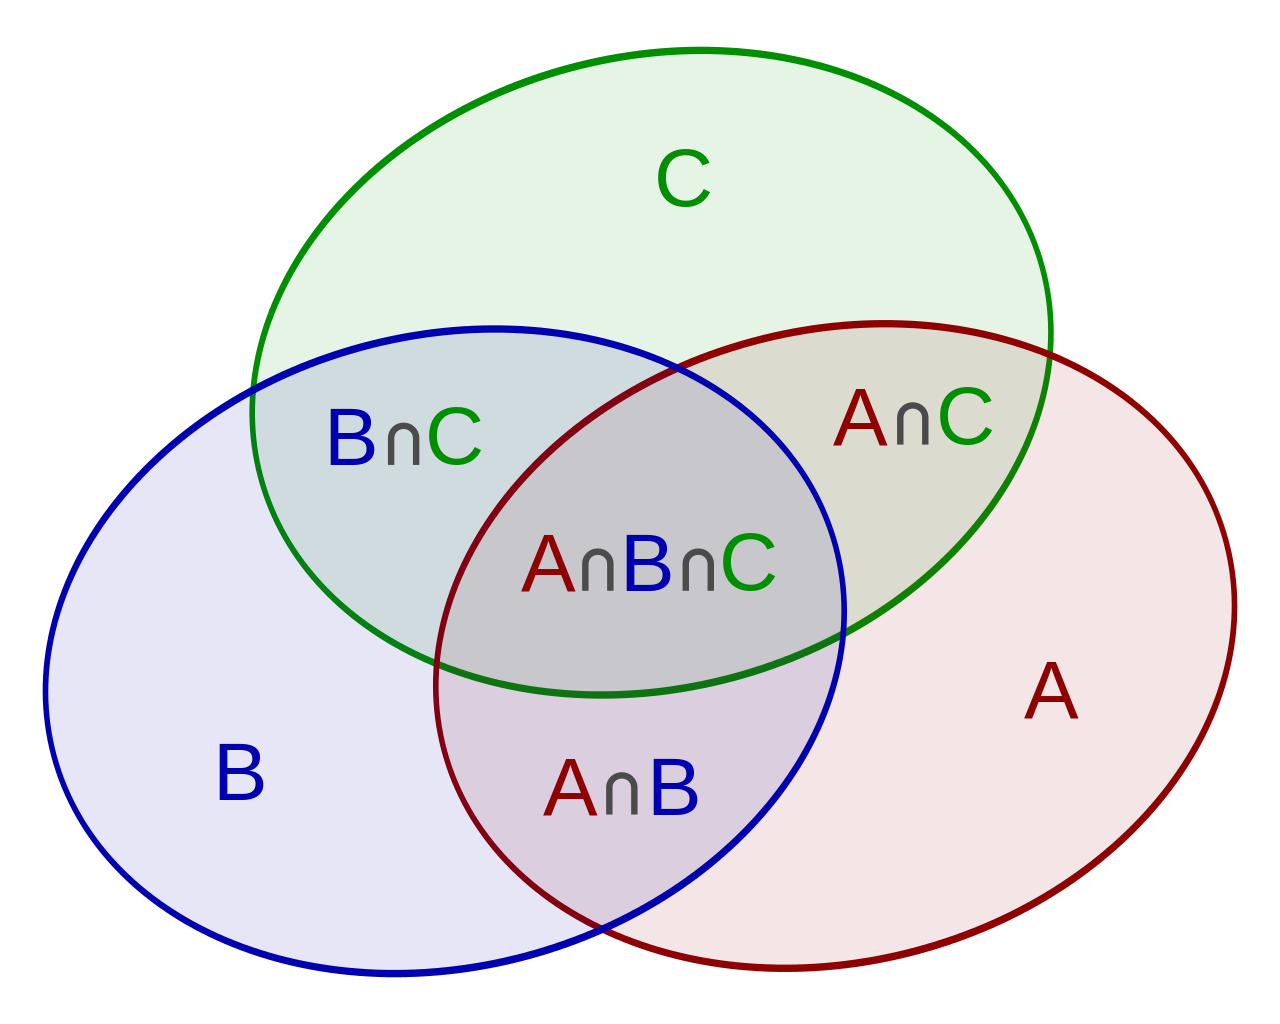
\includegraphics[scale=0.1]{nvi}
	\end{center}
\end{ex}

\begin{theorem}[NVI]
	\[|A_1 \cup \cdots \cup A_n| = \sum_{j = 1}^{n} (-1)^{j - 1} \sum_{1 \leqslant i_1 \leqslant \cdots \leqslant i_j \leqslant n}|A_{i_1} \cap A_{i_2} \cap \cdots \cap A_{i_j}|\]
\end{theorem}
\begin{defn}
	\[A_I := \displaystyle \bigcap_{i \in I} A_i \]
\end{defn}
\begin{ex}
	$A_{\{1,4,6,7\}} = A_1 \cap A_4 \cap A_6 \cap A_7$
\end{ex}
\begin{ex}
	$A_{\emptyset} = \cap_{i \in \emptyset} \ A_i = \{a; \ a \in A \ \land \ \forall i \in \emptyset\ a \in A_i \} = A$
\end{ex}
\begin{theorem}[Poenostavljen zapis NVI]
	\[|\bigcup_{i = 1}^{n} A_i| = \sum_{\emptyset \neq I \subseteq [n]} (-1)^{|I| - 1} |A_i|\]
\end{theorem}
\begin{theorem}[Druga oblika NVI]
	\[|\bigcap_{i = 1}^n A_i^c|  = \sum_{I \subseteq [n]} (-1)^{|I|} |A_I|\]
\end{theorem}
\begin{proof}
	Ozna"cimo $A_1, \ldots, A_n \subseteq A$ in se spomnimo, da $A_\emptyset = A$
	\[
		|\bigcap_{i = 1}^n A_i^c| =
		|(\bigcup_{i = 1}^n A_i)^c| =
		|A| - |\bigcup_{i = 1}^n A_i| =
		|A_{\emptyset}|\sum_{\emptyset \neq I \subseteq [n]} (-1)^{|I|} (A_I) =
		\sum_{I \subseteq [n]} (-1)^{|I|} |A_I|
	\]
\end{proof}


\begin{lemma}
\[k \geqslant 1 \implies \sum_{j = 0}^k (-1)^j \binom{k}{j} = 0\]
\end{lemma}

\begin{proof}
	V binomski izrek vstavimo $x = -1$
	\[(1 -1)^n = \sum_{j = 0}^k \binom{k}{j} x^j = 0\]
\end{proof}

\begin{rem}
	Lema pravi $\sum_{j \text{ sod}} \binom{k}{j} = \sum_{j\text{ lih}} \binom{k}{j}$ oziroma "stevilo sodih podmno"zic je vedno enako "stevilu lihih podmno"zic.
\end{rem}

To lahko poka"zemo tudi s slede"co bijekcijo
\[\varphi: \{\text{sode podmno"zice }[k]\} \rightarrow \{\text{lihe podmno"zice }[k]\} \]
\[\varphi (S) = \begin{cases}S \setminus \{k\}: \quad k \in S  \\ S \cup \{k\}: \quad k \notin S \end{cases}\]

\begin{proof}(NVI)
	\label{TODO: tega ne bom gledu}
	\[a \in \bigcup_{i = 1}^{n} A_i \text{, a vsebovana v natanko k mno"zicah}\]
	Dokazati "zelimo, da je doprinos $a$-ju k vsoti na desni enak $1$.
	\[k - \binom{k}{2} + \binom{k}{3} - ... + (-1)^{k-1} \binom{k}{k} = \sum_{j = 1}^{k} (-1)^{j - 1} \binom{k}{j} = - (\sum_{j = 0}^{k} (-1)^j \binom{k}{j} - 1) = 1\]
	$k$ \ldots doprinos v prvi vrstici\\
	$\binom{k}{2}$ \ldots doprinos v drugi vrstici\\
	$\displaystyle \sum_{j = 0}^{k} (-1)^j \binom{k}{j}$ = 0 (po lemi)
\end{proof}

\subsection{Eulerjeva funkcija $\phi$} % $\varphi$
\begin{defn}[Eulerjeva funkcija]
	\[\phi (n) = |\{i \in [n] : \gcd(i, n) = 1\}|\]
\end{defn}

\begin{claim}
	\[\sum_{a | n} \phi (a) = n\]
	(= "stevilo "stevil med $1$ in $n$, ki so tuje $n$)
\end{claim}

\begin{proof}
	Zapi"simo $\frac{1}{n}$, $\frac{2}{n}$, $\frac{3}{n}$, \ldots, $\frac{n}{n}$ in jih pokraj"sajmo.

	\[
	\begin{tabular}{c c c c c c c c c c c c}

	$\frac{1}{12}$ & $\frac{2}{12}$ & $\frac{3}{12}$ & $\frac{4}{12}$ & $\frac{5}{12}$ & $\frac{6}{12}$ & $\frac{7}{12}$ & $\frac{8}{12}$ & $\frac{9}{12}$ & $\frac{10}{12}$ & $\frac{11}{12}$ & $\frac{12}{12}$\\
	\\
	$\frac{1}{12}$ & $\frac{1}{6}$ & $\frac{1}{4}$ & $\frac{1}{3}$ & $\frac{5}{12}$ & $\frac{1}{2}$ & $\frac{7}{12}$ & $\frac{2}{3}$ & $\frac{3}{4}$ & $\frac{5}{6}$ & $\frac{11}{12}$ & $\frac{1}{1}$

	\end{tabular}
	\]

	Ulomkov je $n$, imenovalci so delitelji "stevila $n$, "stevci so "stevila, ki so manj"sa od $a$ in tuja z $a$.
	\[\sum_{a | n} \phi (a) = n\]
\end{proof}

\begin{theorem}[Formula za $\phi$]
	\[\phi (n) = n \cdot \prod_{p | n} (1 - \frac{1}{p})\]
\end{theorem}
\begin{proof}
	\[A = [n], \quad n = p_1^{\alpha_1} \cdots p_k^{\alpha_k} \quad \alpha_i > 0\]
	\[A_i = \{j \in [n] : p_i | j\} \]
	\[|A_i| = \frac{n}{p_i}\]
	\[|A_i \cap A_j| = \frac{n}{p_i p_j}\]
	\[|A_I| = \frac{n}{\displaystyle \prod_{i \subseteq I} p_i}\]

	\[\phi (n) = \sum_{I \subseteq [k]} (-1)^{|I|} \frac{n}{\displaystyle \prod_{i \in I} p_i}\]

		$k = 2$ \label{TODO: k=2? kasn k? od kje? kaj to pomen}

	\[n\cdot(1 - \frac{1}{p_1} - \frac{1}{p_2} + \frac{1}{p_1 p_2}) = n\cdot(1 - \frac{1}{p_1})\cdot(1 - \frac{1}{p_2})\]
	\[\phi (n) \stackrel{\text{distributivnost}}{=}  n\cdot(1 - \frac{1}{p_1})\cdot(1 - \frac{1}{p_2})\cdot \ldots \cdot(1 - \frac{1}{p_k})\]

	\[\phi (n) = n \cdot \prod_{p | n} (1 - \frac{1}{p})\]
\end{proof}
%26. 10. 2021

\subsection{Multinomski koeficienti}
Spomnimo se na binomske koeficiente
\[\binom{n}{k} \ = \ \frac{n!}{k! (n - k)!}\text{, } 0 \leqslant k \leqslant n\]

Imamo $a$ enic in $b$ ni"cel. Preme"samo jih lahko na
\[\binom{a + b}{a} = \binom{a + b}{b} = \frac{(a+b)!}{a!b!}\]
na"cinov. Kaj pa "ce imamo ve"c enakih elementov? "Stevila $1,1,1,2,2,3,3,3,3,3,4$ lahko preme"samo na.
\[\binom{a_1 + a_2 + ... + a_n}{a_1} \cdot \binom{a_2 + a_3 ... + a_n}{a_2} \cdot \binom{a_3 + a_4 + ... + a_n}{a_3} ...\]
na"cinov. V prvem binomu izberemo enke, v drugem dvojke, v tretjem trojke~\ldots. To razpi"semo kot
\[\frac{(a_1 + a_2 + ... + a_n)!}{a_1!(a_2 + a_3 + ... + a_n)!} \cdot \frac{(a_2 + a_3 + ... + a_n)!}{a_2!(a_3 + a_4 + ... + a_n)!} \cdot \frac{(a_3 + a_4 + ... + a_n)!}{a_1!(a_4 + a_5 + ... + a_n)!} ... \frac{(a_{n-1}+a_n)!}{a_{n-1}!a_n!} =\]
\[= \frac{(a_1 + a_2 + ... + a_n)!}{a_1!a_2!...a_n!} = \frac{(\displaystyle \sum_{i = 1}^n a_i)!}{\displaystyle \prod_{i = 1}^n a_i!} = \binom{a_1 + a_2 + ... + a_n}{a_1, a_2, ..., a_n}\]

Alternativno: dodamo indekse $1_1, 1_2, 1_3, 2_1, 2_2, 3_1, 3_2, 3_3, 3_4, 3_5, 4_1$. Preme"samo na
\[\frac{(a_1 + a_2 + ... + a_n)!}{a_1!a_2!...a_n!}\]
na"cinov; najprej smo preme"sali vse na $(a_1 + a_2 + ... + a_n)!$ na"cinov, potem pa z $a_i!$ izbrisali indekse)\\

\begin{rem}
	\[\binom{a+b}{a, b} = \frac{(a+b)!}{a!b!} = \binom{a+b}{a} = \binom{a+b}{b}\]
\end{rem}

\begin{theorem}[Multinomski izrek]
	\[(x_1 + x_2 + \cdots + x_n)^m = \sum_{(a_1, \ldots, a_n)_{\text{ "sibka kompozicija }m}} \binom{m}{a_1, \cdots, a_n} x_1^{a_1}\cdots x_n^{a_n}\]
\end{theorem}

\begin{proof}
	\[(x_1 + x_2 + \cdots + x_n)\cdot(x_1 + x_2 + \cdots + x_n)\cdot\ldots\cdot(x_1 + x_2 + \cdots + x_n)\]
	Iz vsakega oklepaja izberemo $x_i$, kar skupaj pride $x_1^{a_1} x_2^{a_2}...x_n^{a_n}$, pri "cemer je $\displaystyle \sum_{i = 1}^n a_i$ = m, $a_i \geqslant 0$. Koeficient je o"citno $\binom{a_1 + a_2 + ... + a_n}{a_1, a_2, ..., a_n}$.
\end{proof}

\begin{ex}
	$x_1 = x_2 = ... = x_n$
	\[n^m = \sum_{(a_1, ..., a_n)_{\text{"sibka kompozicija m}}} \binom{m}{a_1, ..., a_n}\]
\end{ex}


\subsection{Na"crti in t-na"crti}
Podjetje proizvaja ve"c razli"cic izdelka, "zeli jih testirati pri potro"snikih. Vsak potro"snik mora testirati enako "stevilo razli"cic, vsako razli"cico mora testirati enako "stevilo potro"snikov.

\[1234, 1247, 1357, 2468, 3568, 5678\]
$8$ razli"cic, $6$ potro"snikov, vsak potro"snik testira $4$, vsako razli"cico testirajo $3$ potro"sniki.

\begin{defn}[Na"crt]
	$B = \{B_1, \ldots, B_b\}$ je nar"ct s parametri $(v, k, \lambda)$, kadar velja
	\begin{itemize}
		\item $B_1, \ldots, B_b \subseteq [v]$
		\item $|B_1| = \ldots = |B_b| = k$
		\item vsak $i \in [v]$ se pojavi v natanko $\lambda$ mno"zicah oz. ``blokih''.
	\end{itemize}
\end{defn}

\begin{ex}
	Na"crt s parametri $(8, 4, 3)$.\\
	Nari"semo tabelo
	\begin{tabular}{c|c c c}
		& $B_1$ & ... & $B_b$ \\
		\hline
		1 \\
		...\\
		v
	\end{tabular}\\
	Kljukico damo tam, kjer je $i \in B_j$. V vsakem stolpcu tako dobimo $k$ kljukic, skupaj $k\cdot b$, v vsaki vrstici dobimo $\lambda$ kljukic, skupaj $\lambda \cdot v$. Iz tega sledi, da $k \cdot b = \lambda \cdot v$, oziroma $b = \frac{\lambda v}{k}$

	Velja "se b $\leqslant$ $\binom{v}{k}$
	\[\frac{\lambda v}{k} \leqslant \frac{v!}{k! (v-k)!}\]
	Pokraj"samo $\frac{v}{k}$ na obeh straneh neena"cbe in dobimo
	\[\lambda \leqslant \frac{(v - 1)!}{(k - 1)! (v - k)!} = \binom{v-1}{k-1}\]
\end{ex}

\begin{theorem}\mbox{}\\
	Na"crt s parametri $(v, k, \lambda)$ obstaja natanko tedaj, ko velja $k | v\cdot \lambda$ in $\lambda \leqslant \binom{v - 1}{k - 1}$
\end{theorem}

\begin{proof}\mbox{}\\
	($\Rightarrow$) "Ze dokazano.\\
	($\Leftarrow$) Izberemo $\frac{\lambda v}{k}$ $k$-elementnih podmno"zic mno"zice $[v]$. To lahko naredimo, ker je $\frac{\lambda v}{k} \leqslant \binom{v - 1}{k - 1}\cdot \frac{v}{k} = \binom{v}{k}$.\\

	\[v = 8, \ k = 4, \ \lambda = 3\]
	\[\frac{\lambda v}{k} = 6  \Rightarrow 1234, 1356, 1567, 1568, 2356, 3457\]
	To ni nujno na"crt.
	\[\lambda_i \text{ \ldots v koliko blokih je vsebovan }i\]
	\[\lambda_1 = 4,\ \lambda_2 = 2,\ \lambda_3 = 4,\ \lambda_4 = 2,\ \lambda_5 = 5,\ \lambda_6 = 4,\ \lambda_7 = 2,\ \lambda_8 = 1\]
	Naredimo isto tabelo kot prej in ugotovimo, da je $\lambda = \frac{\sum_{i = 1}^v \lambda_i}{v}$.\\
	"Ce to ni na"crt, zagotovo obstajata $i$, $j$, da je $\lambda_i$ > $\lambda$ > $\lambda_j$.\\

	Bloki so 4 tipov:
	\begin{itemize}
	    \item[(I)] vsebujejo $i$ in $j$
	    \item[(II)] vsebujejo $i$, ne pa $j$
	    \item[(III)] vsebujejo $j$, ne pa $i$
	    \item[(IV)] ne vsebujejo ne $i$ ne $j$\\
	\end{itemize}

	Bloki tipa (I) in (IV) vsebujejo enako $i$-jev in $j$-jev.
	\begin{itemize}
	    \item[] $\lambda_i$ = blokov tipa (I) + (II)
	    \item[] $\lambda_j$ = blokov tipa (I) + (III)
	\end{itemize}
	Sledi, da je ve"c blokov tipa (II) kot (III). Iz tega sledi, da obstaja blok tipa (II), tako da po zamenjavi $i$ z $n$ ne dobimo "ze obstoje"cega bloka.\\
	\[ 1234, 1356, \textcolor{red}{2}567, 1568, 2356, 3457 \]
	V splo"snem: $\lambda_i\!\mathrel{--},\ \lambda_j\!\mathrel{++}$\\
	Postopek ponovimo, dokler ni $\lambda_1 = \lambda_2 = ... = \lambda_6$
	\[1234, 1\textcolor{red}{4}56, 2567, 1568, 2356, 3457\]
	\[1234, 145\textcolor{red}{7}, 2567, 1568, 2356, 3457\]
	\[1234, 1457, 267\textcolor{red}{8}, 1568, 2356, 3457\]
	\[1234, 147\textcolor{red}{8}, 2678, 1568, 2356, 3457\]
	kar je na"crt.\\
	Na vsakem koraku se zmanj"sa $\displaystyle \sum_{i = 1}^v (\lambda_i - \lambda)$ za $2$, po kon"cno korakih je to = $0$ in dobimo na"crt.
\end{proof}

\begin{defn}[$t$-na"crt]
	$B = \{B_1, \ldots, B_b\}$ je $t$-nar"ct s parametri $(v, k \lambda_t)$, kadar velja
	\begin{itemize}
		\item $B_1, \ldots, B_b \subseteq [v]$
		\item $|B_1| = \cdots = |B_b| = k$
		\item vsaka $t$-elementna podmno"zica $[v]$ je vsebovana v to"cno $\lambda_t$ blokih.
	\end{itemize}
\end{defn}
\begin{rem}
	$1$-na"crt = na"crt
\end{rem}
\begin{ex}
	$124, 137, 156, 235, 267, 346, 457$ je $2$-na"crt $(7, 3, 1)$
\end{ex}
\begin{rem}
	Tudi na"crt s parametri $(7, 3, 3)$ NI $3$-na"crt!!
\end{rem}

\label{TODO: add explanation, kaj je point?}
\begin{figure}[h!]
	\centering
	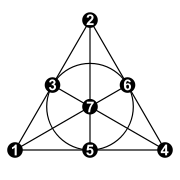
\includegraphics[scale=0.5]{fano_plane}
	\caption{Fanova ravnina}
\end{figure}

\begin{theorem}
	"Ce je $B$ $t$-na"crt s parametri $(v, k, \lambda_t)$, je tudi $(t-1)$-na"crt s parametri $(v, k, \lambda_{t-1})$. Velja formula
	\[\lambda_{t-1} = \lambda_t \cdot \frac{v - t + 1}{k - t + 1}\]
\end{theorem}

\begin{proof}
	$S \subseteq [v]$, $|S| = t - 1$. $S$ je vsebovana v $\lambda_s$ blokih.
	Nari"semo tabelo
	\begin{center}
		\begin{tabular}{c|c c c c c}
		     & $B_1$ & $\cdots$ & j & $\cdots$ & $B_b$ \\
		\hline
		     1 \\
		     \vdots \\
		     i & & & \checkmark\\
		     \vdots \\
		     v
		\end{tabular}
	\end{center}
	$i \notin S$, $S \cup \{i\} \subseteq B_j$. Skupno je po stolpcih:
	\begin{itemize}
	    \item $S\setminus B_j$: $0$ kljukic
	    \item $S \subseteq B_j$: $k-t+1$ kljukic
	    \item[] skupaj: $\lambda_s (k-t+1)$
	\end{itemize}
	in po vrsticah:
	\begin{itemize}
	    \item $i\in S$: $0$ kljukic
	    \item $i\notin S$: $\lambda_t$ kljukic
	    \item[] skupaj: $\lambda_t (v-t+1)$
	\end{itemize}

	\[\implies \lambda_s = \frac{(v - t + 1)\lambda_t}{k-t+1}\]
\end{proof}



\section{Permutacije, razdelitve, raz"clenitve}
\subsection{Stirlingova "stevila prve vrste}
$\pi \in S_n$ lahko zapi"semo kot produkt disjunktnih ciklov
\[\cycle{1, 4, 6, 3, 5, 8, 2, 7} = \cycle{1}\cycle{2, 4, 3, 6, 8, 7}\cycle{5}\]

\begin{defn}[Stirlingovo "stevilo prve vrste]
	Je "stevilo permutacij v $S_n$, ki imajo natanko $k$ ciklov (negibne to"cke "stejemo kot cikle dol"zine $1$). Ozna"cimo $c(n, k)$
\end{defn}
Za $c(n, k)$ ni ``lepe'' formule. Vemo pa naslednje lastnosti
\begin{itemize}
	\item $c(n, n) = 1$
	\item $c (n, n-1) = \binom{n}{2}$ (transpozicija)
	\item $c(n, 0) = 0$ ("ce $n > 0$, oziroma $1$, "ce je $n = 0$)
	\item $c(n, 1) = (n-1)!$
	\item $c(n, k) = 0$ za $k > n$ ali $k < 0$
	\item $\sum_k c(n, k) = n!$
\end{itemize}

\begin{claim}[Rekurzivna zveza]
	\[c(n, k) = c(n-1, k-1) + c(n-1, k)\cdot(n-1)\]
\end{claim}

\begin{proof}
	Permutacije v $S_n$ s $k$ cikli:
	\begin{itemize}
	    \item $n$ je negibna to"cka: $c(n-1, k-1)$
	    \item $n$ ni negibna to"cka: $c(n-1, k)  \cdot (n-1)$ ((izbri"sem $n$, dobim permutacijo v $S_{n-1}$ s $k$ cikli) $\cdot$ (vsako dobimo $(n-1)$-krat))
	\end{itemize}
\end{proof}


% 2.11.2021 by Toma"z
%\begin{Toma"z}
Tabela Stirlingovih "stevil 1. vrste:
\begin{center}
	\begin{tabular}{l|llllll}
	    $n \backslash k$ & 0 & 1  & 2  & 3  & 4  & 5 \\
	    \hline
	    0 & 1 & 0  & 0  & 0  & 0  & 0 \\
	    1 & 0 & 1  & 0  & 0  & 0  & 0 \\
	    2 & 0 & 1  & 1  & 0  & 0  & 0 \\
	    3 & 0 & 2  & 3  & 1  & 0  & 0 \\
	    4 & 0 & 6  & 11 & 6  & 1  & 0 \\
	    5 & 0 & 24 & 50 & 36 & 10 & 1
	\end{tabular}
\end{center}
Konstruiramo podobno kot Pascalov trikotnik za binomske koeficiente (\ref{pascalov_trikotnik}), samo da uporabimo drugo rekurzivno formulo; najprej damo diagonalne elemente na $1$, naddiagonalne na $0$, $1$. stoplec na 0 (razen prvega elementa, ki je "ze $1$), za ostale pa uporabimo rekurzivno forumlo (se"stejemo element levo zgoraj in $(n-1)$ krat zgornji). \label{konstrukcija_tabele}

\begin{claim}[Rekurzivna zveza]\label{rekurzivna_cnk_narascajoce}
    \[\sum_k c(n,k)x^k = x^{\overline{n}}\]
\end{claim}

\begin{proof}
    Indukcija po $n$:\\
    Baza indukcije: $n = 0: (1x^0 = x^0)$. OK.\\
    Indukcijski korak: $n - 1 \implies n$:\\
    \[x^{\overline{n}} = x^{\overline{n-1}}(x+n-1) = \sum_k c(n-1,k)x^k (x+n-1) =\]
    \[= \sum_k c(n-1,k)x^{k+1} + \sum_k c(n-1,k)x^k (n-1) = \]
    \[\sum_k c(n-1,k-1)x^{k} + \sum_k c(n-1,k)x^k (n-1) =\]
    \[= \sum_k c(n,k)x^k\]
\end{proof}

\begin{proof}
	Alternativno, lahko gremo tudi v obratni smeri.
	\[x \leftrightarrow -x\] \label{TODO: I see x <-> -x, I skip.}
	\[\sum_k c(n,k) (-1)^k x^k = (-x)^{\overline{n}}\]
	\[\sum_k (-1)^{n-k} c(n,k) x^k = x^{\underline{n}}\]
	$s(n,k) := (-1)^{n-k} c(n,k)$ predzna"ceno stirlingovo "stevilo prve vrste
	\[\sum_k s(n,k) x^k = x^{\underline{n}}\]
\end{proof}

\begin{proof}
	"Se eno alternativo tega dokaza bomo naredili pri P\'olyjevi teoriji (\ref{polyeva_dokaz_rekurzivne_cnk}).
\end{proof}

\subsection{Stirlingova "stevila druge vrste}
\begin{defn}[Razdelitev mno"zice]
    Razdelitev, razbitje ali particija je $\{B_1 \cdots B_n\}$, pri "cemer
    \begin{itemize}
        \item $B_i \neq \emptyset \quad i = 1 \ldots k$
        \item $B_i \cap B_j = 0 \text{ za } i \neq j$
        \item $\cup_{i=0}^k B_i = A$
        \item $B_1 \dots B_n \text{ so bloki razdelitve}$
    \end{itemize}
\end{defn}

\begin{ex}
	\[A = [8]: \{ \{1, 4, 5\} \{2\} \{3, 6, 7, 8\}\} \equiv 145-2-3678 \equiv 2-415-8763\]
\end{ex}
\begin{rem}
	"Ce je $R$ je ekvivalen"cna relacija nad $A$ (refleksivna, simetri"cna, tranzitivna), je mno"zica ekvivalen"cnih razredov $R$ ravno razdelitev mno"zice $A$.
\end{rem}

\begin{defn}[Stirlingovo "stevilo druge vrste]
    $S(n,k)$ je "stevilo razdelitev $[n]$ z natanko $k$ bloki.
\end{defn}
\begin{defn}[Bellovo "stevilo]
	$B(n)$ je "stevilo razdelitev $[n]$. Velja
	\[B(n) = \sum_k S(n,k)\]
\end{defn}

\begin{rem}
	$B(n) \neq B_n$. $B_n =$ Bernoulijevo "stevilo
\end{rem}

Preproste formule za $S(n,k)$ in $B(n)$ nimamo, poznamo pa naslednje identitete:
\begin{itemize}
	\item $S(n,n) = 1$
	\item $S(n,n-1) = \binom{n}{2}$
	\item $S(n,1) = 1 - \delta_{n0}$
	\item $S(n,0) = \delta_{n0}$
	\item $S(n,k) = 0$ za $k < 0$ ali $k > n$
	\item $S(n,k) \leq c(n,k)$
\end{itemize}

\begin{claim}[Rekurzivna formula za $S(n)$]
    \[S(n, k) = S(n-1, k-1) + k \cdot S(n-1, k)\]
\end{claim}

\begin{proof}
    Razdelitve $[n]$ s $k$ bloki:
    \begin{itemize}
        \item $n$ je (samostojen) blok: $S(n-1, k-1)$
        \item $n$ je v bloku velikosti $\geq 1$: $k \cdot S(n-1, k)$ ($n$ lahko vstavimo v katerega koli izmed $k$ blokov: $n$ vstavimo nazaj na $k$ na"cinov)
    \end{itemize}
\end{proof}

\begin{center}
	\begin{tabular}{l|llllll|l}
	    $n \backslash k$ & 0 & 1  & 2  & 3  & 4  & 5 & $B(n)$ \\
	    \hline
	    0 & 1 & 0  & 0  & 0  & 0  & 0 & 1 \\
	    1 & 0 & 1  & 0  & 0  & 0  & 0 & 1 \\
	    2 & 0 & 1  & 1  & 0  & 0  & 0 & 2 \\
	    3 & 0 & 1  & 3  & 1  & 0  & 0 & 5 \\
	    4 & 0 & 1  & 7  & 6  & 1  & 0 & 15 \\
	    5 & 0 & 1  & 15 & 25 & 10 & 1 & 52
	\end{tabular}
\end{center}

\begin{rem}
	Za konstrukcijo glej Stirlingova "stevila prve vrste.
\end{rem}

\begin{claim}[Pomen $S(n)$]
    $S(n,k)$ je "stevilo ekvivalen"cnih relacij na $[n]$ s k ekvivalen"cnimi razredi. $B(n)$ je "stevilo ekvivalen"cnih relacij na $[n]$
\end{claim}

\begin{claim}
    "Stevilo surjekcij $[n] \rightarrow [k]$ je $k! \cdot S(n,k)$
\end{claim}

\begin{proof}
    Naj bo $f: [n] \rightarrow [k]$ surjekcija.
    Mno"zica $\{f^{-1}(1), f^{-1}(2) \cdots f^{-1}(k)\}$, kjer $f^{-1}(i)$ predstavlja mno"zico praslik $i$-ja $(=\{j: f(j) = i\}$) je razdelitev $[n]$ s $k$ bloki. Vsaka razdelitev $[n]$ s $k$ bloki nam da $k!$ surjekcij
    (bloke linearno uredimo).
    \\
    Ekvivalentno: urejena razdelitev $\equiv$ surjekcija.
\end{proof}

\begin{conseq}
	\[S(n,k) = \frac{1}{k!} \sum_{j=0}^k (-1)^{k-j} \binom{k}{j}j^n = \sum_{j=0}^k \frac{(-1)^{k-j} j^n}{j! (k-j)!}\]
\end{conseq}

\begin{claim}[Rekurzivna formula za $S(n)$]
    \[\sum_k S(n,k)x^{\underline{k}} = x^n\]
\end{claim}

\begin{proof}(1. na"cin)
	Z indukcijo (na vajah, DN?)
\end{proof}
\begin{proof}(2. na"cin)
    Naj bo $x \in \N$.
    $x^n$ je "stevilo preslikav iz $[n]$ v $[k]$.
    Vsaka preslikava je surjekcija na svojo sliko (zalogo vrednosti).
    \[x^n = \sum_T \big(|T|! \cdot S(n,|T|)\big) = \sum_k \big(k! \cdot S(n,k) \cdot \binom{x}{k}\big)\]
    kjer je $T$ slika preslikave, $\binom{x}{k} = \frac{x^{\underline{k}}}{k!}$ pa predstavlja "stevilo $k$-elementnih podmno"zic od $[x]$.
\end{proof}

\label{TODO: surprise analiza? kaj so te polinomi kle?}
Dva polinoma stopnje $\leq n$, ki se ujemata v $n+1$ to"ckah, sta enaka (razlika je polonom stopnje $\leq n$ z $n+1$ ni"clami, torej je ekvivalentna 0)

$\sum_k S(n,k)x^{\underline{k}}$ in $x^n$ sta polinoma stopnje $n$, ujemata se v neskon"cno to"ckah (ker gremo v vsoti po vseh $x \in \Z(\N)$), torej sta enaka.
\\
Velja tudi: \[\sum_k (-1)^{n-k} S(n,k) x^{\overline{k}} = x^n\]

\begin{claim}[Rekurzivna formula za $B(n)$]
    \[B(n+1) = \sum_{k=0}^n \binom{n}{k} B(k)\]
\end{claim}

\begin{proof}
    Izberemo razdelitev $[n+1]$ ($k$ je "stevilo elementov), ki so v istem bloku kot $n+1$
    \[B(n+1) = \sum_{k=0}^n \binom{n}{k}B(n-k)\]
    $\binom{n}{k}$: izbira elementov, ki so v istem bloku (skupaj z $n+1$). \\
    $B(n-k)$: izberemo razdelitev na preostalik $n-k$ elementih (ta izbira je neodvisna in takih je $B(n-k)$).
    \[k \rightarrow n-k: \quad B(n+1) = \sum_{k=0}^n \binom{n}{k}B(k)\]
\end{proof}
%%

\subsection{Lahova "stevila}
\begin{defn}[Lahovo "stevilo]
	$L(n,k)$ je "stevilo razdelitev $[n]$ na k linearno urejenih blokov.
\end{defn}
\begin{rem}
	Spomnimo se: $S(n,k)$ je "stevilo razdelitev $[n]$ na $k$ blokov, $c(n,k)$ pa "stevilo razdelitev $[n]$ na $k$ cikli"cno urejenih blokov.
\end{rem}


\begin{itemize}
	\item $L(n,n) = 1$
	\item $L(n,n-1) = 2$
	\item $\binom{n}{2} = n(n-1)$
	\item $L(n,0) = \delta_{n0}$
	\item $L(n,1) = n!$
	\item $L(n,k) = 0$ za $k < 0$ ali $k > n$
	\item $S(n,k) \leq c(n,k) \leq L(n,k)$
\end{itemize}

\begin{claim}[Rekurzivna formula za $L(n, k)$]
    \[L(n,k) = \frac{n!}{k!} \binom{n-1}{k-1}\]
\end{claim}
\begin{proof}
    Pre"stejemo urejene razdelitve $[n]$ s $k$ linearno urejenimi bloki
    \[ k! \cdot L(n,k) = n! \cdot \binom{n-1}{k-1} \]
    $k!$ - uredimo bloke, $n!$ - premutacija, $\binom{n-1}{k-1}$ - kompozicija
\end{proof}

\begin{claim}
    \[L(n,k) = L(n-1, k-1) + (n-1+k) L(n-1, k)\]
\end{claim}
\begin{proof}
    Ekvivalentno kot ostale rekurzije, samo ``podrobnost'' $(n-1+k)$: $n$ vstavimo za obstoje"cim "stevilom $(n-1)$ ali pa na za"cetek bloka ($k$)
\end{proof}

Primerjajmo rekurzije:
\begin{itemize}
    \item $\binom{n}{k} = \binom{n-1}{k-1} + \binom{n-1}{k}$
    \item $c(n,k) = c(n-1, k-1) + (n-1) \cdot c(n-1, k)$
    \item $S(n,k) = S(n-1, k-1) + k\cdot S(n-1, k)$
    \item $L(n,k) = L(n-1, k-1) + (n-1+k)\cdot L(n-1, k)$
\end{itemize}

\begin{claim}[Rekurzivna formula za $L(n, k)$]
    \[ \sum_k L(n,k)x^{\underline{k}} = x^{\overline{n}}\]
\end{claim}
\begin{proof}
    Dokaz bomo prepustili bralcu za vajo
\end{proof}

Primerjajmo:
\begin{itemize}
    \item $\sum_k \binom{n}{k}x^k = (1+x)^n$
    \item $\sum_k C(n,k)x^k = x^{\overline{n}} \quad \sum_k (-1)^{n-k}C(n,k)x^k = x^{\underline{n}}$
    \item $\sum_k S(n,k)x^{\underline{k}} = x^n \quad \sum_k (-1)^{n-k}S(n,k)x^{\overline{k}}x^n$
    \item $\sum_k L(n,k)x^{\underline{k}} = x^{\overline{{n}}} \quad \sum_k (-1)^{n-k}L(n,k)x^{\overline{{n}}}x^{\underline{k}}$
\end{itemize}

%\end{Toma"z}
% 9. 11. 2021

\subsection{Raz"clenitve naravnih "stevil in Eulerjev petkotni"ski izrek}
\begin{defn}[Raz"clenitev naravnega "stevila]
	Raz"clenitev ali particija $n \in \N$ je $l$-terica
	\[\lambda = (\lambda_1, \lambda_2, ..., \lambda_l)\]
	\[\lambda_1 \geqslant \lambda_2 \geqslant ... \geqslant \lambda_l > 0\]
	\[\lambda_1 + \lambda_2 + \cdots + \lambda_l = n\]
	$\lambda_i$ so "cleni raz"clenitve, $n$ je velikost raz"clenitve, $l$ je dol"zina raz"clenitve.
\end{defn}

\begin{ex}
	$(5, 4, 4, 2, 1, 1)$ je raz"clenitev "stevila $17$ s $6$ "cleni.
\end{ex}
\begin{rem}
	Ozna"cimo tudi $5 + 4 + 4 + 2 + 1 + 1$ ali $5\ 4\ 4\ 2\ 1\ 1$.
\end{rem}

Raz"cletnive lahko prika"zemo grafi"cno s pomo"cjo Ferresovih diagramov.
\begin{ex}
	Diagram za $\lambda = (5, 4, 3, 2, 1, 1)$
	\[
		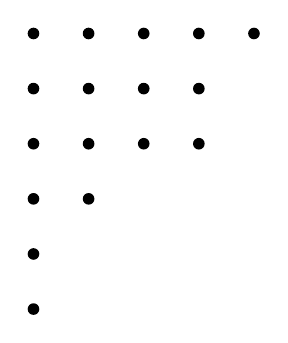
\begin{tikzpicture}[scale=0.7]
		 \fill foreach \Z [count=\Y] in {5,4,4,2,1,1}
		  {foreach \X in {1,...,\Z}
		  {(\X,-\Y) circle[radius=3pt]}};

		\end{tikzpicture}
	\]
\end{ex}

\begin{defn}[Raz"clenitve]\mbox{}
	\begin{itemize}
		\item S $p(n)$ ozna"cimo "stevilo vseh raz"clenitev $n$.
		\item S $p_k(n)$ ozna"cimo "stevilo raz"clenitev $n$ s $k$ "cleni.
		\item S $\overline{p_k}(n)$ ozna"cimo "stevilo raz"clenitev $n$ z $\leqslant k$ "cleni.
	\end{itemize}
\end{defn}
\begin{rem}
	Ni lepe formule za $p(n)$, $p_k(n)$ ali $\overline{p_k}(n)$.
\end{rem}

\begin{ex}\mbox{}\\
	$n = 0: (), p(0) = 1, p_0(0) = 1$\\
	$n = 1: 1$\\
	$n = 2: 2, 1 1$\\
	$n = 3: 3, 2 1, 1 1 1$\\
	$n = 4: 4, 3 1, 2 2, 2 1 1, 1 1 1 1$\\
	$n = 5: 5, 4 1, 3 2, 3 1 1, 2 2 1, 2 1 1 1, 1 1 1 1 1$\\
	$p(n) : 1, 1, 2, 3, 5, 7, 11, 15, \ldots$\\
	$p_2(5) = 2$\\
	$\overline{p_3}(5) = 5$
\end{ex}

\begin{defn} [Konjugirana raz"clenitev $\lambda '$]
	Dobimo s transpozicijo Ferresovega diagrama (stolpce napi"semo kot vrstice).
\end{defn}
Veljajo naslednje lastnosti:
\begin{itemize}
	\item $\lambda_i ' = |\{i: \lambda_j \geqslant i\}| = \max\{j: \lambda_j \geqslant i\}$
	\item $\lambda '' = \lambda$
	\item $\lambda_1 ' = l(\lambda)$
	\item $l(\lambda ') = \lambda_1$
\end{itemize}
\begin{ex}
	$5 \ 4 \ 4 \ 2 \ 1 \ 1 ' = 6 \ 4 \ 3 \ 3 \ 1$
\end{ex}

\begin{claim}[Lastnosti $p_k(n)$]\mbox{}
	\begin{enumerate}
	    \item $p_k(n)$ = $\overline{p_{k - 1}} (n - k)$
	    \item $p_k(n)$ = $p_{k - 1} (n - 1)$ + $p_k (n - k)$
	    \item $\overline{p_{k}}(n)$ = $\overline{p_{k - 1}}(n) + p_k (n)$ = $\overline{p_{k - 1}}(n) + \overline{p_k} (n - k)$
	\end{enumerate}
\end{claim}

\begin{proof}
	Precej trivialno;
    \begin{enumerate}
        \item Izbri"semo / dodamo prvi stolpec / stolpec dol"zine k
        \item Imamo raz"clenitev $n$ s $k$ "cleni: $\lambda_l = 1$ ($p_{k - 1}(n - 1)$) in $\lambda_l \geqslant 2$ ($p_k(n - k)$)
        \item O"citno
    \end{enumerate}
\end{proof}

\begin{rem}
	Do zdaj obravnavane rekurzivne formule):\\
	\begin{itemize}
	    \item $\binom{n}{k} = \binom{n - 1}{k - 1} + \binom{n - 1}{k}$
	    \item $c(n, k) = c(n - 1, k - 1) + (n - 1)\cdot c(n - 1, k)$
	    \item $S(n, k) = S(n - 1, k - 1) + k\cdot S(n - 1, k)$
	    \item $L(n, k) = L(n - 1, k - 1) + (n + k - 1)\cdot L(n - 1, k)$
	    \item $p_k(n) = p_{k - 1}(n - 1) + p_k (n - k)$
	    \item $\overline{p_k}(n) = \overline{p_{k - 1}}(n) + \overline{p_k}(n - k)$
	\end{itemize}
\end{rem}

Tabela za $p_k(n)$:
\begin{tabular}{c|c c c c c c c|c}
    $n \backslash k$ & 0 & 1 & 2 & 3 & 4 & 5 & 6 & $\sum_k p_k(n) = p(n)$\\
    \hline
    0 & 1 & 0 & 0 & 0 & 0 & 0 & 0 & 1 \\
    1 & 0 & 1 & 0 & 0 & 0 & 0 & 0 & 1 \\
    2 & 0 & 1 & 1 & 0 & 0 & 0 & 0 & 2 \\
    3 & 0 & 1 & 1 & 1 & 0 & 0 & 0 & 3 \\
    4 & 0 & 1 & 2 & 1 & 1 & 0 & 0 & 5 \\
    5 & 0 & 1 & 2 & 3 & 1 & 1 & 0 & 7 \\
    6 & 0 & 1 & 3 & 3 & 2 & 1 & 1 & 11 \\
\end{tabular}\\
Za postopek izpolnitve tabele glej Stirlingova "stevila 1. vrste (\ref{konstrukcija_tabele}). Uporabi formulo $p_k(n) = p_{k - 1}(n - 1) + p_k(n - k)$.

\label{TODO: why is this commented out}
%\begin{itemize}
%    \item $p_n$(n) = 1 (diagonalni elementi so enice)
%    \item $p_k$(n) = 0, k > n (elementi nad diagonalo so 0)
%    \item $p_1$(n) = n, n $\geqslant$ 1
%    \item $p_2$(n) = $\lfloor \frac{n}{2} \rfloor$
%    \item $\overline{p_n}$(n) = p(n)
%\end{itemize}

Kaj pa rekurzija za $p(n)$?
\[A = \{\text{raz"clenitve }n\} = \bigcup_{i = 1}^n A_i\]
\[A_i = \{\text{raz"clenitve }n\text{, ki vsebujejo }i\text{ kot "clen}\}\]
\[|A_i| = p(n - i)\]
\[|A_i \bigcap_{i \neq j} A_j| = p(n - i - j)\]
\[|A_I| = p(n - \sum_{i \in I} i)\]
\begin{align}
	|\bigcup_{i = 1}^n A_i| = & |A_1| + ... + |A_n|\nonumber\\
    			& - |A_1 \cap A_2| - |A_1 \cap A_3| ...\nonumber\\
                & + |A_1 \cap A_2 \cap A_3| ...\nonumber\\
                & - ...\nonumber\\
                & + ...\nonumber
\end{align}
\label{TODO: tukej pogresam malo texta}
\begin{align}
	p(n) = & p(n - 1) + p(n - 2) + \cancel{p(n - 3)} + \cancel{p(n - 4)} + \cancel{p(n - 5)} + ...\nonumber\\
    	& - \cancel{p(n - 1 - 2)} - \cancel{p(n - 1 - 3)} - \cancel{p(n - 2 - 3)} - \underline{p(n - 1 - 4)} - ...\nonumber\\
        & + p(n - 1 - 2 - 3) + p(n - 1 - 2 - 4) + ...\nonumber\\
        & - p(n - 1 - 2 - 3 - 4) - ...\nonumber\\
        & + ...\nonumber
\end{align}

\label{TODO: fill in the question mark}
Torej o"citno: $p(n) = \displaystyle\sum_{m=1}^{\infty} ? p(n - m)$.

Relevantne so raz"clenitve $m$ z razli"cnimi "cleni
\[7 = 7 = 6 + 1 = 5 + 2 = 4 + 3 = 4 + 2 + 1\]
$\alpha(m)$ \ldots "stevilo raz"clenitev m z lihomnogo razli"cnimi "cleni\\
$\beta(m)$ \ldots "stevilo raz"clenitev m z sodo mnogo razli"cnimi "cleni\\
$p(n) = \sum_{m = 1}^{\infty} (\alpha(m) - \beta (m)\cdot p(n - m))$

\begin{claim}
\[\alpha(m) - \beta(m) = \begin{cases}(-1)^{k - 1}: \quad m = \frac{k (3k \pm 1)}{2}  \\ 0: \quad \text{sicer} \end{cases}\]
\[\frac{k (3k - 1)}{2}: 1, 5, 12, 22, ...\]
\[\frac{k (3k + 1)}{2}: 2, 7, 15, 26, ...\]
\end{claim}

\begin{conseq}[Eulerjev petkotni"ski izrek]
	\[p(n) = p(n - 1) + p(n - 2) - p(n - 5) - p(n - 7) + p(n - 12) + p(n - 15) - p(n - 22) - p(n - 26) \cdots\]
	\[p(n) = \sum_{k = 1}^{\infty} (-1)^{k - 1} (p(n - \frac{k (3k - 1)}{2}) + p(n - \frac{k (3k + 1)}{2}))\]
\end{conseq}
\begin{proof}
	I"s"cemo ``skoraj bijekcijo'' \label{TODO: kaj to pomeni?}
	\[\{\text{raz"clenitve $m$ z liho mnogo "cleni}\} \iff \{\text{raz"clenitve $m$ s sodo mnogo "cleni}\}\]
	$m = 10$:
	% poskusi polep"sati
	\label{TODO: kaj se da nardit glede teh diagramov?}

	%\begin{align*}
	%    \vspace{0pt}
	%    \begin{tikzpicture}[scale=0.5] % prva vrstica
	%        \fill foreach \Z [count=\Y] in {10}
	%          {foreach \X in {1,...,\Z}
	%          {(\X,-\Y) circle[radius=5pt]}};
	%    \end{tikzpicture}
	%    &\iff
	%    \vspace{0pt}
	%    \begin{tikzpicture}[scale=0.7]
	%        \fill foreach \Z [count=\Y] in {9, 1}
	%          {foreach \X in {1,...,\Z}
	%          {(\X,-\Y) circle[radius=3pt]}};
	%    \end{tikzpicture}
	%\\\mbox{}\\
	%    \begin{tikzpicture}[scale=0.7]% druga vrstica
	%        \fill foreach \Z [count=\Y] in {7, 2, 1}
	%          {foreach \X in {1,...,\Z}
	%          {(\X,-\Y) circle[radius=3pt]}};
	%    \end{tikzpicture}
	%    &\iff
	%    \begin{tikzpicture}[scale=0.7]
	%        \fill foreach \Z [count=\Y] in {8, 2}
	%          {foreach \X in {1,...,\Z}
	%          {(\X,-\Y) circle[radius=3pt]}};
	%    \end{tikzpicture}
	%\\\mbox{}\\
	%    \begin{tikzpicture}[scale=0.7]% tretja vrstica
	%        \fill foreach \Z [count=\Y] in {6, 3, 1}
	%          {foreach \X in {1,...,\Z}
	%          {(\X,-\Y) circle[radius=3pt]}};
	%    \end{tikzpicture}
	%    &\iff
	%    \begin{tikzpicture}[scale=0.7]
	%        \fill foreach \Z [count=\Y] in {7, 3}
	%          {foreach \X in {1,...,\Z}
	%          {(\X,-\Y) circle[radius=3pt]}};
	%    \end{tikzpicture}
	%\\\mbox{}\\
	%    \begin{tikzpicture}[scale=0.7]% "cetrta vrstica
	%        \fill foreach \Z [count=\Y] in {5, 4, 1}
	%          {foreach \X in {1,...,\Z}
	%          {(\X,-\Y) circle[radius=3pt]}};
	%    \end{tikzpicture}
	%    &\iff
	%    \begin{tikzpicture}[scale=0.7]
	%        \fill foreach \Z [count=\Y] in {6, 4}
	%          {foreach \X in {1,...,\Z}
	%          {(\X,-\Y) circle[radius=3pt]}};
	%    \end{tikzpicture}
	%\\\mbox{}\\
	%    \begin{tikzpicture}[scale=0.7]% peta vrstica
	%        \fill foreach \Z [count=\Y] in {5, 3, 2}
	%          {foreach \X in {1,...,\Z}
	%          {(\X,-\Y) circle[radius=3pt]}};
	%    \end{tikzpicture}
	%    &\iff
	%    \begin{tikzpicture}[scale=0.7]
	%        \fill foreach \Z [count=\Y] in {4, 3, 2, 1}
	%          {foreach \X in {1,...,\Z}
	%          {(\X,-\Y) circle[radius=3pt]}};
	%    \end{tikzpicture}
	%\end{align*}














	\[
\begin{tikzpicture}[scale=0.7] % prva vrstica
	 \fill foreach \Z [count=\Y] in {10}
	  {foreach \X in {1,...,\Z}
	  {(\X,-\Y) circle[radius=3pt]}};

	\end{tikzpicture} \iff  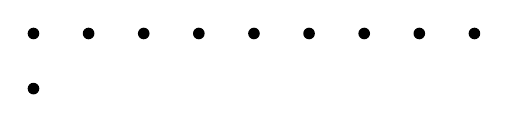
\begin{tikzpicture}[scale=0.7]
	 \fill foreach \Z [count=\Y] in {9, 1}
	  {foreach \X in {1,...,\Z}
	  {(\X,-\Y) circle[radius=3pt]}};

	\end{tikzpicture}\]

	\[\begin{tikzpicture}[scale=0.7]% druga vrstica
	 \fill foreach \Z [count=\Y] in {7, 2, 1}
	  {foreach \X in {1,...,\Z}
	  {(\X,-\Y) circle[radius=3pt]}};

	\end{tikzpicture} \iff  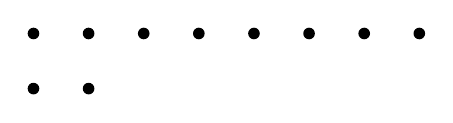
\begin{tikzpicture}[scale=0.7]
	 \fill foreach \Z [count=\Y] in {8, 2}
	  {foreach \X in {1,...,\Z}
	  {(\X,-\Y) circle[radius=3pt]}};

	\end{tikzpicture}\]

	\[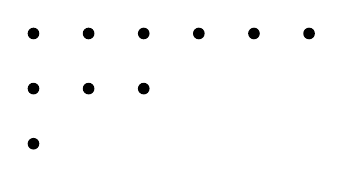
\begin{tikzpicture}[scale=0.7]% tretja vrstica
	 \fill foreach \Z [count=\Y] in {6, 3, 1}
	  {foreach \X in {1,...,\Z}
	  {(\X,-\Y) circle[radius=3pt]}};

	\end{tikzpicture} \iff 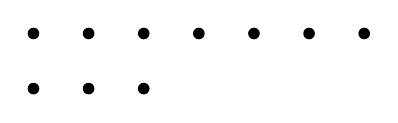
\begin{tikzpicture}[scale=0.7]
	 \fill foreach \Z [count=\Y] in {7, 3}
	  {foreach \X in {1,...,\Z}
	  {(\X,-\Y) circle[radius=3pt]}};

	\end{tikzpicture}\]

	\[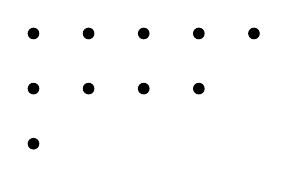
\begin{tikzpicture}[scale=0.7]% "cetrta vrstica
	 \fill foreach \Z [count=\Y] in {5, 4, 1}
	  {foreach \X in {1,...,\Z}
	  {(\X,-\Y) circle[radius=3pt]}};

	\end{tikzpicture} \iff  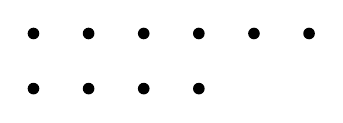
\begin{tikzpicture}[scale=0.7]
	 \fill foreach \Z [count=\Y] in {6, 4}
	  {foreach \X in {1,...,\Z}
	  {(\X,-\Y) circle[radius=3pt]}};

	\end{tikzpicture}\]

	\[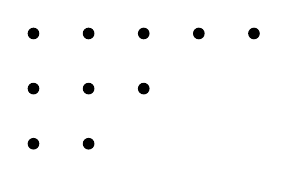
\begin{tikzpicture}[scale=0.7]% peta vrstica
	 \fill foreach \Z [count=\Y] in {5, 3, 2}
	  {foreach \X in {1,...,\Z}
	  {(\X,-\Y) circle[radius=3pt]}};

	\end{tikzpicture} \iff 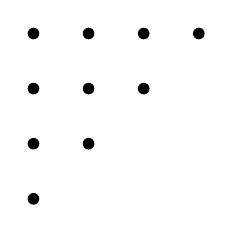
\begin{tikzpicture}[scale=0.7]
	 \fill foreach \Z [count=\Y] in {4, 3, 2, 1}
	  {foreach \X in {1,...,\Z}
	  {(\X,-\Y) circle[radius=3pt]}};

	\end{tikzpicture}\]

	s($\lambda$) $\coloneqq$ $\lambda_{l(\lambda)}$ najmanj"si "clen
	\[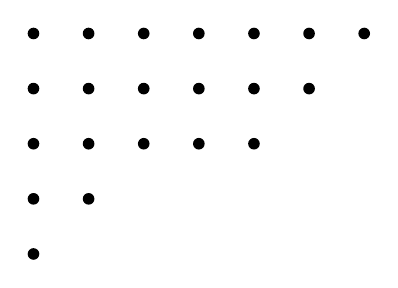
\begin{tikzpicture}[scale=0.7]
	 \fill foreach \Z [count=\Y] in {7, 6, 5, 2, 1}
	  {foreach \X in {1,...,\Z}
	  {(\X,-\Y) circle[radius=3pt]}};
	\end{tikzpicture}\]
	Recimo diagonali, ki se pojavi ob koncu prvih treh vrstic, \textbf{bok}.\\
	\[b(\lambda) \coloneqq \max\{i: \lambda_i = \lambda_1 - i + 1\}\]

	\begin{enumerate}
	    \item "Ce je $s(\lambda) > b(\lambda)$: bok postavimo pod najmanj"si "clen
	    \item "Ce je $s(\lambda) \leqslant b(\lambda)$: najmanj"si "clen postavimo desno od boka
	\end{enumerate}

	Zakaj to ni vselej bijekcija? \label{TODO: add image 5} Prvo pravilo ne deluje, "ce
	\[b(\lambda) = l(\lambda) = s(\lambda) - 1 = k\]
	% Dodaj sliko
	\label{TODO: add image 6}
	\[(k + 1) + (k + 2) + \cdots + (k + k) =\]
	\[\frac{2k (2k + 1)}{2} - \frac{k (k + 1)}{2} = \frac{k (3k + 1)}{2}\]
	Drugo pravilo ne deluje, "ce
	\[b(\lambda) = l(\lambda) = s(\lambda) = k\]
	% Dodaj sliko
	\label{TODO: add image 7}
	\[k + (k + 1) + (k + 2) + \cdots + (k + k - 1) =\]
	\[\frac{(2k - 1) 2k}{2} - \frac{(k - 1) k}{2} = \frac{k (3k - 1)}{2}\]

	\begin{itemize}
	    \item "ce m $\neq$ $\frac{k \cdot (3k \pm 1)}{2}$, smo na"sli bijekcijo, $\alpha(m) - \beta(m) = 0$.
	    \item "ce m = $\frac{k \cdot (3k \pm 1)}{2}$, imamo bijekcijo, "ce odstavimo eno raz"clenitev s $k$ "cleni.
	    \begin{itemize}
	    	\item[*] $k$ sod: $\alpha(m) - \beta(m) = -1$
		    \item[*] $k$ lih: $\alpha(m) - \beta(m) = 1$
		\end{itemize}
	    Torej: $\alpha(m) - \beta(m) = (-1)^{k - 1}$
	\end{itemize}
\end{proof}
\label{TODO: add image 8}
%OPOMBA: (dodaj sliko petkotnikov)\\

\subsection{Dvanajstera pot}
Imamo $n = |N|$ kroglic in $k = |K|$ "skatel. Zanimajo nas razporeditve teh kroglic v "skatle, glede na to ali kroglice in "skatle med seboj lo"cimo ali ne.

Spomnimo se na definiciji injektivnosti in surjektivnosti
\begin{itemize}
    \item injektivna razporeditev: v vsaki "skatli je najve"c ena kroglica
    \item surjektivna razporeditev: v vsaki "skatli je vsaj ena kroglica
\end{itemize}
\[\begin{tabular}{c|c|c c c}
    $N$ & $K$ & vse & injektivne & surjektivne \\
\hline
    Lo"cimo & Lo"cimo & $k^n$ & $k^{\underline{n}}$ & $k!\cdot s(n, k)$\\
    Ne lo"cimo & Lo"cimo & $\binom{n + k - 1}{k - 1}$ & $\binom{k}{n}$ & $\binom{n - 1}{k - 1}$\\
    Lo"cimo & Ne lo"cimo & $\sum_{i \leqslant k} s(n, i)$ & $k \geqslant n \ ? \ 1 : 0$ & $s(n, k)$\\
    Ne lo"cimo & Ne lo"cimo & $\overline{p_k}(n)$ & $k \geqslant n \ ? \ 1:0$ & $p_k(n)$ \\
\end{tabular}\]


% 16. 11. 2021

% honestly, tega pomojem ne rabimo. Je samo confusing
%\begin{ex}
%	Podajmo primer interpretacije po vrsticah.
%
%	1. vrstica: "steje preslikave $[n] \rightarrow [k]$\\
%	2. vrstica: $f, g: \{1, 2, 3\} \rightarrow \{a, b, c, d\}$
%	\[f: \frac{1, 2}{a} \ \frac{}{b} \ \frac{3}{c} \ \frac{}{d}\]
%	\[g: \frac{1, 3}{a} \ \frac{}{b} \ \frac{2}{c} \ \frac{}{d}\]
%	\[\text{Velja, da sta $f \sim_N g$ za ekvivalen"cno relacijo:}\]
%	\[f \sim_N g \text{, "ce $\exists$ } \pi \in S(n)\text{, da je f = g} \circ \pi\]
%	3. vrstica: $f \sim_K g$, "ce $\exists$ $\sigma$ $\in$ S(K), $f = \sigma \circ g$\\
%	4. vrstica: $f \sim_{N, K} g$, "ce $\exists$ $\pi$ $\in$ S(N), $\exists$ $\sigma$ $\in$ S(K), $f = \sigma \circ g \circ \pi$\\
%\end{ex}

\section{Rodovne funkcije}
\subsection{Uvod}
Na kak"sne na"cine lahko predstavimo zaporedje?
\begin{enumerate}
    \item Z eksplicitno formulo
    \[\begin{tabular}{c c c}
    $a_n = 2^n$ & $b_n = n!$ & $F_n = \frac{1}{\sqrt{5}}((\frac{1 + \sqrt{5}}{2})^{n + 1} - (\frac{1 - \sqrt{5}}{2})^{n + 1})$
    \end{tabular}\]
    \item Z rekurzivno zvezo
    \[a_n = F_{n \geqslant d} (a_{n - 1}, a_{n - 2}, ...)\text{ + za"cetni "cleni }a_0, ... a_{d - 1}\]

    \[a_n = 2a_{n-1}, \quad a_0 = 1\]
    \[b_n = nb_{n - 1}, \quad n \geqslant 1, \quad b_0 = 1\]
    \[F_n = F_{n - 1} + F_{n - 2}, \quad n \geqslant 2, \quad F_0 = 1, \quad F_1 = 1\]

    \item Z asimptotsko formulo
    \[F_n \sim \frac{1}{\sqrt{5}}(\frac{1 + \sqrt{5}}{2})^{n + 1}\]
    \[n! \sim \sqrt{2 \pi n}(\frac{n}{e})^n\]
    \begin{defn}[Asimptotska enakost]
    	$a_n \sim b_n \coloneqq \lim_{n \to \infty} \frac{a_n}{b_n} = 1$
    \end{defn}
    \begin{rem}
    	$\sqrt{2 \pi n}(\frac{n}{e})^n$ smatramo za preprostej"so formulo kot $n!$, saj je prej"snja bolj uporabna pri ra"cunanju.
    \end{rem}
	Za izra"cun potence $a^b$ potrebujemo $log_2(b)$ operacij, ra"cunanje $n!$ pa je izjemno po"casno.
	\begin{ex}
		$2^{64} = (((((2^2)^2)^2)^2)^2)^2$
	\end{ex}
	\begin{ex}
		$2^{100} = ((2^{24} \cdot 2)^2)^2$
	\end{ex}
    Ponavadi zaporedja poenostavimo tako, da jih ocenimo s pribi"zkom, ki ima splo"sni "clen oblike $a_n \sim A n^B C^n$.

    \item Z rodovno funkcijo

    Spomnimo se iz analize: $\sum_{n = 0}^{\infty} a_n x^n$ je poten"cna vrsta, ki konvergira na $x \in (-R, R)$, divergira pa na $x \in (-\infty, -R) \cup (R, \infty)$, kjer je $R \in [0, \infty]$ (lahko je tudi $\infty$) konvergen"cni polmer. V $x = \pm R$ ne moremo zagotovo trditi ni"cesar.
    \[R = \lim_{n \to \infty} |\frac{a_n}{a_{n + 1}}| \text{, "ce limita obstaja}\]
    \[R = \frac{1}{\limsup\limits_{n \to \infty} \sqrt[n]{|a_n|}} \in [0, \infty]\]
    Za $\sum_{n = 0}^{\infty} a_n z^n$, z $\in$ $\C$ velja podobno: konvergira za $|z| < R$, divergira za $|z| > R$.
    \begin{ex}
    	$\sum_{n = 0}^{\infty} 2^n x^n$, $R = \lim_{n \to \infty} (\frac{2^n}{2^{n + 1}}) = \frac{1}{2}$, $\frac{1}{\limsup\limits_{n \to \infty} \sqrt[n]{|2^n|}} = \frac{1}{2}$
    \end{ex}
    \begin{ex}
    	$\sum_{n = 0}^{\infty} n! x^n$, $R = \lim_{n \to \infty} (\frac{n!}{(n + 1)!}) = 0$, divergira za $x \neq 0$
    \end{ex}
    \begin{ex}
    	$e^x = \sum_{n = 0}^{\infty} \frac{1}{n!} x^n$
    \end{ex}

    Vzemimo sedaj zaporedje $a_n = 2^n = 1, 2, 4, 8, \ldots$ in ga zapi"simo kot polinom, nato pa uporabimo formulo za poten"cno vrsto.
    \[1 + 2x + 4x^2 + 8x^3 + \cdots = \sum_{n=0}^{\infty} 2^n x^n = \frac{1}{1 - 2x}, \quad |x| < \frac{1}{2}\]
    Zaporedje lahko na ta na"cin ``zakodiramo'' v funkcijo.
    \[a_n = n! \rightarrow \sum_{n = 0}^{\infty} n! \cdot x^n\]
    Ampak tega (za primer $a_n = n!$) "zal ne znamo izra"cunati. Zato bomo vpeljali eksponentno rodovno funkcijo.

    \begin{itemize}
        \item $\sum_{n = 0}^{\infty} a_n \cdot x^n$ je (obi"cajna) rodovna funkcija $(a_n)_n$
        \item $\sum_{n = 0}^{\infty} a_n \cdot \frac{x^n}{n!}$ je eksponentna rodovna funkcija $(a_n)_n$
    \end{itemize}
    \[\sum_{n = 0}^{\infty} n! \cdot \frac{x^n}{n!} = \sum_{n = 0}^{\infty} x^n = \frac{1}{1 - x}\]
    \[\sum_{n = 0}^{\infty} 2^n \cdot \frac{x^n}{n!} = e^{2x}\]
    \[\sum_{n = 0}^{\infty} F_n \cdot x^n = \frac{1}{1-x-x^2}\]
    Zadnji primer bomo izpeljali kasneje.
\end{enumerate}

\subsection{Formalne poten"cne vrste}
\begin{defn}[Polinom]
	\[\R [x] = \{a_0 + a_1 x + a_2 x^2 + ... + a_n x^n: a_0, ..., a_n \in \R\}\]
\end{defn}
Mno"zica realnih ($\R[x]$) oziroma kompleksnih ($\C[x]$) polinomov tvori polje za se"stevanje in mno"zenje (v resnici tudi $\Q[x]$, $\Z_p[x]$ in ostali obsegi).

\[\sum_{i = 0}^n a_i x^{i} + \sum_{j = 0}^m b_j x^j = \sum_{i = 0}^{max(n, m)}(a_i + b_i)x^{i}\]
\[(a_i = 0: i > n; b_j = 0, j > m)\]

Ker se "zelimo ukvarjati zgolj s poljem polinomov (ne s funkcijami), bomo polinom definirali druga"ce
\begin{defn}[Polinom kot zaporedje]
	\[\R[x] = \{(a_0, a_1, ...): a_i \in \R. \text{ Le kon"cno mnogo }a_i \neq 0\}\]
\end{defn}

$(\R[x], +, \cdot)$ je (neskon"cnorazse"zen) vektorski prostor (za $\cdot$ mno"zenje s skalarjem)

$\R_n[x] = \{a_0 + a_1 x + ... + a_n x^n: a_0, ..., a_n \in \R\}$ (polinomi stopnje $\leqslant n$) je $(n + 1)$-dimenzionalen vektorski prostor. Njegova baza je npr. $1, x, x^2, ..., x^n$, lahko pa tudi $1, x^{\underline{1}}, x^{\underline{2}}, ..., x^{\underline{n}}$ ali $1, x^{\overline{1}}, x^{\overline{2}}, ..., x^{\overline{n}}$. Prehodni matriki bi bili $[c(n, k)]$ in $[S(n, k)]$.
\[
	\sum_k c(n, k) x^n = x^{\overline{n}}
	\qquad
	\sum_k S(n, k) x^{\overline{n}} = x^n
\]

\begin{defn}[Konvolucijsko mno"zenje]
	Produkt polinomov po pravilu ``vsak z vsakim''.
	\[\sum_na_nx^n \cdot \sum_nb_nx^n = \sum_n\big(\sum_{k=0}^n(a_kb_{n-k})\big)x^n\]
\end{defn}
\begin{ex}
	$(a_0 + a_1 x + ... + a_n x^n)(b_0 + b_1 x + ... + b_m x^m) = a_0 b_0 + (a_0 b_1 + a_1 b_0)x + (a_0 b_2 + a_1 b_ 1 + a_2 b_0) x^2 + (a_0 b_3 + a_1 b_2 + a_2 b_1 + a_3 b_0)x^3 + ... + a_n b_m x^{n + m}$
\end{ex}
Koeficienti pri $x^k$ so
\[a_0 b_k + a_1 b_{k - 1} + ... + a_k b_0 = \sum_{i = 0}^k a_i b_{k - i} = \sum_{\substack{i, j \geqslant 0 \\ i + j = k}} a_i b_j\]

$(\R[x], +, \cdot)$ je sedaj komutativen kolobar (kjer je $\cdot$ konvolucijski produkt). $\R[x]$, z vsemi temi operacijami tvori komutativno algebro. Lahko bi za kolobar vzeli tudi $\C([0, 1])$. "Ce vzamemo polinome fiksne stopnje $\R^{n \times n}$, dobimo nekomutativno algebro.

\begin{defn}[Algebra]
	Algebrai"cna struktura $((F, +, \cdot), (V, +, \circ))$ je algebra, "ce je $((F, +, \cdot), (V, +))$ vektorski prostor in $\circ$ produkt med vektorji, za katerega velja distributivnost.
\end{defn}
\begin{defn}[Algebra formalnih poten"cnih vrst]
    $\R[[x]]$ je komutativna algebra zaporedij v $\R$.
    \[\R[[x]] = \{(a_0, a_1, a_2, ...): a_i \in \R\} = \{f: \N \rightarrow \R\} = \R^{\N}\]
	Za operacije
    \[(a_n)_n + (b_n)_n = (a_n + b_n)_n\]
    \[\lambda(a_n)_n = (\lambda a_n)_n \quad \lambda \in \R \]
    \[(a_n)_n (b_n)_n = (\sum_{k = 0}^n a_k b_{n - k})_n\]
\end{defn}
Namesto $(a_n)_n$ ali $a_0, a_1, a_2, \ldots$ pi"semo $\sum_{n = 0}^{\infty} a_n x^n$ oziroma $a_0 + a_1 x + a_2 x^2 + ...$. V tem primeru $x$ ni spremenljivka, $x^n$ ni potenciranje, $\cdot$ ni mno"zenje in $+$ ni se"stevanje, temve"c so samo oznake, da lo"cimo med "cleni.

Z izrazom ``formalna poten"cna vrsta'' se nana"samo na neko zaporedje. ``Rodovna funkcija zaporedja'' (ang. ``generating function'') je v bistvu tudi formalna poten"cna vrsta (torej zaporedje), ampak ponavadi s tem mislimo bolj na zaporedje kot celoto, t.j. na funkcijski zapis, npr. $\frac{1}{1-2x}$.

Enota za mno"zenje je $1 = 1 + 0 x + 0 x^2 + ...$. Velja tudi $(1 + x + x^2 + ...) (1 - x) = 1$, torej je $(1 - x)$ multiplikativni inverz za $(1 + x + x^2 + ...)$. To poznamo kot formulo za poten"cno vrsto.
\[\sum_{n = 0}^{\infty} x^n = \frac{1}{1 - x}\]

\begin{claim}
    $\sum_{n = 0}^{\infty} a_n x^n$ ima inverz za mno"zenje natanko tedaj, ko $a_0 \neq 0$.
\end{claim}

\begin{proof}
    ($\Rightarrow$)
    \[\sum_{n = 0}^{\infty} a_n x^n \cdot \sum_{n = 0}^{\infty} b_n x^n = 1\]
    \begin{align*}
        a_0 b_0 &= 1\\
        a_0 b_1 + a_1 b_0 &= 0\\
        a_0 b_2 + a_1 b_1 + a_2 b_0 &= 0\\
        ... &= 0
    \end{align*}

    ($\Leftarrow$)
    Skonstruirajmo inverz za $\sum_{n = 0}^{\infty} b_n x^n$
    \begin{align*}
        b_0 &= \frac{1}{a_0}\\
        b_1 &= -\frac{a_1 b_0}{a_0}\\
        b_2 &= - \frac{a_1 b_1 + a_2 b_0}{a_0}\\
        &...
    \end{align*}
\end{proof}

Vpeljimo nekaj oznak, ki jih bomo uporabljali v nadaljevanju.
\begin{itemize}
    \item[] $F(x) \coloneqq \sum_{n = 0}^{\infty} a_n x^n$
    \item[] $[x^n]F(x) \coloneqq a_n$ ($n$-ti "clen zaporedja)
    \item[] $F(0) \coloneqq [x^0]F(x)$
    \item[] $(F \cdot G)(0) \coloneqq F(0) \cdot G(0)$
    %\item[] Iz analize: $F'(x) = \lim_{h \to 0} \frac{f(x + h) - f(x)}{h}$
    %\item[] V $\R$[[x]] to ni smiselno
    % zakaj bi omenil, ce ni smiselno?
\end{itemize}

\begin{defn}[Odvod formalne poten"cne vrste]
	Definiramo po zgledu odvajanja polinomov pri analizi.
    \[F(x) = \sum_n a_n x^n \implies F'(x) \coloneqq \sum_n (n + 1) a_{n + 1} x^n\]
    \[(a_0, a_1, a_2, ...) \longmapsto (a_1, 2a_2, 3a_3, ...)\]
\end{defn}

\begin{claim}[Odvod produkta]
	Deluje enako kot pri analizi.
	 \[(F(x) G(x))' = F'(x) G(x) + F(x) G'(x)\]
\end{claim}
\begin{proof}
    Preverimo, da se koeficienti ujemajo pri splo"snem "clenu [$x^n$]. Na levi imamo
    \[(n + 1) (a_0 b_{n + 1} + a_1 b_n + ... + a_{n + 1} b_0)\]
    Na desni pa
    \[a_1 b_n + 2a_2 b_{n - 1} 3a_3 b_{n - 2} + ... + (n + 1) a_{n + 1} b_0+ a_0 (n+1) b_{n+1} + a_1 n b_{n} + a_2 (n-1) b_{n-1} + ... + a_n b_1\]
    kar lahko zapi"semo kot
    \[(0+n+1)(a_0 b_{n+1}) + (1+n)(a_1 b_n) + (2+n-1)(a_2 b_{n-1}) + ... +(n+1)(a_n b_1) + (n+1+0)(a_{n+1} b_0)\]
    Od tod neposredno sledi na"sa formula.
\end{proof}

\begin{defn}
    \[e^{\lambda x} \coloneqq \sum_n \frac{\lambda^n}{n!} x^n\]
\end{defn}
\begin{claim}
	Velja $e^{\lambda x} \cdot e^{\mu x} = e^{(\lambda + \mu) x}$
\end{claim}
\begin{proof}Uporabimo formulo za splo"sni "clen konvolucijskega produkta
    \[
    	e^{\lambda x} \cdot e^{\mu x} =
    	\sum_{k = 0}^{n} \frac{\lambda^k}{k!} \frac{\mu^{n - k}}{(n - k)!}
    	\stackrel{?}{=}
    	\frac{(\lambda + \mu)^n}{n!} =
    	e^{(\lambda + \mu) x}
    \]
    "Ce enakost z vpra"sajem pomno"zimo z $n!$, dobimo
    \[\sum_{k = 0}^{n} \binom{n}{k} \lambda^k \mu^{n - k} = (\lambda + \mu)^{n}\]
    kar pa dr"zi po binomskem izreku.
\end{proof}

\begin{rem}
	Ni nujno, da se omejimo na realne polinome. Tudi $\C$[[x]] in $\Q$[[x]] tvorita algebri. Splo"sneje, vzamemo lahko poljuben $K[[x]]$, kjer je $K$ komutativen obseg,
	$(K, +)$ abelova grupa, $(K \setminus \{0\}, \cdot)$ abelova grupa in med operacijama velja distributivnost. To vklju"cuje tudi kon"cna polja, npr. $\Z_p$, kjer je $p$ pra"stevilo.
	\label{TODO: verify the terminology}
\end{rem}

\begin{theorem}
    Polje velikosti $n$ obstaja natanko tedaj, ko je $n$ potenca pra"stevila ($n = p^k$). Za nek $n$ obstaja samo eno tako polje (do izomorfizma natan"cno).
\end{theorem}

\begin{defn}[Karakteristika]
	Je najmanj"se tako "stevilo $k$, da velja $\underbrace{1 + 1 + \cdots}_{k\text{-krat}} = id$.

	Obseg ima karakteristiko $0$, "ce $1 + 1 + ... + 1 \neq 0$.
\end{defn}
\begin{ex}
	V $\Z_5$ velja $1 + 1 + 1 + 1 + 1 = 0$, torej $\Z_5$ ima karakteristiko $5$.
\end{ex}
\begin{ex}
	$\Q$, $\R$ in $\C$ imajo karakteristiko $0$.
\end{ex}
Kon"cna polja imajo karakteristiko p, "ce so velikosti $p^k$.

V $\Z_5$ za vsa "stevila ve"cja od 5 velja $5! = 6! = ... = 0$.
V obsegu s karakteristiko $> 0$ zato izraz $\frac{1}{n!}$ ni nujno definiran. Zato se omejimo na obsege s karakteristiko $0$.

% 23. 11. 2021
\subsection{Uporaba rodovnih funkcij pri re"sevanju rekurzivnih ena"cb}
\begin{rem}
	Dejanski primeri v tem poglavju niso vklju"ceni.
	\label{TODO: zakaj ne? A so stupid, al jih mormo se dodat?}
\end{rem}

Spomnimo se na dekompozicijo parcialnih ulomkov.
\[\frac{x + 1}{(1-2x)(1-x)} = \frac{A}{1-2x} + \frac{B}{1-x}\]

\begin{rem}[Parcialna dekompozicija z metodo prekrivanja]
	V zgornjem primeru obe strani pomno"zimo z $(1 - 2x)$, nato pa vstavimo $x = \frac{1}{2}$. Ostane samo $A = 3$. Pomno"zimo "se z $(1 - x)$ in vstavimo $x = 1$. Dobimo $B = -2$. Po"zvi"zgamo se na deljenje z ni"c, ker deluje.

	Pozor! Ta metoda deluje samo takrat, ko imamo v imenovalcu samo enostavne ni"cle. "Ce imamo tudi ni"cle vi"sjih stopenj, lahko enostavne ni"cle izra"cunamo z metodo prekrivanja, ostale pa ro"cno.
\end{rem}

Ugotovili smo, da $\frac{x + 1}{(1-2x)(1-x)}$, kar je v bistvu $\frac{3}{1 - 2x} - \frac{2}{1 - x}$ lahko interpretiramo kot $a_n = 3 \cdot 2^n - 2$.

Spomnimo se "se na kvadratno ena"cbo.
\[ax^2 + bx + c = a (x - x_1)(x - x_2), \ x_{1, 2} = \frac{- b \pm \sqrt{b^2 - 4ac}}{2a}\]
Pri kombinatoriki jo bomo nekoliko obrnili.
\[c + bx + ax^2 = c(1 - y_1 x)(1 - y_2 x)\]
$\frac{1}{y_1}$ in $\frac{1}{y_2}$ sta ni"cli na"sega polinoma $c + bx + ax^2$.
\[c + b\frac{1}{y} + a\frac{1}{y^2} = 0 \quad / \cdot y^2\]
\[a + by + cy^2 = 0\]
$y_{1, 2}$ sta torej ni"cli obratnega polinoma.

\begin{claim}
    \[\frac{1}{(1 - x)^k} = \sum_{n = 0}^{\infty} \binom{n + k - 1}{k - 1} x^n\]
    \label{produkt_enostavnih_vrst}
\end{claim}

\begin{proof}
    \[\frac{1}{1 - x} \cdot \frac{1}{1 - x} \cdot \cdots \cdot \frac{1}{1 - x} = (1 + x + x^2 + \cdots)(1 + x + x^2 + \cdots)\cdots(1 + x + x^2 + \cdots)\]
    Tako na levi kot na desni strani je $k$ "clenov.
    Vzemimo za primer $k = 3$ in analizirajmo "clen [$x^5$]:
    \[x^5 \cdot x^0 \cdot x^0, \quad x^3 \cdot x^1 \cdot x^1,\quad x^1 \cdot x^2 \cdot x^2, \quad \ldots \]
    Ugotovimo, da delamo "sibke kompozicije mo"ci $k$, teh pa je ravno $\binom{n + k - 1}{k - 1}$.
\end{proof}

\begin{proof}(Z indukcijo)
    Dokaz z indukcijo je bralcu prepu"s"cen za vajo.
\end{proof}

\begin{ex}
	$\frac{1}{1 - x} = \sum_n x^n$.
\end{ex}
\begin{ex}
	$\frac{1}{(1 - x)^2} = \sum_n (n + 1)x^n$.
\end{ex}
\begin{ex}
	$\frac{1}{(1 - x)^3} = \sum_n \binom{n + 2}{2} x^n$.
\end{ex}

\subsubsection{Fibonaccijeva rodovna funkcija}
Poskusimo sestaviti rodovno funkcijo za Fibonaccijevo zaporedje $1, 1, 2, 3, 5, 8, \ldots$. Uporabili bomo oznaki $F_n = n$-ti "clen Fibonaccijevega zaporedja in $F(x) = \sum_{k = 0}^\infty F_n \cdot x^n$, t.j. Fibonaccijeva formalna poten"cna vrsta.
\begin{align*}
	F_n&: 1, 1, 2, 3, 5, 8, 13, 21, \ldots \\
	F_{n-1}&: 0, 1, 1, 2, 3, 5, \ 8, 13, \ldots = x \cdot F(x)\\
	F_{n-2}&: 0, 0, 1, 1, 2, 3, \ 5, \ 8, \ldots = x^2 \cdot F(x)
\end{align*}
Opazimo, da velja $F(x) = 1 + x\cdot F(x) + x^2 \cdot F(x)$. "Ce ta izraz malo uredimo, dobimo
\[F(x)(1 - x - x^2) = 1\]
\[F(x) = \frac{1}{1-x-x^2}\]
Kar je rodovna funkcija za Fibonaccijevo zaporedje.
\label{TODO: izpeljava eksplicitne formule}
\begin{ex}
	$a_n = 2a_{n-1}$, $a_0 = 1$. Pomno"zimo rekurzivno formulo z $x^n$ in se"stejmo $\sum_{n=1}^\infty$.
	\[\sum_{n=1}^\infty a_n x^n = \sum_{n=1}^\infty 2a_{n-1}x^n\]
	Leva stran je $F(x)-1$, ker se"stevamo od $n=1$ namesto od $n=0$. Na desni strani nesemo pred vsoto $2$ in izpostavimo en $x$, da imamo pri $a$ isto "stevilko.
	\[F(x)-1 = 2x\sum_{n=1}^\infty a_{n-1}x^{n-1}=2x\sum_{n=0}^\infty a_{n}x^{n} = 2xF(x)\]
	Izpostavimo $F(x)$ kot prej
	\[F(x)(1-2x)=1 \implies F(x)=\frac{1}{1-2x}\]
	"Ce "zelimo, lahko to pretvorimo "se v eksplicitno formulo.
	\[F(x) = \frac{1}{1-2x} = \sum_{n=0}^\infty 2^nx^n \implies a_n = 2^n\]
\end{ex}

\begin{ex}
	$a_n = 3a_{n-1}-2a_{n-2}$, $a_0 = 1$, $a_1 = 4$. Primer je prepu"s"cen bralcu. Re"sitev je $F(x) = \frac{1+x}{1-3x+2x^2}$ oziroma $a_n = 3\cdot2^n-2$
\end{ex}

Poskusimo posplo"siti zgornji postopek za poljubno homogeno linearno rekurzivno ena"cbo.
\begin{theorem}[Recept za re"sevanje homogene linearne rekurzivne ena"cbe s konstantnimi koeficienti]
    \[c_d a_n + c_{d - 1} a_{n - 1} + \cdots + c_0 a_{n - d} = 0 \ \ \ n \geqslant d\]
    Zapi"simo karakteristi"cni polinom
    \[c_d \lambda^d + c_{d - 1} \lambda^{d - 1} + \cdots + c_0 \ \ \ (c_d, c_0 \neq 0, c_i \in \C)\]
    kjer so $\lambda_1,\ldots, \lambda_k$ ni"cle z ve"ckratnostmi $\alpha_1, \ldots \alpha_k$.
    \[a_n = \sum_{i = 1}^k p_i (n) \lambda_i^n, \quad deg (p_i) < \alpha_i\]
    \label{TODO: kaj je ta izrek? mal sm probu preuredit, ampak sm ugotovu da ne razumm. Also nism pregledu dokaza}
    % a lahko dobimo se en example uporabe tega?
\end{theorem}

\begin{proof}
	Pomno"zimo vrsto z $x^n$ in se"stejmo od $d$ do $\infty$.
    \[c_d a_n + c_{d - 1} a_{n - 1} + \cdots + c_0 a_{n - d} = 0 \ \ \ / x^n / \sum_{n = d}^{\infty}\]
    \begin{align*}
        0 = \ & c_d(F(x) - a_0 - a_1x - \cdots - a_{d - 3}x^{d - 3} - a_{d - 2}x^{d - 2} - a_{d - 1}x^{d - 1})\\
        +\ & c_{d - 1} x (F(x) - a_0 - a_1x - \cdots - a_{d - 3}x^{d - 3} - a_{d - 2}x^{d - 2})\\
        +\ & c_{d - 2} x^2 (F(x) - a_0 - a_1x - \cdots - a_{d - 3}x^{d - 3})\\
        +\ & \cdots \\
        +\ & c_1 x^{d - 1} (F(x) - a_0) \\
        +\ & c_0 x^d F(x)
    \end{align*}
    \[F(x) (c_d + c_{d - 1} x + c_{d - 2} x^2 + \cdots + c_1 x^{d - 1} + c_0 x^d) = P(x) \text{ polinom stopnje < d}\]
    \[F(x) = \frac{P(x)}{c_d + c_{d - 1} x + c_{d - 2} x^2 + \cdots + c_1 x^{d - 1} + c_0 x^d}\]
    Karakteristi"cni polinom: $c_d \lambda^d + c_{d - 1} + \lambda^{d - 1} + \cdots + c_0$ z ni"clami $\lambda_1, \ldots, \lambda_k$
    \begin{align*}
        F(x) & = \frac{P(x)}{c_d \prod_{i = 1}^k (1 - \lambda_i x)^{\alpha_i}} = \\
        & = \sum_{i = 1}^k \sum_{j = 1}^{\alpha_i} \frac{A_{i, j}}{(1 - \lambda_i x)^j} = \\
        & = \sum_{i = 1}^k \sum_{j = 1}^{\alpha_i} A_{i j} \sum_{n = 0}^{\infty} \binom{n + j - 1}{j - 1} \lambda_i^n x^n
    \end{align*}
    \[a_n = \sum_{i = 1}^k (\sum_{j = 1}^{\alpha_i} A_{i j} \binom{n + j - 1}{j - 1})\lambda_i^n = \sum_{i = 1}^k p_i(n)\lambda_i^n\]
    \[\binom{n  j - 1}{j - 1} = \frac{(n + j - 1)(n + j - 2) ... (n + 1)}{(j + 1)!}\]
    \[\text{ polinom stopnje (j - 1)} \implies deg(p_i) < \alpha_i\]
\end{proof}

\begin{theorem}[Re"sevanje nekaterih nehomogenih rekurzivnih ena"cb]
    \[c_d a_n + c_{d - 1} a_{n - 1} + ... + c_0 a_{n - d} = q(n) \lambda^n\]
    Re"sitev je vsota re"sitve homogene ena"cbe in partikularne re"sitve, ki jo poi"s"cemo z nastavkom
    \[a_n = n^{\alpha} r(n) \lambda^n\]
    $\deg(r(n)) \leqslant \deg(q)$, $\alpha$-kratnost $\lambda$ v karakteristi"cnem polinomu,
    \[\alpha \geqslant 0, \quad \alpha = 0 \iff \lambda \text{ ni ni"cla}\]
\end{theorem}

\begin{proof}
    Prepu"s"cen bralcu.
\end{proof}


% 30. 11. 2021
\subsection{Binomska vrsta}
Spomnimo se biomskega koeficienta za $n, k \in \N$
\[\binom{n}{k} = \bigg|\binom{[n]}{k}\bigg| = \frac{n^{\underline{k}}}{k} = \begin{cases}\frac{n!}{k!(n-k)!}: 0 \leqslant k \leqslant n \\ 0: k > n\end{cases}\] %\frac{n \cdot (n - 1) \cdot ... \cdot (n - k + 1)}{k!}\]
\begin{defn}[Posplo"seni binomski koeficient]
	Zahtevamo samo $n \in \N$.
	\[\binom{\lambda}{n} = \frac{\lambda^{\underline{n}}}{n!} = \frac{\lambda \cdot (\lambda - 1) \cdots (\lambda - n + 1)}{n!}\]
	Kjer je $\lambda \in K$, $K$ konvergentni obseg s karakteristiko $0$, npr $\R^2$ ali $\C^2$.
\end{defn}
%Nekaj primerov:
\begin{ex}
	$\binom{\frac{5}{2}}{3} = \frac{\frac{5}{2} \cdot \frac{3}{2} \cdot \frac{1}{2}}{6} = \frac{5}{16}$
\end{ex}
\begin{ex}
	$\binom{i}{2} = \frac{i (i - 1)}{2} = \frac{-1 -i}{2}$
\end{ex}
\begin{ex}
	$\binom{-1}{n} \frac{(-1)(-2)...(-n)}{n!} = (-1)^n$
\end{ex}
\begin{ex}
	$k \in \N$:
	\[\binom{-k}{n} = \frac{-k (-k - 1) ... (-k - n + 1)}{n!} = \frac{(-1)^n (n + k - 1) ... (k + 1) k}{n!} \cdot \frac{(k - 1)!}{(k - 1)!} = \]
	\[ = \frac{(-1)^n (n+l+k-1)!}{n! (k - 1)!} = (-1)^n \binom{n + k - 1}{k - 1}\]
\end{ex}
\begin{ex}
	\[\binom{\frac{1}{2}}{n} = \frac{\frac{1}{2}\cdot(-\frac{1}{2})\cdot(-\frac{3}{2})\cdots(\frac{1}{2}-n+1)}{n!}=\frac{(-1)^{n-1}\cdot1\cdot3\cdot5\cdots(2n-3)}{2^n\cdot n!}\]
	Uporabimo simbol $!!$. Velja $7!! = 1\cdot3\cdot5\cdot7$ oziroma za soda "stevila: $6!! = 2\cdot4\cdot6$. Pri sodih "stevilih pa lahko izpostavimo $2$, da dobimo $6!! = 2^3 \cdot 3!$.
	\[\frac{(-1)^{n-1}(2n-3)!!}{2^n\cdot n!}\cdot\frac{(2n-2)!!}{(2n-2)!!} =
	\frac{(-1)^{n-1}(2n-2)!}{2^n \cdot n!\cdot 2^{n-1}(n-1)!} = \frac{(-1)^{n-1}}{2^{2n-1}\cdot n}\binom{2n-2}{n-1}\]
	"Ce smo malo previdni, opazimo, da to deluje samo pod pogojem $n \geqslant 1$, sicer je $\binom{\frac{1}{2}}{n} = 0$.
\end{ex}

\begin{defn}[Binomska vrsta]
	Naj bo $K$ obseg in $\lambda \in K$.
	\[B_{\lambda} (x) = \sum_{n = 0}^{\infty} \binom{\lambda}{n} x^n\]
	\[= 1 + \lambda x + \frac{\lambda (\lambda - 1)}{2} x^2 + \frac{\lambda (\lambda - 1) (\lambda - 2)}{6} x^3 + ...\]
\end{defn}

\begin{rem}
	Zapis $B_{\lambda}(x)=\sum_{n = 0} \binom{\lambda}{n} x^n$ je napa"cen! Lahko je bodisi $\sum_{n \in \N_0}$, $\sum_{n = 0}^{\infty}$ ali $\sum_{n = 0}^{\lambda}$.
\end{rem}

\begin{ex}
	"Ce za $\lambda$ vzamemo $n \in \N$, dobimo binomski izrek.
	\[B_n (x) = \sum_{k = 0}^{\infty} \binom{n}{k} x^k = \sum_{k = 0}^n \binom{n}{k} x^k = (1 + x)^n\]
\end{ex}

\begin{ex}
	"Ce za $\lambda$ vzamemo $-k$, $k \in \N$, dobimo
	\[B_{-k} (x) = \sum_{n = 0}^{\infty} \binom{-k}{n} x^n = \sum_{n = 0}^{\infty} (-1)^n \binom{n + k - 1}{k - 1} x^n = (1 + x)^{-k}\]
	Zadnjo enakost smo dokazali v prej"snjem razdelku (glej \ref{produkt_enostavnih_vrst}).
\end{ex}

Opazimo o"citen vzorec. Ali bi lahko posplo"sili pravilo $B_{\lambda}(x) = (1 + x)^{\lambda}$? Natan"cneje, "ce bi definirali npr. $(1 + x)^{\frac{1}{2}}$ tako, da velja $((1 + x)^{\frac{1}{2}})^2 = 1$, ali lahko pri"cakujemo, da je $B_{\frac{1}{2}} = (1+x)^{\frac{1}{2}}$? Vse to in "se ve"c bomo lahko trdili, ko doka"zemo $B_{\lambda} (x) \cdot B_{\mu} (x) = B_{\lambda + \mu} (x)$.

\begin{lemma}[Binomski izrek s "crtico]
	\[(a+b)^{\overline{n}} = \sum_{k=0}^n \binom{n}{k}a^{\overline{n-k}} b^{\overline{k}}\]
	\[(a+b)^{\underline{n}} = \sum_{k=0}^n \binom{n}{k}a^{\underline{n-k}} b^{\underline{k}}\]
\end{lemma}
\begin{proof}
    Z indukcijo.\\
    Baza indukcije: $n = 0$, $1 = 1$ $\checkmark$\\
    Indukcijski korak: $n - 1 \implies n$
    \begin{align*}
        (\lambda + \mu)^{\underline{n}} & = (\lambda + \mu)^{\underline{n - 1}}(\lambda + \mu - n + 1) =\\
        & \overset{IP}{=} \sum_k \binom{n - 1}{k} \lambda^{\underline{k}} \mu^{\underline{n - 1 - k}} (\lambda - k + \mu + k - n + 1) = \\
        & = \sum_k \binom{n - 1}{k} \lambda^{\underline{k + 1}} \mu^{\underline{n - 1 - k}} + \sum_k \binom{n - 1}{k} \lambda^{\underline{k}} \mu^{\underline{n - k}} =\\
        & = \sum_k \binom{n - 1}{k - 1} \lambda^{\underline{k}} \mu^{\underline{n - k}} + \sum_k \binom{n - 1}{k} \lambda^{\underline{k}} \mu^{\underline{n - k}} = \\
        & = \sum_k \binom{n}{k} \lambda^{\underline{k}} \mu^{\underline{n - k}}
    \end{align*}
	Dokaz za nara"s"cajo"ce potence prepustimo bralcu.
\end{proof}

\label{TODO: tega ni blo lani in ne razumm, tkoda se ne bom s tem ukvarju}
% remove if applicable

%$((1 + x)^{\lambda})' = \lambda (1 + x)^{\lambda - 1}$.
%\begin{proof}
%    \[(n + 1) \binom{\lambda}{n + 1} \overset{?}{=} \lambda \binom{\lambda - 1}{n}\]
%    \[\cancel{(n + 1)} \frac{\lambda^{\underline{n + 1}}}{\cancel{(n + 1)!}} = \lambda \frac{(\lambda - 1)^{\underline{n}}}{\cancel{n!}} \ \ \ \checkmark\]
%\end{proof}

% ZAPISKI S TEH PREDAVANJ BODO KMALU KON"CANI

\label{TODO: again, kaj je to? (commented out)}
%\[\sqrt{1 + x} = \sum_{n = 0}^{\infty} \binom{\frac{1}{2}}{n} x^n = 1 - 2 \sum_{n = 1}^{\infty} \frac{(-1)^n}{2^{2n}n} \binom{2n - 2}{n - 1} x^n\]

\subsubsection{Catalanova "stevila}
\begin{defn}[Catalanovo "stevilo]
	$C_n$ je "stevilo pravilnih postavitev oklepajev na nizu $n+1$ "stevil $\cycle{t_0, t_1, t_2, \ldots, t_n}$.

	Prvih nekaj Catalanovih "stevil (od $n=0$ dalje): $1, 1, 2, 5, 14, 42, \ldots$.
\end{defn}

\begin{tabular}{c c c c c c}
	$n = 0$& $(t_0)$ & & & &\\
	$n = 1$& $(t_0 t_1)$ & & & &\\
	$n = 2$& $(t_0 t_1) t_2$ & $t_0 (t_1 t_2)$ & & &\\
	$n = 3$& $((t_0 t_1) t_2) t_3$  &  $(t_0 t_1) (t_2 t_3)$ & $t_0 (t_1 (t_2 t_3))$ & $(t_0 (t_1 t_2)) t_3$ & $t_0 ((t_1 t_2) t_3)$
\end{tabular}

Poi"s"cimo rekurzivno zvezo za $C_n$. Za rekurzivni korak bomo izbrali lokacijo zadnjega mno"zenja (stik najbolj zunanjih oklepajev).
\begin{ex}
	Pri $((t_0 t_1) t_2) t_3$ je ``zadnje mno"zenje'' med $((t_0 t_1) t_2)$ in $t_3$, pri $(t_0 t_1) (t_2 t_3)$ pa med $(t_0 t_1)$ in $(t_2 t_3)$.
\end{ex}
V splo"snem, $\cycle{t_0 t_1 \ldots t_k} \cdot \cycle{t_{k + 1} \ldots t_{n+1}}$, kjer velja $0 \leqslant k \leqslant n$.
Ostane nam "se izbira oklepajev med $k$ "cleni in $(n+1)-(k+1)=n-k$ "cleni.

\begin{theorem}[Rekurzivna zveza za $C_n$]
	\[C_{n + 1} = \sum_{k = 0}^{n} C_k C_{n - k} \qquad n \geqslant 0\]
\end{theorem}

Ker smo kul matematiki, se ne bomo zadovoljili zgolj z rekurzivno zvezo.

\begin{theorem}[Eksplicitna formula za $C_n$]
	\[C_n = \frac{1}{n + 1} \binom{2n}{n}\]
\end{theorem}
\begin{proof}
	Definirajmo $F(x) = \sum_{n = 0}^{\infty} C_n x^n$.
	Pomno"zimo rekurzijo z $x^{n + 1}$ in se"stejmo "clene $\sum_{n = 0}^{\infty}$, kot smo to po"celi pri linearnih rekurzijah.
	\[\sum_{n = 0}^{\infty} C_{n + 1} x^{n + 1} = \sum_{n = 0}^{\infty} (\sum_{k = 0}^{\infty} C_k x^k) x^{n + 1}\]
	Levo stran izrazimo kot $F(x) - 1$, na desni strani pa opazimo konvolucijo $F(x)$ s samim sabo. Dobimo torej $x F^2(x)$. "Ce enakost preoblikujemo, dobimo $x F^2(x) - F(x) + 1 = 0$.

	Kaj pa zdaj? No, ko vidimo kvadratno ena"cbo, nas ima, da bi jo re"sili. Poskusimo s kvadratno ena"cbo
	\[F(x) = \frac{1 \pm \sqrt{1 - 4x}}{2x}\]
	Sedaj pa se vpra"sajmo, "ce je ta izraz kaj smiseln. "Ce za"cnemo s "clenom $\sqrt{1-4x}$, lahko uporabimo binomsko vrsto.
	\begin{align*}
		\sqrt{1 + x} &= 1 - 2\sum_{n = 1}^{\infty} \frac{(-1)^n}{2^{2n}n} \binom{2n - 2}{n - 1} x^n\\
		\sqrt{1 - 4x} &= 1 - 2\sum_{n = 1}^{\infty} \frac{\cancel{(-1)^n}}{\cancel{2^{2n}}n} \binom{2n - 2}{n - 1} (-4x)^n\\
		&= 1 - 2\sum_{n = 1}^{\infty} \frac{1}{n} \binom{2n - 2}{n - 1} x^n
	\end{align*}
	Nadaljujemo tako, da izra"cunano vstavimo v prvotno ni"clo.
	\[\frac{1 + \sqrt{1 - 4x}}{2x} = \frac{2 - 2\sum_{n = 1}^{\infty} \frac{1}{n} \binom{2n - 2}{n - 1} x^n}{2x} \qquad \notin k[[x]] \]
	To na "zalost ni formalna poten"cna vrsta, saj delimo neko vrsto z $x$-om, ki se ne more izpostaviti.

	Po drugi strani, "ce vzamemo drugo ni"clo, se nam "clen $1$ kraj"sa, ostane pa lepa formalna poten"cna vrsta.
	\[\frac{1 - \sqrt{1 - 4x}}{2x} = \sum_{n = 1}^{\infty} \frac{1}{n} \binom{2n - 2}{n - 1} x^{n - 1}\]
	Ta vrsta tudi re"si na"so kvadratno ena"cbo.
	\[x (\frac{1 - \sqrt{1 - 4x}}{2x})^2 - \frac{1 - \sqrt{1 - 4x}}{2x} + 1 \underset{\sqrt{1 - 4x}^2 = 1 - 4x}{=} 0\]
	Zato je to na"sa re"sitev.
	\[F(x) = \sum_{n = 0}^{\infty} \frac{1}{n + 1} \binom{2n}{n} x^n\]
\end{proof}

\begin{ex}
	$C_3 = \frac{1}{4} \binom{6}{3} = \frac{\cancel{6} \cdot 5 \cdot \cancel{4}}{\cancel{4} \cdot \cancel{6}} = 5$
\end{ex}
\begin{ex}
	$C_5 = \frac{1}{6} \binom{10}{5} = \frac{\overset{\cancel{2}}{\cancel{2}} \cdot \overset{3}{\cancel{9}} \cdot \overset{2}{\cancel{8}} \cdot 7 \cdot \cancel{6}}{\cancel{6} \cdot \cancel{5} \cdot \cancel{4} \cdot \cancel{3} \cdot \cancel{2}} = 42$
\end{ex}

Catalanova "stevila so zelo pogosta v kombinatoriki. Dva primera uporabe sta:
\begin{itemize}
	\item Dyckove poti dol"zine $n$. To so poti od $(0,0)$ do $(2n, 0)$ s koraki diagonalno gor $(1,1)$ in diagonalno dol $(1, -1)$, a nikoli ne grejo pod $x$ os.
	\item Triangulacije $(n + 2)$-kotnika. To pomeni dodajanje diagonal $(n+2)$-kotniku, dokler nimamo samih trikotnikov.
\end{itemize}

\begin{figure}[h!]
	\centering
	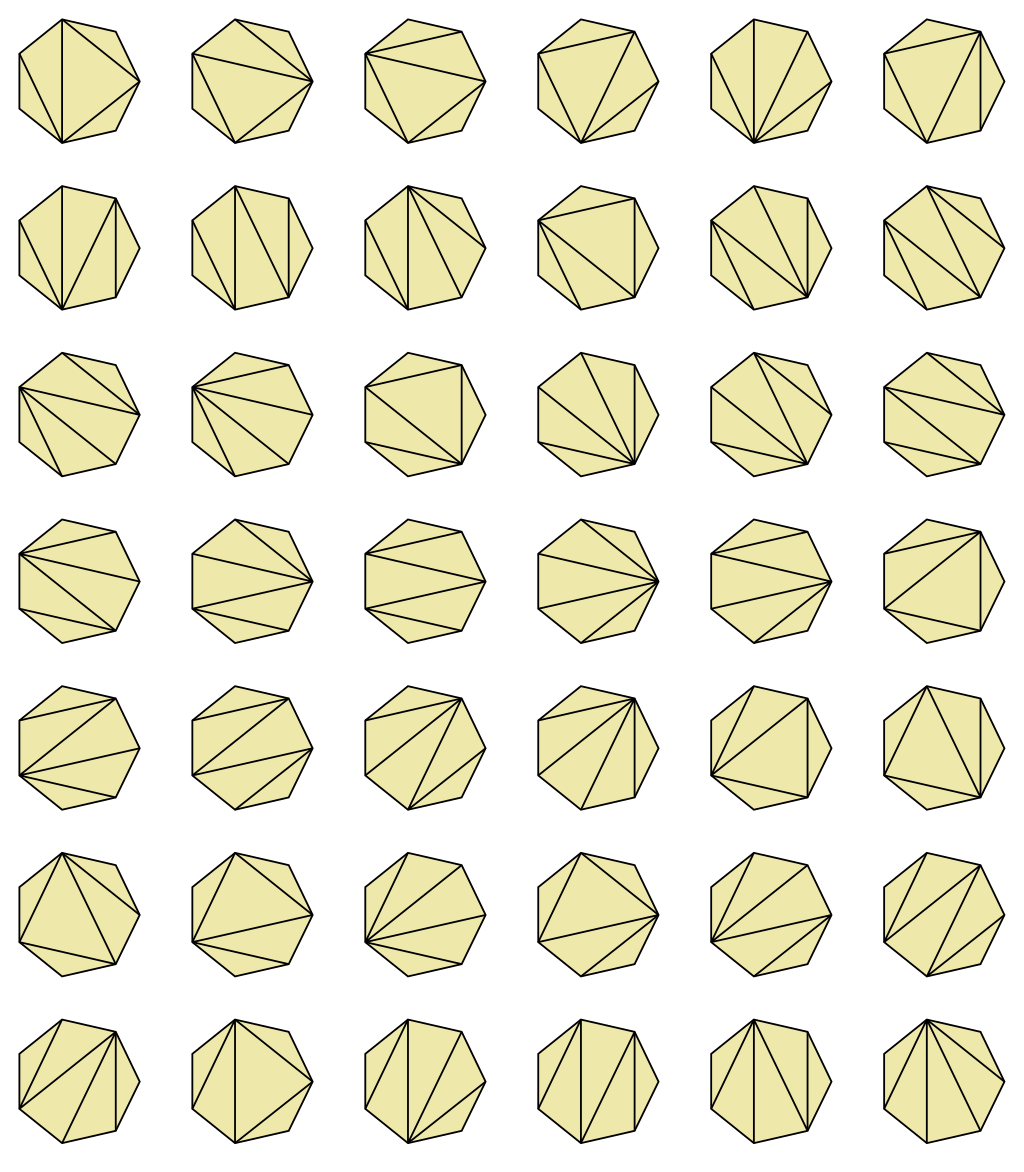
\includegraphics[scale=0.2]{triangulation}
	\caption{Triangulacije sedemkotnika}
\end{figure}
\begin{figure}[h!]
	\centering
	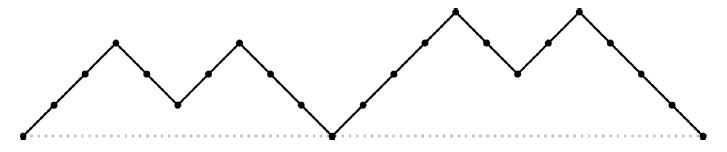
\includegraphics[scale=0.4]{dyck_pic}
	\caption{Dyckova pot}
\end{figure}
Te dve uporabi lahko doka"zete bodisi tako, da najdete bijekcijo med "zelenimi konstrukcijami in postavljanjem oklepajev, bosidi poka"zete, da ima konstrukcija isto rekurzivno zvezo.

V knjigi Enumerative Combinatorics je 66 matemati"cnih struktur, ki jih pre"stevajo Catalanova "stevila. Na spletni strani Richarda Stanlyja jih je "se ve"c kot 100.

\subsection{Rodovne funkcije raz"clenitev}
Spomnimo se na raz"clenitve in "stevila $p_k(n), \overline{p_k}(n), p(n)$.
\begin{ex}
	$n = 5, k = 3: \cycle{3, 2}, \cycle{3, 1, 1}, \cycle{2, 2, 1}, \cycle{2, 1, 1, 1}, \cycle{1, 1, 1, 1, 1}$
\end{ex}

Ugotovili smo "ze, kako izra"cunati koeficient pri $[x^5]$ pri izrazu kot je $(1 + x + x^2 + \ldots)(1 + x + x^2 + \ldots)\ldots$. Kaj pa "ce koeficienti niso povsod enaki?
\[(1 + x + x^2 + \ldots)(1 + x^2 + x^4 + \ldots)(1 + x^3 + x^6 + \ldots) \qquad[x^5]\]
Izberemo nekaj iz prvega oklepaja, pri"stejemo $2\cdot$ nekaj iz drugega in $3 \cdot$ nekaj iz tretjega.
\[x^5 =
x^{0 \cdot 1} \cdot x^{1 \cdot 2} \cdot x^{1 \cdot 3} =
x^{2 \cdot 1} \cdot x^{0 \cdot 2} \cdot x^{1 \cdot 3} =
x^{1 \cdot 1} \cdot x^{2 \cdot 2} \cdot x^{0 \cdot 3} =
x^{3 \cdot 1} \cdot x^{1 \cdot 2} \cdot x^{0 \cdot 3} =
x^{5 \cdot 1} \cdot x^{0 \cdot 2} \cdot x^{0 \cdot 3}\]
To je enak problem, kot "ce bi hoteli zapisati "stevilo $5$ kot vsoto "stevil $1$, $2$ in $3$. Zgoraj bi to izgledalo (z enakim vrstnim redom)
\[5 = 2 + 3 = 1 + 1 + 3 = 1 + 2 + 2 = 1 + 1 + 1 + 2 = 1 + 1 + 1 + 1 + 1\]

\begin{claim}
	\[\sum_{n = 0}^{\infty} \overline{p_k} (n) x^n = \prod_{i = 1}^k \frac{1}{1 - x^i}\]
\end{claim}

\begin{proof}
	Koeficient na obeh straneh je "stevilo re"sitev ena"cbe
	\[a_1 \cdot 1 + a_2 \cdot 2 + \ldots + a_k \cdot k = n\]
	\[\sum_n p_k (n) x^n =  (1 + x + x^2 + \ldots) (1 + x^2+ x^4 + \ldots) \ldots (1 + x^k+ x^{2k} + \ldots)\]
	$p_k (n)$ = "stevilo raz"clenitev $n$ s $k$ "cleni $\leqslant$ $k$, kjer je vsaj en "clen = $k$.
\end{proof}

\begin{claim}
	\[\sum_n p_k(n) x^n = \frac{x^k}{\prod_{i = 1}^k (1 - x^i)}\]
\end{claim}

\begin{claim}
	\[\sum_n p(n) x^n = \prod_{i = 1}^{\infty} \frac{1}{1 - x^i}\]
\end{claim}

\[\text{Pri } [x^n]: (1 + x + x^2 + \ldots) (1 + x^2 + x^4 + \ldots) \ldots (1 + x^n + x^{2n} + \ldots)\underset{\text{ignoriramo}}{(1 + x^{n + 1} + x^{2n + 2} + \ldots) \ldots}\]
\[\implies \overline{p_n}(n) = p(n)\]

\begin{ex}
	$o(n)$ je "stevilo raz"clenitev $n$ s samimi lihimi "cleni
	\[\sum_n o(n) x^n = \prod_{i = 0}^{\infty} \frac{1}{1 - x^{2 i - 1}}\]
\end{ex}
\begin{ex}
	$d(n)$ je "stevilo raz"clenitev $n$ z razli"cnimi "cleni
	\begin{align*}
		\sum_n d(n) x^n &= \prod_{i = 1}^{\infty} (1 + x^i) \cdot \frac{\prod_{i = 1}^{\infty} (1 - x^i)}{\prod_{i = 1}^{\infty} (1 - x^i)}\\
		&= \frac{\prod_{i = 1}^{\infty} (1 - x^{2i})}{\prod_{i = 1}^{\infty} (1 - x^i)}\\
		&= \prod_{i = 1}^{\infty} \frac{1}{1 - x^{2i - 1}}
	\end{align*}
	\[\implies o(n) = d(n)\]
\end{ex}


% 7. 12. 2021
% by Toma"z
\label{TODO: to sm malo spustu}
\subsection{Uporaba rodovnih funkcij}

(1) Rodovna funkcija je pogosto ``lepa'', tudi "ce za zaporedje nimamo ``lepe'' formule.
\begin{ex}
	$\sum_k c(n,k)x^k = x^{\overline{n}}$.
\end{ex}
(2) Rodovno funkcijo se da pogosto zapisati iz kombinatori"cnega problema (ve"c pri kombinatoriki 2).
\begin{ex}
	$i_n \text{ je "stevilo involucij v } S_n \text{, torej } \pi^2 = id$, $\sum i_n \frac{x^n}{n!} = e^{x+\frac{x^2}{2}}$.
	Pomen: $e$ na nekaj sestavljeno iz $x$ (cikli dol"zine 1) in $\frac{x^2}{2}$ (cikli dol"zine 2).
\end{ex}

(3) V rodovni funkciji so ``skriti'' vsi drugi zapisi zaporedja.
\begin{ex}
	$\sum_n F_n x^n = \frac{1}{1-x-x^2} \to (1-x-x^2) \sum_n F_n x^n = 1$.
\end{ex}
\[[x^n]: F_n - F_{n-1} - F_{n-2} = 0 \] \\
asimptotika: vzamemo singularnost ($x_0$), ki je najbli"zje izhodi"s"cu \[F_n \sim An^B(\frac{1}{x_0})^n\] \\
(4) Iz rodovnih funkcij lahko izra"cunamo "se drugo: povpre"cje, varianco $\dots$ \\
npr. koliko elementov ima v povpre"cju podmno"zica $[n]$?
\[\frac{\sum_{S \subseteq [n]} |S|}{2^n} = \frac{\sum_k k \cdot \binom{n}{k}}{2^n} = \frac{n2^{n-1}}{2^n} = \frac{n}{2}\]

% 11. predavanje, 14. 12. 2020
% by Yon, transkripcija lanskih zapiskov
\section{P\'{o}lyeva teorija}
\begin{ex}
	Koliko je ogrlic z $n$ koraldami $k$ barv?
	Dve ogrlici sta enaki, "ce eno iz druge dobimo z rotacijo.
\end{ex}
\begin{ex}
	Koliko je zapestnic z $n$ koraldami $r$ barvami?
	Dve zapestnici sta enaki, "ce eno iz druge dobimo z rotacijo ali zrcaljenjem.
\end{ex}
Nekateri objekti so ekvivalentni, zanima nas "stevilo ekvivaletnih razredov barvanj.

\begin{defn}[Permutacijska grupa]
	je grupa $G \leq S_n$
\end{defn}
\begin{theorem}[Cayleyev]
	Vsaka grupa je izomorfna neki permutacijski grupi.
\end{theorem}
\begin{proof}
	Naj bo $G$ poljubna grupa in $g \in G$. Definirajmo $T_g: G \rightarrow G$:
	\[ T_g(x) = gx \]
	$T_g$ je permutacija mno"zice G. \\
	$H = \lbrace T_g: g \in G \rbrace$ je grupa za komponiranje. \\
	$H \cong G$
\end{proof}
\begin{ex}[Cikli"cna grupa]
	$C_n = \lbrace \cycle{1, 2, 3, \ldots, n}^i: 0 \leq i \le n \rbrace \leq S_n$\\
	$C_n \cong \Z_n$\\
	$\phi: \Z_n \rightarrow C_n := i \rightarrow \cycle{1, 2, \ldots, n}^i$
\end{ex}

\begin{ex}[Diedrska grupa]
	$D_n = \lbrace \text{rotacije + zrcaljenja} \rbrace \leq S_n$\\
	$|D_n| = 2n$ ($n$ zrcaljenj in $n$ rotacij)
	\\
	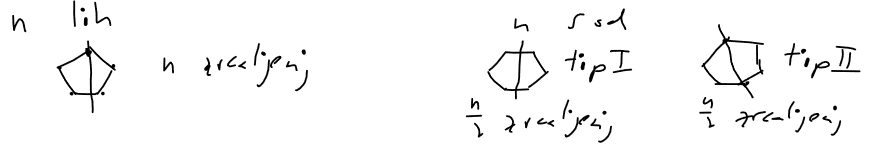
\includegraphics{diedrska}
\end{ex}
\begin{defn}[$x \sim y$]
	$\exists g \in G: g \cdot x = y$
\end{defn}
\begin{claim}
	$\sim$ je ekvivalen"cna relacija.
\end{claim}
$X$ z operacijo $\sim$ razpade na ekvivalen"cne razrede, ki jih imenujemo orbite. Orbito elementa $x$ v $G$ ozna"cimo $Gx$ ($\neq G_x$!!).
\subsection{Orbite, stabilizatorji in negibne to"cke}
\begin{defn}[Orbita]
	$$Gx = {g \cdot x: g \in G}$$
\end{defn}
\begin{rem}
	\label{orbita_neq_odsek}
	Koncept orbit spominja na leve (desne) odseke, a ni isto. Pri odsekih imamo podgrupo, tukaj pa $x$ niti ni element $G$. Pomembna posledica je, da so orbite lahko razli"cno velike, odseki pa so po mo"ci vedno enaki ($|aH|=|bH|$).
\end{rem}
\begin{ex}
	Za $G=C_n, D_n \text{ ali } S_n$ velja $Gx = X$ (samo ena orbita).
\end{ex}
\begin{ex}
	% maybe je +1 thing lih obratno, se mi zdi da je neki menjou kaj je tip 1 in kaj je tip 2
	$$G = \lbrace\text{id, zrcaljenje}\rbrace \leq S_n$$
	$$\text{"stevilo orbit} = \begin{cases}\frac{n+1}{2}; \quad n\text{ lih} \\ \frac{n}{2}; \quad n\text{ sod, zrcaljenje tipa }1 \\ \frac{n}{2}+1; \quad  n\text{ sod, zrcaljenje tipa }2\end{cases}$$
\end{ex}
Mno"zico orbit ozna"cimo z $X/G$.
\begin{rem}
	Na enak na"cin smo ozna"cili tudi faktorske grupe (mno"zice odsekov), a koncept ni isti, ker orbita~$\neq$~odsek (glej opombo \ref{orbita_neq_odsek} pri definiciji orbite).
\end{rem}
\begin{defn}[Stabilizator]
	$$G_x = \lbrace g \in G: g \cdot x = x \rbrace$$
	Elemente $G_x$ ($\neq Gx$!!) imenujemo stabilizatorji $x$-a.
\end{defn}
\begin{defn}[Negibna to"cka]
	$$X_g = \lbrace x \in X: g \cdot x = x \rbrace$$
	Elemente $X_g$ imenujemo negibne to"cke $g$-ja.
\end{defn}
\begin{theorem}
	$$G_x \leq G$$
\end{theorem}
\begin{proof}
	$$id \in G_x$$
	$$g, h \in G_x \implies g \cdot x = x, h \cdot x = x$$
	$$\implies (g \cdot h) \cdot x = g \cdot (g \cdot x) = g \cdot x = x $$
	$$\implies g \cdot h \in G_x$$
	$$g \in G_x \implies g \cdot x = c \implies g^{-1} \cdot x = g^{-1} \cdot g \cdot x = x$$
	$$ \implies g^{-1} \in G_x $$
\end{proof}
\begin{ex}
	$G = C_n$\\
	$G_x = \lbrace id \rbrace$\\
	$X_g = \begin{cases}x: g = id\\\emptyset: g\neq id\end{cases}$
\end{ex}
\begin{ex}
	$G = D_n$\\
	$G_x = \lbrace id, \text{zrcaljenje} \rbrace$\\
	$X_g = \begin{cases}n: g = id\\ 0: (g \text{ rotacija) ali }(g\text{ zrcaljenje tipa 1 in }n\text{ sod}) \\ 1: g \text{ zrcaljenje, }n\text{ lih} \\ 2: g \text{ zrcaljenje tipa 2, }n\text{ sod}\end{cases}$
\end{ex}

\begin{claim}
	$$|G| = |G_x| \cdot |Gx| \quad \forall x \in X$$
\end{claim}
\begin{proof}
	Spomnimo se levih odsekov $\ldots$
	$$ H \leq G \models g \cdot H = \lbrace g \cdot h : h \in H \rbrace \quad \text{je levi odsek v }G $$
	$$g = e \implies g \cdot H = H$$
	$g \cdot H$ in $g' \cdot H$ sta bodisi enaka, bodisi disjunktna.
	$G$ torej razpade na leve odseke, ki imajo enako mo"c ($H \rightarrow gH$ je bijekcija; inverz $g \rightarrow g^{-1}h$).
	\\
	\ldots in kvocientnih mno"zic
	$$G/H = \lbrace gH: g \in G \rbrace$$
	$$|G/H| = \frac{|G|}{|H|} \quad \text{(torej } |H| \text{ deli } |G|\text{)} $$
	Uporabimo za $H=G_x$
	Vemo, da velja $$|G/G_x| = \frac{|G|}{|G_x|}$$
	Definirajmo $$\phi: Gx \rightarrow G/G_x \quad \text{kot} \quad g \cdot x \rightarrow gG_x$$
	$\phi$ je o"citno bijekcija, torej imata $Gx$ in $G/G_x$ enako mo"c.
	Velja torej
	$$|G_x|\cdot|Gx| = |G_x| \cdot |G/G_x| = |G_x| \cdot \frac{|G|}{|G_x|} = |G| $$
	Pozor! $g$ ni enoli"cno dolo"cen. Poka"zimo, da je $\phi$ dobro definirana (za nek vhod dobimo enoli"cen izhod).
	$$g \cdot x = h \cdot x \iff h^{-1} \cdot g \cdot x = x \iff h^{-1} \cdot g \in G_x \iff h^{-1} \cdot g \cdot G_x = G_x \iff g \cdot G_x = h \cdot G_x $$
	Hkrati smo pokazali, da je injektivna (ker so vmes ekvivalence, ne samo implikacije).
	Poka"zimo "se, da je surjektivna:
	$$gG_x = \phi (g \cdot x) $$
	$$\implies |G_x| = \frac{G}{G_x}$$
\end{proof}

\begin{ex}
	Pre"stej simetrije tetraedra.\\
	$|G| = |G_x||Gx| = 3 \cdot 4 = 12$\\
	$\text{id} + \text{rotacije za }120^{\circ} + \text{rotacije za }180^{\circ}$\\
	$1 + 4 \cdot 2 + 3 = 12$
\end{ex}
\begin{ex}
	Pre"stej simetrije kocke.\\
	$|G| = |G_x||Gx| = 3 \cdot 8 = 24$
\end{ex}


% 12. predavanje, 21. 12. 2020
% by Yon, transkripcija lanskih zapiskov
\subsection{Burnsidova lema}
\begin{lemma}[Burnsidova]
	"Stevilo orbit je enako povpre"cnemu "stevilu negibnih to"ck.
	$$|X/G| = \frac{1}{|G|}\sum_{g \in G}|X_g|$$
\end{lemma}
\begin{proof}
	% je to fubinijev izrek?
	$$\sum_{g \in G}|X_g| = \sum_{g \in G}\sum_{x \in X_g}1 = \sum_{g \in G}\sum_{\stackrel{x\in X}{g \cdot x = x}}1 = \sum_{x \in X}\sum_{\stackrel{g \in G}{g \cdot x = x}}1 = \sum_{x \in X}\sum_{g \in G_x}1 = \sum_{x\in X}|G_x|$$
	\begin{rem}
		Ta del bi lahko utemeljili tudi s tabelco: v vrstice napi"semo elemente $X$, v stolpce elemente $G$. Na polju $(g, x)$ naredimo kljukico ntk. $g \cdot x = x$. "Stevilo kljukic po vrsticah je $\sum_{x\in X}|G_x|$, "stevilo kljukic po stolpcih pa $\sum_{g \in G}|X_g|$.
	\end{rem}
	$$\sum_{g \in G}|X_g| = \sum_{x\in X}|G_x| = \sum_{x \in X}\frac{|G|}{|Gx|} = |G| \sum_{x \in X}\frac{1}{|Gx|}$$
	Analizirajmo pomen faktorja $\sum_{x \in X}\frac{1}{|Gx|}$. Za vsak $x$ iz na"se mno"zice vzamemo inverz mo"ci njegove orbite. Ker vsak $x$ pripada natanko eni orbiti, in ker ima vsaka orbita natanko toliko $x$-ov, kolikor je njena mo"c, dobimo slede"co sliko
	$$
	\underbrace{\frac{1}{2}+\frac{1}{2}}_{=1} +
	\underbrace{\frac{1}{1}}_{=1} +
	\underbrace{\frac{1}{4}+\frac{1}{4}+\frac{1}{4}+\frac{1}{4}}_{=1} +
	\ldots
	= \text{"stevilo orbit}
	$$
	oziroma ra"cunsko (oznaka $\sigma =$ orbita)
	$$\sum_{x \in \sigma}\frac{1}{|\sigma|} = |\sigma| \cdot \frac{1}{|\sigma|} = 1$$
	kar lahko uporabimo, da poenostavimo
	$$|G| \sum_{x \in X}\frac{1}{|Gx|} = |G| \sum_{\sigma \in X/G}\sum_{x \in \sigma}\frac{1}{|\sigma|} = |G| \sum_{\sigma \in X/G}1 = |G| \cdot |X/G|$$
\end{proof}
\begin{ex}
	$G=C_n$. $|X/G|$ je o"citno $1$, saj lahko iz ene to"cke z rotacijami v ciklu pridemo kamorkoli, torej imamo samo eno orbito. Ko se"stevamo "stevila negibnih to"ck, ugotovimo, da jih je pri identiteti $n$, pri ostalih $n-1$ ciklih pa nobene.
	$$1 = \frac{1}{n}(n + (n-1)\cdot 0)$$
\end{ex}
\begin{ex}
	$G=D_n$. Spet imamo o"citno samo $1$ orbito. Na desni strani pa "stejemo: $n$ negibnih to"ck pri identiteti, $(n-1)$ pravih rotacij, ki nimajo nobene negibne to"cke, $n$ zrcaljenj z $1$ negibno to"cko "ce je $n$ lih, sicer pa "se $\frac{n}{2}$ zrcaljenj preko simetrale stranic ($0$ negibnih to"ck) in $\frac{n}{2}$ zrcaljenj preko diagonale ($2$ negibni to"cki).
	$$n\text{ lih:} \quad 1 = \frac{1}{2n}(n + (n-1)\cdot 0 + n \cdot 1)$$
	$$n\text{ sod:} \quad 1 = \frac{1}{2n}(n + (n-1)\cdot 0 + \frac{n}{2} \cdot 0 + \frac{n}{2} \cdot 2)$$
\end{ex}
\begin{ex}
	$G = \lbrace \text{id, zrcaljenje} \rbrace$. Lo"cimo primera glede na parnost $n$-ja in tip zrcaljenja.
	$$n\text{ lih, zrcaljenje preko to"cke:}\quad 1 + \frac{n-1}{2} = \frac{1}{2}(n+1)$$
	$$n\text{ sod, zrcaljenje preko to"ck:}\quad 2 + \frac{n-2}{2} = \frac{1}{2}(n+2)$$
	$$n\text{ sod, zrcaljenje preko stranice:}\quad \frac{n}{2} = \frac{1}{2}(n+0)$$
\end{ex}
\begin{ex}
	$G = S_n$.
	$$1 = \frac{1}{n!}\sum_{\pi \in S_n} \# \text{negibnih to"ck }\pi$$
	Ugotovili smo, da je vsota "stevil negibnih to"ck vseh permutacij enaka $n!$. To ni povsem o"citno, ampak lahko sami preverite.
\end{ex}
\begin{ex}
	$3 \times 3$ mre"za z $2$ luknjama. Koliko razli"cnih konfiguracij obstaja, "ce konfiguraciji smatramo za enaki ntk. lahko eno dobimo iz druge z rotacijami in zrcaljenji?
	\\
	Vzemimo za $X$ mno"zico vseh izbir lukenj na plo"s"ci ($|X|=\binom{9}{2}=36$). Na tej mno"zici deluje $D_4$ ($|D_4| = 8$). Pri identiteti imamo torej $36$ negibnih to"ck, pri rotacijah za $90^{\circ}$ vedno $0$, pri rotacijah za $180^{\circ}$ lahko izberemo katerkoli nasprotni par lukenj ($4$ mo"zne izbire), pri vodoravnih in navpi"cnih zrcaljenjih $6 + 6$, pri diagonalnih zrcaljenjih pa "se $2 \cdot 6$ izbir.
	$$\frac{1}{8}(36+0+4+12+12)=8$$
	\begin{rem}
		"Ce tu ne dobimo naravnega "stevila, smo falili.
	\end{rem}
\end{ex}

\subsection{Cikli"cni indeks}
Naj bo $G \leq S_n$ permuatacijska grupa, $n=|X|$.
$g \in G$ je permutacija elementov iz $X$, ki jo seveda lahko enoli"cno zapi"semo $g$ kot produkt disjunktih ciklov.
\begin{defn}[Cikli"cni indeks]
	Ozna"cimo z $\alpha_i(g)$ "stevilo ciklov dol"zine $i$.
	Cikli"cni indeks $Z_G(t_1, \ldots, t_n)$ definiramo kot
	$$ Z_G(t_1, \ldots, t_n) = \frac{1}{|G|}\sum_{g \in G}t_1^{\alpha_1(g)}t_2^{\alpha_2(g)}\cdots t_n^{\alpha_n(g)} $$
\end{defn}
\begin{ex}
	$G=C_4$. $|G|=4$. Za vsak element grupe pogledamo kak"sna je cikli"cna struktura. $id$ ima $4$ cikle dol"zine $1$, torej dobimo "clen $(t_1)^4$. Rotacija za $180^{\circ}$ ima $2$ cikla dol"zine $2$ ($\cycle{1, 2, 3, 4}$ in $\cycle{1, 4, 3, 2}$), torej $(t_2)^2$, vsaka od dveh rotacij za $90^{\circ}$ pa je cikel dol"zine $4$, torej $2 \cdot (t_4)^1$.
	$$Z_{C_4}(t_1, t_2, t_3, t_4) = \frac{1}{4}((t_1)^4+(t_2)^2+2 \cdot t_4)$$
\end{ex}
\begin{ex}
	$G=D_4$. Imamo identiteto, rotacijo za $180^{\circ}$, dve rotaciji za $90^{\circ}$, $4$ zrcaljenja (vodoravno, navpi"cno in dve diagonalni). $Z_{D_4}(t_1, t_2, t_3, t_4) = \frac{1}{8}((t_1)^4+(t_2)^2+2t_4+2(t_2)^2+2(t_1)^2t_2)$.
\end{ex}


\begin{theorem}[Cikli"cni indeks $C_n$]
	\[ Z_{C_n}(t_1, \ldots, t_n) = \frac{1}{n}\sum_{d | n} \phi(d) \cdot (t_{\frac{n}{d}})^d \]
\end{theorem}
\begin{theorem}[Cikli"cni indeks $D_n$]
	\[	Z_{D_n} = \frac{1}{2}Z_{C_n} +
	\begin{cases}
		\frac{1}{2} t_1 t_2^{\frac{n-1}{2}}: n \text{ lih}
		\\
		\frac{1}{4} t_2^{\frac{n}{2}} + \frac{1}{4} t_1^2 t_2^{\frac{n}{2}-1}: n \text{ sod}
	\end{cases}
	\]
\end{theorem}
\begin{rem}[Formula za Eulerjevo funkcijo]
	\[\phi(n) = n \prod_{\mathclap{\substack{p|n \\ p \in \mathbb{P}}}}(1-\frac{1}{p})\]
\end{rem}
\begin{proof}
	Cikli"cna grupa je sestavljena iz dolgega cikla in vseh njegovih potenc. $C_n = \{\cycle{1, \ldots, n}^i: 0 \leqslant i \leqslant n-1 \}$. Kak"snega tipa je dolg cikel na neko potenco?
	
	$\cycle{1, 2, 3, 4, 5, 6}^2 = \cycle{1, 3, 5}\cycle{2, 4, 6}$.
	
	$\cycle{1, 2, 3, 4, 5, 6}^3 = \cycle{1, 4}\cycle{2, 5}\cycle{3, 6}$.
	
	$\cycle{1, 2, 3, 4, 5, 6}^4 = \cycle{1, 5, 3}\cycle{2, 6, 4}$.

	$\cycle{1, 2, 3, 4, 5, 6}^5 = \cycle{1, 6, 5, 4, 3, 2}$.
	
	Opazimo, da velja
	\[d | n \implies \cycle{1, 2, \ldots, n}^d = \cycle{1,\ (d+1),\ (2d+1),\ \ldots \ }\cycle{2,\ (d+2),\ (2d+2),\ \ldots \ }\cdots\]
	Kar pomeni, da je $\cycle{1, 2, \ldots, n}^d$ produkt $d$ ciklov dol"zine $\frac{n}{d}$. Hkrati, "ce $d \perp n$, je $\cycle{1, 2, \ldots, n}^d$ en sam cikel dol"zine $d$.

	Vzemimo $d=\gcd(n, i)$, $n=d\cdot n'$, $i = d \cdot i'$. Vemo, da $\gcd(n', i')=1$. Po prej"snjih ugotovitvah velja
	\[\cycle{1, 2, \ldots, n}^i = (\cycle{1, 2, \ldots, n}^d)^{i'}\]
	Ker je $\cycle{1, 2, \ldots, n}^d$ produkt $d$ ciklov dol"zine $n'$ in ker sta si $n'$ in $i'$ tuji, je rezultat "se vedno produkt $d$ ciklov dol"zine $n'=\frac{n}{d}$. Doprinos k cikli"cnemu indeksu bo $(t_{\frac{n}{d}})^d$. Kolikokrat pa dobimo ta "clen? Tolikokrat, kolikor je $i$-jev, da je $\gcd(n, i)=d$. To nam pove Eulerjeva funkcija $\phi(\frac{n}{d})$.
\end{proof}
\begin{rem}
	$d$ lahko zamenjamo z $\frac{n}{d}$. Dobimo popolnoma ekvivalentno formulo
	\[Z_{C_n}(t_1, \ldots, t_n) = \frac{1}{n}\sum_{d|n}\phi(d) \cdot (t_d)^\frac{n}{d}\]
\end{rem}
\begin{proof}"Se za $D_n$.
	\[
	Z_{D_n} = \frac{1}{2}Z_{C_n} +
	\begin{cases}
		\frac{1}{2} t_1 t_2^{\frac{n-1}{2}}: n \text{ lih}
		\\
		\frac{1}{4} t_2^{\frac{n}{2}} + \frac{1}{4} t_1^2 t_2^{\frac{n}{2}-1}: n \text{ sod}
	\end{cases}
	\]
	Prvi del so rotacije, ki jih je enako kot pri $C_n$ (deliti moramo z $\frac{1}{2}$, ker ima $D_n$ dvakrat ve"c elementov; na za"cetku delimo z $2n$ namesto z $n$). Pri"steti moramo le "se zrcaljenja. 
	
	"Ce je $n$ lih, so vsa zrcaljenja istega tipa. Takih zrcaljenj je $n$. Ko delimo s "stevilom elemenotov ($2n$), je to $\frac{1}{2}$. Doprinos od enega zrcaljenja je $1$ negibna to"cka in $\frac{n-1}{2}$ parov to"ck, ki se izmenjajo.
	
	"Ce je $n$ sod, lo"cimo na $\frac{n}{2}$ zrcaljenj prek to"cke in $\frac{n}{2}$ zrcaljenj prek stranice. Spet delimo "se z $2n$, ostane $\frac{1}{4}$. Pri zrcaljenju "cez simetralo stranic dobimo $\frac{n}{2}$ $2$-ciklov. Pri zrcaljenju "cez to"cki imamo $2$ negibni to"cki, nato pa ostalih $n-2$ ogli"s"c razdelimo v pare.
\end{proof}


\subsection{"Stevilo neekvialentnih barvanj}
V tem razdelku bomo ugotovili pravo uproabnost Burnsidove leme in cikli"cnega indeksa.
\begin{defn}[Barvanje]
	"Ce je $R$ mno"zica barv, je barvanje $b \in R$ preslikava iz mno"zice korald v mno"zico barv
	$b : X \to R$.
	$R^X$ je tedaj mno"zica barvanj.
\end{defn}

Namesto da permutiramo koralde, lahko $G$ razumemo tudi kot grupo permutacij barvanj (podgrupo $S_{R^X}$). Ker je $g$ permutacija korald, moramo posebej definirati, kako uporabimo $g \in G$ na barvnju $b \in R^X$.
\begin{defn}[Permutacija barvanja]
	$g \cdot b(x) \coloneqq b (g^{-1} \cdot x)$
\end{defn}
S tem smo dobili izomorfno permutacijsko grupo. Ne bom bolj natan"cno povedal, kaj s tem mislim.

Nas zanima "stevilo neekvivalentnih barvanj na"se ogrlice. To je ravno "stevilo orbit na"se grupe permutacij barvanj ($G=C_n$ za "stevilo barvanj ogrlic, $G=D_n$ za "stevilo barvanj zapestnic).
Po Burnsidovi lemi moramo izra"cunati povpre"cno "stevilo negibnih to"ck.
\begin{ex}
	$n=6$, $r=2$, $g$ je rotacija za $120^{\circ}$. Koliko je negibnih to"ck za barvanje? Pozor: za permutacijo korald pri taki rotaciji nimamo negibnih to"ck. Mi "stejemo negibne to"cke barvanj. Take negibne to"cke so: barvanje, kjer so vse koralde bele/"crne in barvanje kjer je vsaka druga koralda bela/"crna. Imamo torej $4$ negibne to"cke.
\end{ex}
\begin{ex}
	"Ce bi v prej"snjem primeru vzeli rotacijo za $60^{\circ}$, bi imeli $2$ negibni to"cki. "Ce bi vzeli rotacijo za $180^{\circ}$, bi imeli $8$ negibnih to"ck.
\end{ex}

V splo"snem: i"s"cemo permutacij barvanj, kjer je $b = g \cdot b$, oziroma $g\cdot b(x) = b(g^{-1} \cdot x) = b(x)$ za vsak $x \in X$.
Druga"ce re"ceno, i"s"cemo "stevilo $g$-jev, kjer sta $x$ in $g^{-1}\cdot x$ vedno iste barve. Za vsak tak $g$ velja, da so tudi $gx, g^2x, g^3x, \ldots$ iste barve.

Ugotovimo, da je edina zahteva, da mora biti vsak cikel $g$ v celoti iste barve. Torej je "stevilo negibnih barvanj enako $r^{c(g)}$, kjer je $c(g)$ "stevilo ciklov v $g$, oziroma $c(g) = \displaystyle\sum_i \alpha_i(g)$.

\begin{theorem}[P\'{o}lyev izrek]
	"Stevilo neekvivalentnih barvanj je enako
	$$ \frac{1}{\left|G\right| }\sum_{g \in G} r^{c(g)}  = Z_g(r, \ldots, r) $$
\end{theorem}

\begin{ex}
	"Stevilo ogrlic z $n$ koraldami in $r$ barvami je $\frac{1}{n}\sum_{d|n}\phi(d)\cdot r^{\frac{n}{d}}$.
\end{ex}
\begin{ex}
	"Stevilo zapestnic z $n$ koraldami in $r$ barvami je
	\[ \frac{1}{2n} \sum_{d | n} \phi\big(\frac{n}{d}\big) r^d + \begin{cases}\frac{1}{2} r^{\frac{n+1}{2}}; n\text{ lih}\\ \frac{1}{4} r^{\frac{n}{2}} + \frac{1}{4}r^{\frac{n}{2}+1}; n\text{ sod} \end{cases} \]
\end{ex}
\begin{ex}
	Na koliko na"cinov lahko pobarvamo ogli"s"ca tetraedra z $r$ (razli"cnimi) barvami? Izra"cunajmo cikli"cni indeks grupe rotacij tetraedra.
	\[ Z_{\substack{G \\ \\ \uparrow \\ \mathclap{\text{grupa rotacij tetraedra}}}} (t_1,t_2,t_3,t_4) = \frac{1}{12}(t_1^4 + 8t_1t_3 + 3t_2^2) \]
	nato le "se vstavimo $t_1 = t_2 = t_3 = t_4 = r$.
\end{ex}
\begin{ex}\label{polyeva_dokaz_rekurzivne_cnk}
	Naj bo $G = S_n$. Barvanji sta v tem primeru ekvivalentni natanko tedaj, ko imata enako "stevilo korald iste barve. "Stevilo mo"znih barvanj torej dobimo kot "sibke kompozicije $n$ ("st. korald) z $r$ ("st. barv) "cleni.
	\[\binom{n+r-1}{r-1} \]
	Po drugi strani bi lahko to zapisali po P\'{o}lyevem izreku.
	\[ \frac{1}{n!}\sum_{\pi \in S_n} r^{c(\pi)} = \frac{1}{n!}\sum_k c(n,k) r^k \]
	Tukaj smo uporabili razmislek, da permutacija s $k$ cikli doprinese "clen $r^k$, pojavi pa se ravno $c(n, k)$-krat (definicija Stirlingovih "stevil prve vrste).
	
	"Ce ena"cimo rezultata obeh metod, se nam nekaj "clenov kraj"sa.
	\[ \binom{n+r-1}{r-1} = \frac{(n+r-1)!}{(r-1)!n!} = \frac{(n+r-1)\cdots r \cdot(r-1)\cdots1}{((r-1)\cdot(r-2)\cdots2\cdot1)\cdot n!} = r^{\overline{n}} \cdot \frac{1}{n!} \]
	\[ \implies \sum_k c(n,k) r^k = r^{\overline{n}} \]
	\begin{rem}
		To formulo smo "ze dokazali z indukcijo - glej rekurzivna zveza za $c(n, k)$ (\ref{rekurzivna_cnk_narascajoce}).
	\end{rem}
\end{ex}



Recimo, da nas zanima, koliko je mo"znih barvanj zapestnic s to"cno dolo"cenim "stevilom korald za vsako barvo. Imamo sre"co, da so to pred nami "zeleli tudi nekateri pametni matematiki.

\label{TODO: tega lani ni blo, tkoda ne znam nc dopisat}
% tbh this part is kinda useless
%%%%%%%%%%%%%%%%%%%%%%%%%%%%%%%
\begin{ex}
	Enumerator barvanj
	\[ u_1^4 + u_1^3u_2 + 2u_1^2u_2^2+u_1u_2^3+u_2^4 \]
\end{ex}
\begin{defn}[Enumerator barvanj]
	$$ E_G(u_1, \ldots, u_r) = \sum_{Gb \in R^x/G} \Pi_{i=1}^r u_i^{ |b^{-1}(i)| } $$
\end{defn}
\begin{rem}
	$R^x/G$ je mno"zica vseh neekvivalentnih barvanj.
\end{rem}
%%%%%%%%%%%%%%%%%%%%%%%%%%%%%%%

\begin{theorem}[Posplositev P\'{o}lyevega izreka]
	\[ E_G(u_1, \ldots, u_r) = Z_G(u_1 + \cdots + u_r, u^2_1 + \cdots + u^2_r, u^3_1 + \cdots + u^3_r, \ldots, u^n_1 + \cdots + u^n_r) \]
\end{theorem}
\begin{proof}
	Brez dokaza. Namig: Burnsidova lema na mno"zici barvanj s fiksnimi $|b^{-1}(i)|$.
\end{proof}
\begin{rem}\label{TODO: elaborate, I don't see it}
	"Ce v posplo"sitev P\'{o}lyevega izreka vstavimo $u_i = 1$, dobimo P\'{o}lyev izrek.
\end{rem}

\begin{ex}
	Poglejmo si ogrlico s $4$ koraldami in $2$ barvama. Grupa bo torej $G = C_4$.
	\[ Z_{C_4}(t_1, t_2, t_3, t_4) = \frac{1}{4}(t_1^4 + t_2^2 + 2t_4) \]
	\[ Z_{C_4}(u_1+u_2, u_1^2+u_2^2, u_1^3+u_2^3, u_1^4+u_2^4) = u_1^4 + u_1^3u_2 + 2u_1^2u_2^2 + u_1u_2^3 + u_2^4\]
	Koeficient pred $u_1^3u_2$ je $1$, kar pomeni da imamo $1$ neekvivalentno barvanje ogrlice s $3$ belimi in $1$ "crno koraldo. Koeficient pred $u_1^2u_2^2$ je $2$, kar pomeni da imamo $2$ neekvivalentni barvanji ogrlice z $2$ belima in $2$ "crnima koraldama.
\end{ex}

\begin{rem}
	Polinom, ki ga dobimo s tem izrekom bo o"citno vedno simetri"cen (koeficient pred $u_1^n\cdots u_r^m$ bo enak ne glede na to, kako permutiramo eksponente).
\end{rem}

\begin{ex}
	Koliko je neekvivalentnih zapestnic s $6$ koraldami, "ce imamo $1$ "crno, $3$ bele in $2$ rde"ci koraldi? Parametri so torej $n=6$, $r=3$, $G=D_6$.
	\[Z_{D_6}(t_1, \ldots, t_8) = \frac{1}{12}(t_1^6+t_2^3+2t_3^2+2t_6)+\frac{1}{4}(t_2^3+t_1^2t_2^2)\]
	\[ \lbrack u_1 u_2^3 u_3^2 \rbrack\left(Z_{D_6}(u_1 + u_2 + u_3 + u_4, \ldots, u^4_1 + u^4_2 + u^4_3 + u^4_4)\right) = 6\]
	Izra"cunajte sami, pomagajte si z multinomskim koeficientom, da ne ra"cunate vseh potenc.
\end{ex}

% "Ne bom sprasvou tega dokaza, samo hotu sm ga mal skicirat"
% Ce se ti da, prosim dopolni
% link do dokaza: https://youtu.be/AUkPKlDzwlM?t=2483
\label{TODO: dopolni?}
%\begin{proof}(Skica dokaza posplo"sitve P\'{o}lyevega izreka).
%	Spet uporabimo Burnsidovo lemo, ko grupa deluje na barvanjih z $\alpha_i$ koraldami barve $i$. "Se vedno velja, da je barvanje negibna to"cka za neko permutacijo natanko tedaj, ko so vsi elementi v nekem ciklu iste barve.
	
%	Sedaj bomo namesto dokaza samo ilustrirali na primeru. $G=D_4$, $n=4$, $r=2$, $\alpha_1=2$, $\alpha_2=2$.
%	\begin{figure}[h!]
%		\centering
%		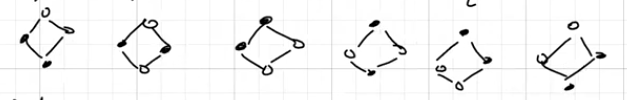
\includegraphics[scale=0.5]{skica_dokaza_posplositev_poly}
%		\caption{Vsa mo"zna barvanja z danimi parametri}
%	\end{figure}
%	To "se ni na"s rezultat, ker moramo izlo"citi ekvivalentna barvanja.
%	Pre"stejmo negibne to"cke. Pri identiteri jih je $6$ (vse), pri rotaciji za $180^{\circ}$ pa $2$.
%	Na desni strani Burnsidove leme dobimo
%	\[  \]
%\end{proof}

\section{Trije klasi"cni izreki iz teorije delno urejenih mno"zic}
\begin{defn}[Delno urejena mno"zica]
	Mno"zica opremljena z relacijo delne urejenosti $(P, \leqslant)$.
\end{defn}
\begin{rem}
	Izraz ``delno urejena mno"zica'' bomo kraj"sali z ``DUM'', ampak izgovorimo s celim izrazom. V angle"s"cini delno urejenim mno"zicam pravimo ``partially ordered sets'', kraj"samo ``poset'' in okraj"sano tudi izgovarjamo.
\end{rem}
\begin{defn}[Relacija delne urejenosti]
	Relacija, za katero veljajo naslednje lastnosti
	\begin{itemize}
		\item refleksivnost $x \leqslant x$
		\item antisimetri"cnost $x \leqslant y \land y \leqslant x \implies x = y$
		\item tranzitivnost $x \leqslant y \land y \leqslant z \implies x \leqslant z$
	\end{itemize}
\end{defn}
\begin{ex}
	Ozna"cujemo $\underline{n} \coloneqq ([n], \leqslant)$, kjer je $\leqslant$ obi"cajna relacija manj"se ali enako.
\end{ex}
\begin{ex}
	Boolova algebra $B_n \coloneqq (2^{[n]}, \subseteq)$. To je algebra za operaciji $\cup$, $\cap$. V ra"cunalni"stvu pogosto sre"camo dvoelementno Boolovo algebro $B_1 = \{0, 1\}$.
\end{ex}
\begin{ex}
	$D_n \coloneqq (\{\text{delitelji }n\}, |)$. Za mno"zico bi lahko vzeli tudi $\N_{>0}$
\end{ex}

\begin{defn}[Stroga neenakost]
	\[ x < y \iff x \leqslant y \land x \neq y\]
\end{defn}
\begin{defn}[Predhodnik]
	$x$ je predhodnik $y$, "ce sta v relaciji $\lessdot$
	\[ x \lessdot y \iff x < y \land \nexists z: x < z < y\]
\end{defn}
\begin{ex}
	$B_3 = \{\emptyset, \{1\}, \{2\}, \{3\}, \{1,2\}, \{1,3\}, \{2,3\}, \{1,2,3\}\}$. $A \in B_3$ je predhodnik elementov $A \cup \{i\}$ za vsak $i \notin A$.
\end{ex}

\begin{defn}[Hassejev diagram]
	Graf $(V, E)$, kjer so vozli"s"ca $V=P$ (elementi na"se mno"zice), robovi pa $E=\{(x,y); x \lessdot y \lor y \lessdot x\}$. Obi"cajno nari"semo tako, da je $y$ nad $x$, "ce je $x < y$.
\end{defn}
\begin{figure}[h!]
	\centering
	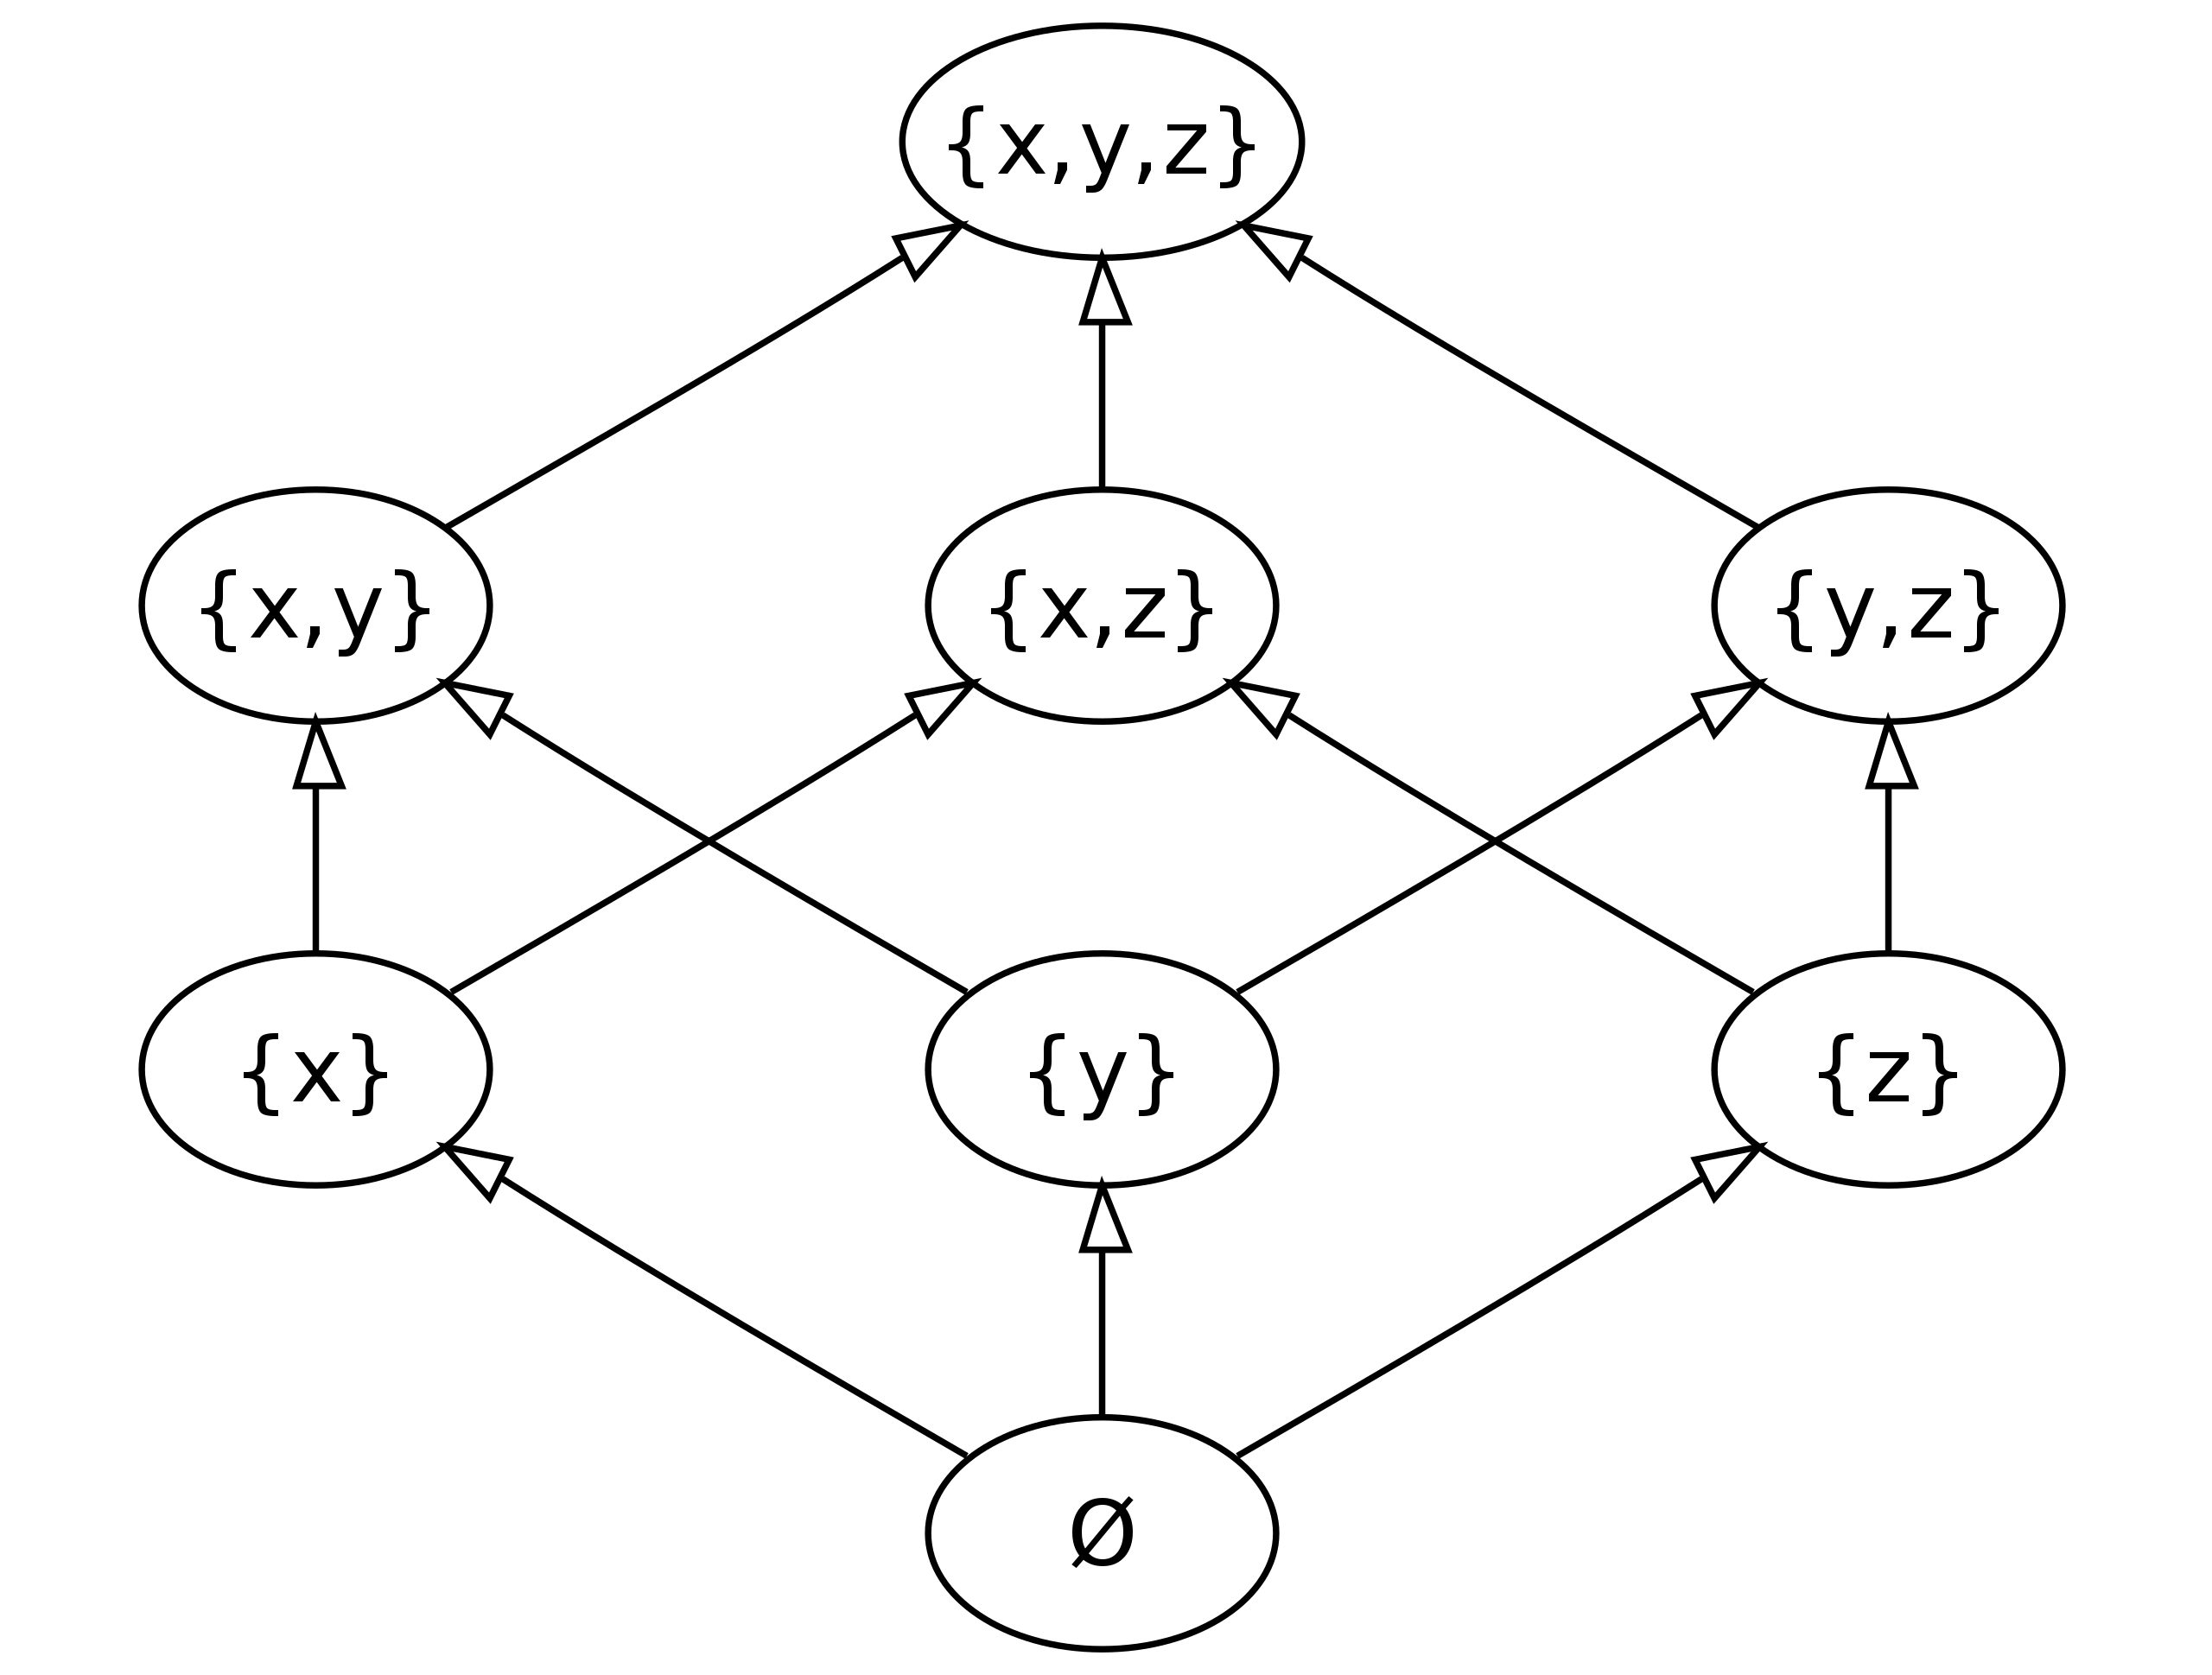
\includegraphics[scale=0.1]{hasse_b3}
	\caption{Hassejev diagram $B_3$}
\end{figure}
\begin{figure}[h!]
	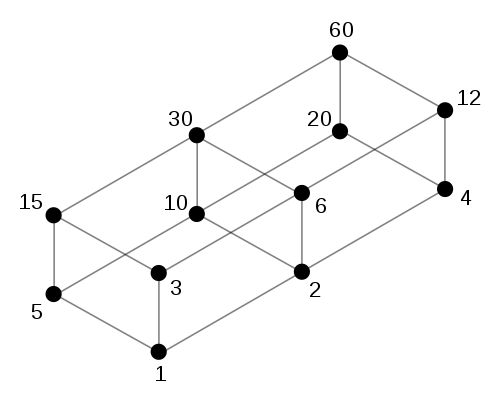
\includegraphics[scale=0.4]{hasse_d60}
	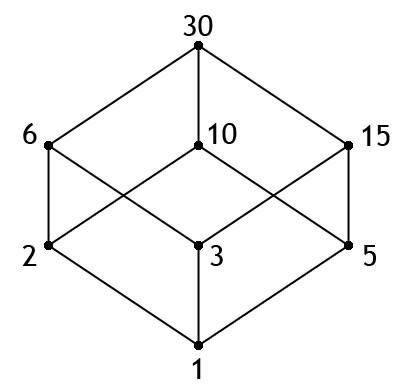
\includegraphics[scale=0.6]{hasse_d30}
	\caption{Hassejeva diagrama za $D_{30}$ in $D_{60}$}
\end{figure}
\begin{claim}
	Hassejev diagram $B_n$ je hiperkocka $Q_n$.
\end{claim}
\begin{claim}\label{Dn_je_hiperkocka}
	"Ce je $n$ produkt razli"cnih pra"stevil, je Hassejev diagram $D_n$ hiperkocka.
\end{claim}

\begin{defn}[Izomorfnost]
	Delno urejeni mno"zici $P$ in $Q$ sta izomorfni, "ce obstaja bijekcija $\phi: P \rightarrow Q$, da velja $a \leqslant b \iff \phi(a) \leqslant \phi(b)$.
\end{defn}
\begin{defn}[Kartezi"cni produkt]
	$P \times Q$ je delno urejena mno"zica z elementi $(x, y)$, $x \in P, y \in Q$, in relacijo $(x, y) \leqslant (x', y') \iff x \leqslant x' \land y \leqslant y'$.
\end{defn}
\begin{proof}
	Bralec lahko za zabavo doka"ze, da je kartezi"cni produkt delno urejenih mno"zic tudi delno urejena mno"zica.
\end{proof}

\begin{ex}
	$\underline{2} \times \underline{2} \times \cdots \times \underline{2} \cong B_n$. Izomorfizem doka"zemo z $\phi(A) \coloneqq (\varepsilon_1, \ldots, \varepsilon_n)$.
\end{ex}
\begin{ex}
	$n = p_1^{\alpha_1}p_2^{\alpha_2}\cdots p_k^{\alpha_k}$. Opazimo, da je $D_n$ izomorfen
	$[0, \alpha_1] \times [0, \alpha_2] \cdots \times [0,\alpha_k]$, kjer smo z $[0, \alpha_i]$ ozna"cili $\underline{\alpha_i} \cup \{0\}$.
\end{ex}
Iz zgornjih dveh primerov je razvidno, da "ce je $n$ produkt razli"cnih pra"stevil, je $D_n$ izomorfen $B_k$, kjer je $k$ mo"c faktorizacije $n$. Iz tega sledi zgornja trditev o Hassejevih diagramih $D_n$ (\ref{Dn_je_hiperkocka}).

\begin{defn}[Veriga]
	Naj bo $(P, \leqslant)$ delno urejena mno"zica. Tedaj je $(C \subseteq P, \leqslant)$ veriga, "ce velja $\forall x,y\in C: x \leq y \lor y \leq x$ (vsi elementi so med seboj primerljivi).
\end{defn}
\begin{ex}
	$\{ \emptyset, \{1, 3\}, \{1, 3, 4\}\} \subseteq B_4$ je veriga.
\end{ex}
\begin{defn}[Antiveriga]
	Naj bo $(P, \leqslant)$ delno urejena mno"zica. Tedaj je $(C \subseteq P, \leqslant)$ antiveriga, "ce velja $\forall x,y\in C: \lnot(x \leq y \lor y \leq x)$ (nobena dva elementa nista primerljiva).
\end{defn}
\begin{ex}
	$\{\{1, 3\}, \{2, 4\}, \{1, 2, 3\}\} \subseteq B_5$ je antiveriga.
\end{ex}

\begin{defn}[Vi"sina delno urejene mno"zice]
	Velikost najdalj"se verige.
\end{defn}
\begin{defn}["Sirina delno urejene mno"zice]
	Velikost najdalj"se antiverige.
\end{defn}
\begin{ex}
	\begin{tabular}{ccc}
		mno"zica & vi"sina & "sirina \\
		$\underline{n}$ & $n$ & $1$ \\
		$B_n$ & $n+1$ & $\binom{n}{\left\lfloor \frac{n}{2} \right\rfloor}*$ \\
		$D_n$ & $\alpha_1 + \cdots + \alpha_k + 1$ & ?\\
	\end{tabular}
\end{ex}
\begin{rem}
	* To je malo te"zje dokazati, ampak bomo pokazali kasneje (Spernerjev izrek).
\end{rem}
\begin{defn}[Maksimalni element]
	Tak $x$, da velja $\nexists y: x \leqslant y$.
\end{defn}
\begin{defn}[Najve"cji element]
	Tak $x$, da velja $\forall y: x \geqslant y$.
\end{defn}
\begin{rem}
	"Ce je $x$ najve"cji, potem je $x$ maksimalen. Obratno ne velja.
\end{rem}
\begin{rem}
	"Ce je $P$ kon"cna, obstaja maksimalen element.
\end{rem}
\begin{rem}
	Obstaja najve"c en najve"cji element.
\end{rem}

\begin{theorem}[Minskyjev izrek]
	Naj bo $(P, \leqslant)$ kon"cna delno urejena mno"zica, $M$ dol"zina najdalj"se verige (vi"sina), $m$ pa najmanj"se "stevilo antiverig, s katerimi lahko pokrijemo $P$. Tedaj velja $M = m$.
\end{theorem}
\begin{proof}
	O"citno velja $M \leqslant m$, saj bo vsak element najdalj"se verige moral imeti svojo antiverigo. $m \leqslant M$ bomo pokazali z indukcijo po mo"ci $P$.\\
	Baza indukcije: $|P| = 1$. $m = M = 1$.\\
	Indukcijski korak: definirajmo $A \coloneqq \{\text{maksimalni elementi v }P\}$. Vemo, da je vi"sina $P \setminus A$ je zagotovo $M-1$ (vsaka najdalj"sa veriga ima natanko en maksimalen element). Po indukcijski predpostavki jo zato lahko pokrijemo z $M-1$ antiverigami. Ker je $A$ antiveriga, lahko $P$ pokrijemo z $M$ antiverigami.
\end{proof}
\begin{rem}
	Ta dokaz slu"zi tudi kot algoritem za iskanje antiverig.
\end{rem}

\subsection{Dilworthov izrek}
\begin{theorem}[Dilworthov izrek]
	Naj bo $(P, \leqslant)$ kon"cna delno urejena mno"zica, $M$ dol"zina najdalj"se antiverige ("sirina), $m$ pa najmanj"se "stevilo verig, s katerimi lahko pokrijemo $P$. Tedaj velja $M = m$.
\end{theorem}
\begin{proof}
	Podobno kot pri Minskyjevem izreku, opazimo da $M \leqslant m$, ker mora vsak element najdalj"se antiverige imeti svojo verigo v pokritju. $m \leqslant M$ bomo pokazali z indukcijo po mo"ci $P$.\\
	Baza indukcije: $|P| = 1$. $m = M = 1$.\\
	Indukcijski korak: definirajmo $C \coloneqq$ katerakoli najdalj"sa veriga v $P$. Problem nastane (za razliko od dokaza Minskyjevega), ker $P \setminus C$ nima nujno manj"se "sirine kot $P$.
	
	"Ce je se "sirina zmanj"sala, lahko (enako kot pri Minskyjevem) $P\setminus C$ pokrijemo z $\leqslant M-1$ verigami, torej lahko $P$ pokrijemo z $\leqslant M$ verigami.
	
	"Ce se "sirina ni zmanj"sala, izberimo neko antiverigo $A=\{a_1, \ldots, a_n\}$ iz $P \setminus C$. Definirajmo
	\begin{itemize}
		\item $S^+ \coloneqq \{x \in P; \exists i: x \geqslant a_i\}$
		\item $S^- \coloneqq \{x \in P; \exists i: x \leqslant a_i\}$
	\end{itemize}
	Poka"zimo nekaj lastnosti glede $S^+$ in $S^-$.
	\begin{enumerate}
		\item $S^+ \cap S^- = A$
		\begin{proof}
			$A$ je o"citno vsebovan v obeh mno"zicah zaradi refleksivnosti ($\forall a \in A \exists i: a \leqslant a_i$). "Ce je $x \in S^+ \cap S^-$, potem $a_i \leqslant x \leqslant a_j$, zaradi tranzitivnosti pa $a_i \leqslant a_j$. Ker sta $a_i$ in $a_j$ iz iste antiverige, mora veljati $i=j$, kar pomeni da je $x = a_i$ in zato $x \in A$.
		\end{proof}
		\item $S^+ \cup S^- = P$
		\begin{proof}
			O"citno je, da je unija vsebovana v $P$. "Ce $x \notin S^+$ in $x \notin S^-$, potem $\forall i: x \not\geqslant a_i \land x \not\leqslant a_i$, kar pomeni da je $A \cup \{x\}$ antiveriga, ki je ve"cja od $A$, kar je v nasprotju z definicijo $A$.
		\end{proof}
		\item $S^+ \neq P$
		\begin{proof}
			Najmanj"si element v $C$ zagotovo ni v $S^+$; "ce bi obstajal $i$, da $x \geqslant a_i$, bi $C \cup \{a_i\}$ bila dalj"sa veriga kot $C$. Pomembno je opaziti, da $x \neq a_i$, ker je $A$ sestavljena iz elementov $P \setminus C$.
		\end{proof}
		\item $S^- \neq P$
		\begin{proof}
			Iz istega razloga kot zgoraj najve"cji element $C$ zagotovo ni v $S^-$.
		\end{proof}
	\end{enumerate}
	Z drugimi besedami, $S^+$ ima "sirino $M$, a je njena mo"c strogo manj"sa od $|P|$. Po indukcijski predpostavki lahko $S^+$ pokrijemo z $M$ verigami $C_1^+, \ldots, C_M^+$, $S^-$ pa z $C_1^-, \ldots, C_M^-$. Vsak element $A$ mora imeti svojo verigo $C_i^+$. Brez "skode za splo"snost privzemimo $a_i \in C_i^+$ in $a_i \in C_i^-$. Na"se pokritje $P$ja sestavljajo $C_i = C_i^+ \cup C_i^-$.
\end{proof}

\subsection{Spernerjev izrek}
\begin{lemma}
	$\forall k: \binom{n}{k} \leqslant \binom{n}{\left\lfloor \frac{n}{2} \right\rfloor}$. 
	Povedano z besedami: trdimo, da je najve"cji binomski koeficient neke vrstice vedno v njeni sredini.
\end{lemma}
\begin{proof}
	Oglejmo si zaporedna binomska koeficienta in izra"cunajmo kriterij, kdaj je naslednji ve"cji od prej"snjega.
	\[ \binom{n}{k} \leqslant \binom{n}{k+1} \]
	\[ \frac{\binom{n}{k}}{\binom{n}{k+1}}\leqslant 1 \]
	\[ \frac{n!(k+1)!(n-k-1)!}{k!(n-k)!n!} \leqslant 1 \]
	\[ \frac{k+1}{n-k} \leq 1 \]
	\[ k+1 \leq n-k \]
	\[ 2k+1 \leq n \]
	\[ k \leqslant \frac{n-1}{2} \]
\end{proof}
\begin{rem}
	% fun fact time
	Zaporedje, za katerega velja $a_0 \leqslant a_1 \leqslant \cdots \leqslant a_k \geqslant a_{k+1} \geqslant \cdots$ imenujemo unimodalno.
\end{rem}

\begin{theorem}[Spernerjev]
	"Sirina $B_n$ je $\binom{n}{\left\lfloor \frac{n}{2} \right\rfloor}$.
\end{theorem}
\begin{proof}
	"Ce vzamemo $A=\binom{\lbrack n \rbrack}{\left\lfloor \frac{n}{2} \right\rfloor}$ je to ravno antiveriga velikosti $\binom{n}{\left\lfloor \frac{n}{2} \right\rfloor}$. S tem smo fiksirali minimalno vrednost "sirine. Doka"zimo, da ne obstaja dalj"sa antiveriga.
	
	Naj bo $A$ poljubna antiveriga v $B_n$. Naj bo $a_i$ "stevilo elementov $A$, ki so $i$-elementne mno"zice. O"citno je $a_0 + a_1 + \cdots + a_n = |A|$.
	
	Pre"stejmo maksimalne verige v $B_n$
	\begin{itemize}
		\item Vse: $n!$
		\begin{proof}
			Verigo $\emptyset \subseteq \{i_1\} \subseteq \{i_1, i_2\} \subseteq \cdots \subseteq [n]$ dobimo tako, da izberemo nek vrstni red dodajanja elementov proti $[n]$.
		\end{proof}
		\item Tiste, ki vsebujejo izbrano podmno"zico $S \subseteq B_n$ velikosti $k$: $k!(n-k)!$
		\begin{proof}
			Dobimo jih tako, da konstruiramo verigo do $S$ ($k!$ na"cinov), nato pa dodajamo "se ostalih $n-k$ elementov do $[n]$.
		\end{proof}
		\item Tiste, ki vsebujejo katerikoli element iz $A$: $\sum_{k=0}^na_kk!(n-k)!$
		\begin{proof}
			Vsak element $A$ ima lahko med $0$ in $n$ elementov. "Ce za vsako od teh "stevil dodamo se"stejemo "stevilo verig, ki vsebuje ta element (teh je dokazano $k!(n-k)!$), dobimo ravno na"s rezultat. Nobene verige nismo "steli dvakrat, ker vsaka od na"sih verig vsebuje natanko en - unikaten - element $A$-ja.
		\end{proof}
	\end{itemize}
	Zaklju"cimo lahko, da je $\sum_{k=0}^na_kk!(n-k)! \leq n!$, saj je mno"zica maksimalnih verig, ki vsebujejo elemente iz $A$ pomno"zica vseh maksimalnih verig. "Ce delimo z $n!$, dobimo
	\[\sum_{k = 0}^n\frac{a_k}{\binom{n}{k}} \leq 1\]
	\[
		1 \geq
		\sum_{k = 0}^n\frac{a_k}{\binom{n}{k}} \geq
		\sum_{k = 0}^n\frac{a_k}{\binom{n}{\left\lfloor\frac{n}{2}\right\rfloor}} =
		\frac{1}{\binom{n}{\left\lfloor\frac{n}{2}\right\rfloor}}\sum_{k = 0}^na_k
	\]
	\[\binom{n}{\left\lfloor\frac{n}{2}\right\rfloor} \geq \sum_{k=0}^na_k\]
	\[\binom{n}{\left\lfloor\frac{n}{2}\right\rfloor} \geq |A|\]
\end{proof}

\begin{conseq}[Dilworth-Sperner]
	$B_n$ lahko pokrijemo z $\binom{n}{\left\lfloor\frac{n}{2}\right\rfloor}$ verigami.
\end{conseq}

\subsection{Hallov izrek}
\begin{defn}[Prirejanje]
	Naj bo $G=(V, E)$ graf. $M \subseteq E$ je prirejanje, "ce velja $e \cap f = \emptyset$ za vsaka $e, f \in M$.
\end{defn}
"Ce pobarvamo povezave iz $M$ z rde"co barvo, potem nobeno vozli"s"ce iz $G$ nima ve"c kot ene rde"ce povezave.
\begin{defn}[Popolno prirejanje]
	Naj bo $M$ prirejanje grafa $G$. $M$ je popolno prirejanje, "ce velja $\forall v \in V: \exists e \in M: v \in e$.
\end{defn}
\begin{rem}
	Angle"sko: ``matching'' in ``perfect matching''.
\end{rem}
\begin{rem}
	"Ce ima $G$ popolno prirejanje, je $|V|$ sodo.
\end{rem}
\begin{defn}[Popolno prirejanje iz $X$ v $Y$]
	Naj bo $G$ dvodelen graf na particiji $X$ in $Y$. Prirejanje $M$ je popolno prirejanje iz $X$ v $Y$ "ce velja $\forall x \in X: \exists e \in M: x \in e$.
\end{defn}
\begin{rem}
	"Ce obstaja popolno prirejanje iz $X$ v $Y$, je $|X| \leq |Y|$. Popolno prirejanje namre"c deluje kot injekcija.
\end{rem}
\begin{defn}[Sose"s"cina $A$]
	$N(A) = \{v \in V: \exists u \in A: u \sim v\}$
\end{defn}
\begin{rem}
	"Ce obstaja popolno prirejanje iz $X$ v $Y$, je $|A| \leq |N(A)|$. Popolno prirejanje je v tem primeru injekcija $A \rightarrow N(A)$.
\end{rem}
\begin{defn}[Alternirajo"ca pot]
	Pot, v kateri se izmenjujejo rde"ce in "crne povezave (tj. povezave, ki so element prirejanja in povezave, ki niso).
\end{defn}
\begin{theorem}[Hall]
	Naj bo $G$ dvodelen graf na particiji $X$ in $Y$. Tedaj obstaja popolno prirejanje iz $X$ v $Y$ natanko tedaj, ko $|A| \leqslant |N(A)|$ za vsak $A \subseteq X$.
\end{theorem}
\begin{rem}
	"Ce predpostavimo Dilworthov izrek, je Hallov izrek zelo lahko dokazati. Velja tudi obratno.
\end{rem}
\begin{rem}
	Hallov izrek nam poda ekvivalenco oblike $\exists \iff \forall$. Tako ekvivalenco imenujemo dobra karakterizacija. Kadar imamo tako ekvivalenco, lahko doka"zemo ali ovr"zemo trditev na levi ali desni strani s tem da doka"zemo obstoj najve"c enega objekta.
	
	% A to rabimo?
	% "Se en primer dobre karakterizacije je izrek o Eulerjevih grafih, ki trdi, da je povezan graf Eulerjev (obstaja Eulerjev obhod) natanko tedaj, ko so vsa vozli"s"ca sode stopnje.
	% Za obstoj Hamiltonovega cikla nimamo dobre karakterizacije.
\end{rem}
\begin{proof}
	Dokaz v desno smo "ze razmislili. Za"cnimo s poljubnim prirejanjem in predpostavimo $|A| \leqslant |N(A)|$. "Ce je to prirejanje popolno iz $X$ v $Y$, potem smo kon"cali. Sicer poskusimo to prirejanje pove"cati. To bomo lahko ponavljali, dokler ne pridemo do popolnega prirejanja.
	
	Po predpostavi (na"se prirejanje ni popolno) obstaja neko vozli"s"ce $a \in X$, ki ni v nobeni povezavi v prirejanju (ni element rde"ce povezave). Definirajmo \\
	$A \coloneqq \{x \in X; \exists \text{ alternirajo"ca pot od }a\text{ do }x\}$ in\\
	$B \coloneqq \{y \in Y; \exists \text{ alternirajo"ca pot od }a\text{ do }y\}$.
	
	Zagotovo velja $a \in A$. Poka"zimo, da je $N(A) \subseteq B$.
	\[y \in N(A) \implies \exists x \in A: x \sim y \implies \exists \text{ alternirajo"ca pot od }a\text{ do }x, x \sim y\]
	Ker smo v dvodelnem grafu in ker $a$ nima rde"cih povezav, bo zadnja povezava v alternirajo"ci poti do $x$ rde"ca (v $Y$ vedno pridemo po "crni in v $X$ vedno pridemo po rde"ci). "Ce je povezava $xy$ "crna, potem jo lahko dodamo k alternirajo"ci poti in dobimo alternirajo"co pot od $a$ do $y$, torej je $y \in B$. "Ce pa je $xy$ rde"ca, mora biti $y$ predzadnje vozli"s"ce na"se poti od $a$ do $x$, ker ima $x$ lahko najve"c eno rde"co povezavo (tisto, po kateri smo pri"sli do njega). Torej je $y \in B$.
	
	Po predpostavki in pravkar"snji ugotovitvi, imamo
	\[ |A| \leqslant |N(A)| \leqslant |B| \]
	Iz $A$ gre $|A|-1$ rde"cih povezav (vsi elementi razen $a$ morajo imeti natanko eno rde"co povezavo, ker so del alternirajo"ce poti). To pomeni, da v $B$ obstaja vozli"s"ce $b$, ki nima nobene rde"ce povezave (ker je $|A|\leqslant|B|$). "Ce vsem povezavam v poti od $a$ do $b$ zamenjamo barvo, ne bomo pokvarili prirejanja; vsako vozli"s"ce bo imelo "se vedno najve"c eno rde"co povezavo. Ker se alternirajo"ca pot od $a$ do $b$ za"cne in kon"ca s "crno, smo s to inverzijo hkrati pove"cali "stevilo rde"cih povezav za $1$.
	
	Postopek ponavljamo dokler ne dose"zemo popolnega prirejanja.
\end{proof}
\begin{rem}
	To je algoritem, ki bodisi poi"s"ce popolno prirejanje, bodisi doka"ze, da le-to ne more obstajati ("ce slu"cajno naletimo na primer, ko $|A| > |N(A)|$).
\end{rem}

\begin{conseq}
	Naj bo $G$ dvodelni graf na $X$ in $Y$. Tedaj velja
	\[ \forall x \in X: \forall y \in Y: \deg(x) \geqslant \deg(y) \implies \exists \text{ popolno prirejanje } X\rightarrow Y \]
\end{conseq}
\begin{proof}
	"Zelimo pokazati, da je $|A| \leqslant |N(A)|$. Ozna"cimo "stevilo povezav med $A$ in $B$ kot $e(A, B)$ in $B \coloneqq N(A)$. Naj bo $d$ neko "stevilo, ki je med $\deg(x)$ in $\deg(y)$ za vsaka $x$ in $y$ ($d$ obstaja po na"si predpostavki).
	
	\[d \cdot |B| \geqslant \sum_{y \in B}\deg(y) \geqslant e(A,B) = \sum_{x\in A}\deg(x) \geqslant d\cdot |A|\]
	\[\implies |A| \leqslant |B|\]
	Po Hallovem izreku je to vse, kar moramo pokazati.
\end{proof}

\begin{conseq}
	Naj bo $G$ biregularen (stopnja vsakega vozli"s"ca na levi/desni strani je enaka) dvodelen graf. Tedaj obstaja popolno prirejanje iz $X$ v $Y$ ali iz $Y$ v $X$.
\end{conseq}
\begin{proof}
	\[ |E| = \sum_{x \in X}\deg(x) = r\cdot |X| \]
	\[ |E| = \sum_{y \in Y}\deg(y) = s\cdot |Y| \]
	\[ |X| \leqslant |Y| \iff r \geqslant s \iff \exists \text{ popolno prirejanje }X\rightarrow Y \]
	\[ |X| \geqslant |Y| \iff r \leqslant s \iff \exists \text{ popolno prirejanje }Y\rightarrow X \]
\end{proof}

% tukej bi lahko dodal se kksn primer

\end{document}
